%!TEX root = ../main.tex

%%%%%%%%%%%%%%%%%%%%%%%%%%%%%%%
%%%%%%%%%%%%%%%%%%%%%%%%%%%%%%%
\chapter{Fundamentals}
% Evtl. lieber Basics nennen; Stand der Technik ist es ja nicht wirklich
\label{chap:fundamentals}

The sections \ref{sec:basics-sg}, \ref{sec:system-stability}, \ref{sec:numerical-methods} of the following chapter are recitations of various fundamental literature \autocite{oedingElektrischeKraftwerkeUnd2016,schwabElektroenergiesystemeSmarteStromversorgung2022,georgievNumericalAnalysisTime2022,milesNumericalMethodsPython2023,langtangenPrimerScientificProgramming2016,machowskiPowerSystemDynamics2020,kundurPowerSystemStability2022}. Paragraphs specifically from selected sources are marked as such. 

% General sources in terms of standard literature: \autocite{oedingElektrischeKraftwerkeUnd2016,gloverPowerSystemAnalysis2017,kundurPowerSystemStability2022,machowskiPowerSystemDynamics2020}

%%%%%%%%%%%%%%%%%%%%%%%%%%%%%%%
\section{Basics synchronous generators}
\label{sec:basics-sg}
% \commenting{
%         \begin{itemize}
%                 \item characteristics of a synchronous generator; structure and types of SG's
%                 \item mathematical background and description of the behavior -> dynamic modelling
%                 \item \textbf{Swing equations}
%                 \item Damping: not interesiting for us
%         \end{itemize}
% }

Synchronous generators (\acs{SG}) are used for electric power generation and thus connected to a mechanical power or toque input. For power plants most of the time this is a (steam) turbine. The main two types are the high-speed generator (often turbogenerator) and the low speed generator (see \autoref{fig:generators}). \autocite{machowskiPowerSystemDynamics2020,oedingElektrischeKraftwerkeUnd2016}

\begin{figure}[H]
        \centering
        \begin{subfigure}[b]{.49\textwidth}
                \centering
                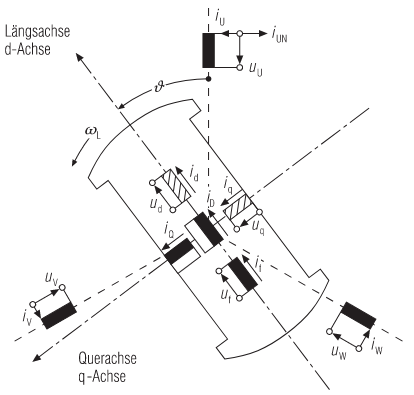
\includegraphics[width=.9\textwidth]{schenkelpol.png}
                \subcaption{low speed configuration}
        \end{subfigure}
        \begin{subfigure}[b]{.49\textwidth}
                \centering
                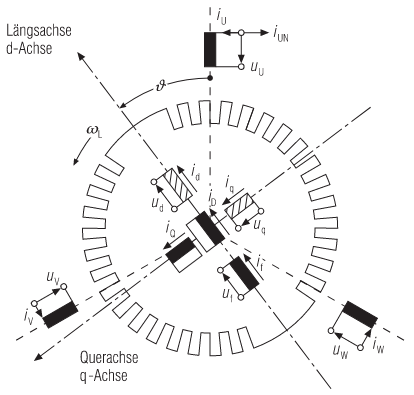
\includegraphics[width=.9\textwidth]{turbolaeufer.png}
                \subcaption{high speed configuration}
        \end{subfigure}
        \caption[Types of \acfp{SG}]{Schematic view of types of \acfp{SG}; from \autocite{oedingElektrischeKraftwerkeUnd2016}}
        \label{fig:generators}
\end{figure}

Generators have a static part, the stator, and the moving rotor. The magnetic windings in the rotor are excited with an excitation voltage, the rotor is then turning inside the stator with the power of the turbine. In the stator a three phase current is injected and can be used for delivering electrical power to a connected grid. The whole principle is a balance between the electromagnetic forces, if the demanded power connected to the stator is too high, the rotor will slow down and vice versa. Usually these generators have so called damper windings, which damp this dynamic behavior. For this research paper, the damping effect is neglected. As well the regulation of the excitation voltage is seen as too complex for this paper. Further information is given in the sources \autocite{machowskiPowerSystemDynamics2020,kundurPowerSystemStability2022,oedingElektrischeKraftwerkeUnd2016,schwabElektroenergiesystemeSmarteStromversorgung2022}. Relevant for this paper is the so called swing equation, which is describing the dynamic behavior of the \acs{SG}.

The final swing equation system can be derived to following two equations, which have to be solved in every time step to determine the pole angle $\delta$ and the rotor speed $\omega$, respectively the rotor speed change from its base value $\Delta\omega$:
\begin{align}
        \frac{d\delta}{dt}       & =\Delta\omega \label{eq:swing1}                                                         \\[12pt]
        \frac{d\Delta\omega}{dt} & =\frac{1}{2 \cdot H_\mathrm{gen}} \cdot (P_\mathrm{m} - P_\mathrm{e}) \label{eq:swing2}
\end{align}
where

\begin{tabularx}{\textwidth}[H]{ll}
        $\delta$                & power angle \\
        $\Delta\omega$          & change of rotor angular speed \\
        $H_\mathrm{gen}$        & inertia constant of the \acs{SG} \\
        $P_\mathrm{m}$          & mechanical power of the turbine \\
        $P_\mathrm{e}$          & electrical power demanded transferred out of the \acs{SG}
\end{tabularx}
\vspace{12pt}

% The generation of a \ac{TDS} for this equation system takes place in \autoref{sec:tds}.

%%%%%%%%%%%%%%%%%%%%%%%%%%%%%%%
\section{System stability esp. transient context}
\label{sec:system-stability}
\commenting{
        \begin{itemize}
                \item What is to be analyzed? And why? -> different stability analysis
                \item rotor angle stability,
                \item \textbf{derivation of EAC,}
                \item basic assessment models (single machine infinite bus, see \autocite{kundurPowerSystemStability2022})
        \end{itemize}
}

With respect to the limitations, that
\begin{enumerate}
        \item the machine is operating under balanced three-phase positive-sequence conditions,
        \item the machine excitation is constant,
        \item the machine losses, saturation, and saliency are neglected,
\end{enumerate}
a simplified \acf{SMIB} model can be considered for transient stability assessment (see \autoref{fig:smib-model}).  The \ac{IBB} is working with a constant voltage $E_\mathrm{ibb}$ and angle $\delta_\mathrm{ibb}$, typically set to $0^\circ$. The real power flowing from the \ac{SG} to the \ac{IBB} is then expressed within the \autoref{eq:p_e} and only dependent on the power angle $\delta$. The reactance $X_\mathrm{res}$ is expressing the simplified reactance from the respective circuit.
\begin{align}
        P_\mathrm{e}=\frac{E_\mathrm{p} \cdot E_\mathrm{ibb}}{X_\mathrm{res}} \cdot sin(\delta) \label{eq:p_e}
\end{align}
The mechanical power of the turbine is assumed constant, due to the short occurance of transient stability problems.

\begin{figure}[H]
        \centering
        \vspace{1cm}
        \begin{circuitikz}[european, scale=.9, smallR/.style={resistor,resistors/scale=.7}]
                \draw (0,0) node[oscillator, anchor=east, name=gen]{} --(.5,0)
                to[L, name=X_g] ++(2,0) coordinate(f1)
                % \bushere{1}{$\underline{E}_\mathrm{T}'$}{}
                % to[oosourcetrans,prim=delta,sec=wye] ++(2,0)
                \bushere{2}{$\underline{V}_\mathrm{bb}$}{\acs{SG} bus bar} coordinate(b1) ++(0,-1) -- ++(.25,0) -- coordinate(f2) ++(1.75,0)
                to[L, name=X_l3] ++(1,0) -- ++(1.5,0) ++(0,1)
                \bushere{2}{$E_\mathrm{ibb}~\angle~0^{\circ}$}{\acs{IBB}} ++(0,1) coordinate(b2) ++(0,-1) coordinate(b3) -- ++(.75,0) coordinate(f3) -- ++(.75,0) to[L, name=X_ibb] ++(1,0) -- ++(1,0)
                node[gridnode, anchor=left, name=ib]{};

                % draw other resistances
                \draw (b1) ++(0,1) -- ++(.5,0) to[L, name=X_l1] (b2);
                \draw (b1) -- ++(.5,0) to[L, name=X_l2] (b3);
                % \draw[line width=2pt] (2.25,1) -- (2.25,-1);
                % \draw[line width=2pt] (4.75,1) -- (4.75,-1);
                % \draw[line width=2pt] (8.25,1) -- (8.25,-1);

                % labels for the resistors
                \node[above=6pt] at (X_g) {$X_\mathrm{g}'$};
                \node[above=6pt] at (X_ibb) {$X_\mathrm{ibb}$};
                \node[above=6pt] at (X_l1) {$3~X_\mathrm{l}$};
                % \node[below=6pt] at (X_l2) {$X_\mathrm{l}$};
                % \node[below=6pt] at (X_l3) {$X_\mathrm{l}$};

                % pole voltages and angles
                \path[->] (-1.2,.5) edge [bend right] node[left=6pt]{$E_\mathrm{p}~\angle~\delta$} (-1.2,-.5);
                % \path[->] (ib) ++(.8,.5) edge [bend left] node[right=6pt]{$E_\mathrm{ibb}~\angle~0^{\circ}$} ++(0,-1);

                % faults
                % \draw[-Stealth, very thick, red] (f1) ++(0,-.5) -- ++(-.15,-.45) -- ++(.3,.2) -- ++(-.2,-.6) coordinate(f1_text);
                % \node[below, red] at (f1_text) {\scriptsize fault 1};
                \draw[-Stealth, very thick, red] (f2) ++(0,.3) -- ++(-.15,-.45) -- ++(.3,.2) -- ++(-.2,-.6) coordinate(f2_text);
                \node[below, red, align=center] at (f2_text) {\scriptsize fault 2/3};
                \draw[-Stealth, very thick, red] (f3) ++(0,.3) -- ++(-.15,-.45) -- ++(.3,.2) -- ++(-.2,-.6) coordinate(f3_text);
                \node[below, red] at (f3_text) {\scriptsize fault 1};
        \end{circuitikz}
        \vspace{.5cm}
        \caption[Representative circuit of a \acf{SMIB} model]{Representative circuit of a \acf{SMIB} model with pole wheel voltage $E_\mathrm{p}~\angle~\delta$ and \acf{IBB} voltage $E_\mathrm{ibb}~\angle~0^{\circ}$; positions of considered faults 1 to 3 are marked with red lightning arrows}
        \label{fig:smib-model}
\end{figure}
where

\begin{tabularx}{\textwidth}[H]{lX}
        $\delta$                        & power angle (difference) \\
        $E_\mathrm{p}$                  & pole voltage of the \acf{SG} \\
        % $\underline{E}_\mathrm{T}'$     & complex potential on the primary side of the transformer \\
        % $\underline{E}_\mathrm{T}''$    & complex potential on the secondary side of the transformer \\
        % $\underline{E}_\mathrm{ibb}$    & complex pole potential of the \acf{IBB} \\
        $X_\mathrm{g}'$                 & reactance of the \acf{SG} \\
        $X_\mathrm{l}$                  & reactance of a single line \\
        $X_\mathrm{ibb}$                  & reactance of the \acf{IBB} \\
\end{tabularx}

\newpage
\section{Analytical calculation of the critical clearing time}
\label{sec:analytical-method}

\begin{wrapfigure}{r}{.6\textwidth}
        \centering
        % \missingfigure[figwidth=.4\textwidth]{Equal are criterion visualization}
        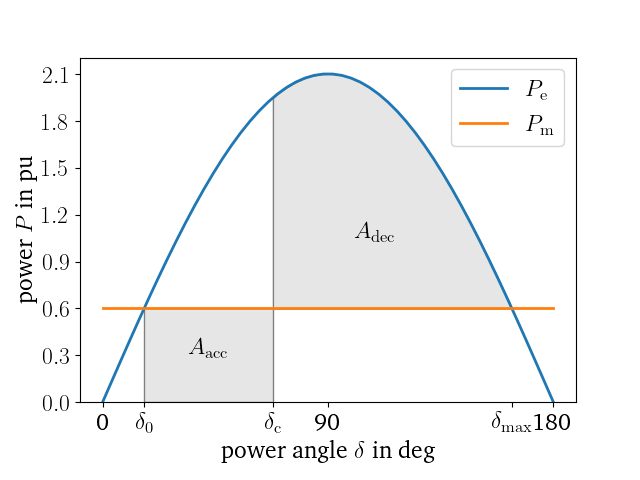
\includegraphics[width=.6\textwidth]{python/plots/eac.png}
        \caption{Illustrated \acf{EAC} in the P-$\delta$-curve where $A_\mathrm{acc}=A_\mathrm{dec}$}
        \label{fig:eac}
\end{wrapfigure}
For the analytical solution of the swing equation and following the \acs{CCT}, there is the need to find the critical power angle $\delta_\mathrm{cc}$ first. For this, the most common approach is the \acf{EAC}, considering that the amount of stored energy through acceleration (during the short or failure) is equal to the released energy (decelerating the rotor) when synchronizing again. These both energys can be calculated through the area under the curve of the power difference $\Delta P=P_\mathrm{m}-P_\mathrm{e}$, while the accelerating area is between the first stable operating angle $\delta_\mathrm{0}$ and the clearing angle $\delta_\mathrm{c}$, the decelerating area between $\delta_\mathrm{c}$ and the maximum dynamically stable angle $\delta_\mathrm{max}$. \autoref{fig:eac} is illustrating this approach. Following this approach a generalized expression is formed to
\begin{align}
        \int_{\delta_\mathrm{0}}^{\delta_\mathrm{1}}\Delta P~d\delta = 0 \label{eq:gen-eac},
\end{align}
while the more expressive can be achieved through splitting up the integral borders and equalize both areas:
\begin{align}
        % A_\mathrm{acc}=A_\mathrm{dec} \nonumber \\
        \int_{\delta_\mathrm{0}}^{\delta_\mathrm{c}}(P_\mathrm{m}-P_\mathrm{e})~d\delta = \int_{\delta_\mathrm{c}}^{\delta_\mathrm{max}}(P_\mathrm{e}-P_\mathrm{m})~d\delta \label{eq:big-eac}
\end{align}
With consideration of $\delta_\mathrm{max}=\pi-\delta_\mathrm{0}$, $P_\mathrm{e,normal}=P_\mathrm{max} \cdot sin(\delta_\mathrm{0})$, $P_\mathrm{e,fault}=0$, and some rearrangements, this leads to the final expression of the critical clearing angle:
\begin{align}
        \delta_\mathrm{cc}=arccos\big[~sin(\delta_\mathrm{0}) \cdot (\pi-2 \cdot \delta_\mathrm{0})-cos(\delta_\mathrm{0})~\big] \label{eq:delta-cc}
\end{align}

The second step is the calculation of the \acs{CCT} dependent on the critical clearing angle. Splitting the differentiated variables $d^2\delta$ and $dt$ in the combined swing equation and integrating twice, leads to the equation
\begin{align}
        \delta=\frac{\omega \cdot \Delta P}{4 H_\mathrm{gen}} \cdot t^2 + \delta_\mathrm{0}. \nonumber
\end{align}
Rearranging this gives an expression for calculating the critical clearing time $t_\mathrm{cc}$ (see \autoref{eq:tcc}).
\begin{align}
        t_\mathrm{cc}=\sqrt{\frac{4 H_\mathrm{gen} \cdot (\delta_\mathrm{cc}-\delta_\mathrm{0})}{\omega \cdot \Delta P}} \label{eq:tcc}
\end{align}
Both expressions \autoref{eq:delta-cc} and \autoref{eq:tcc} are only valid for clearing faults with an electric power drawing of $0~\mathrm{p.u.}$. For a partial line or power fault, the expressions tend to complicate more. One have to use $P_\mathrm{e}=P_\mathrm{max,~fault} \cdot sin(\delta)$ before both integrations of the area equations and the swing equation itself. Finally giving two expressions for the critical power angle $\delta_\mathrm{cc}$ and the \acs{CCT} $t_\mathrm{cc}$:
\mycomment[MK]{Sinnvoll da den vollständigen Rechenweg in den Anhang mit aufzunehmen?}
\begin{align}
        \delta_\mathrm{cc}=&~arccos\Bigg[\frac{P_\mathrm{m}}{P_\mathrm{max}-P_\mathrm{max,~fault}} \cdot (\pi-2 \cdot \delta_\mathrm{0})-\frac{P_\mathrm{max,~fault}}{P_\mathrm{max}-P_\mathrm{max,~fault}} \cdot cos(\delta_\mathrm{0}) \nonumber \\& - \frac{P_\mathrm{max}}{P_\mathrm{max}-P_\mathrm{max,~fault}} \cdot cos(\delta_\mathrm{0})~\Bigg] \label{eq:delta-cc-adv} \\[12pt]
        t_\mathrm{cc}=&\sqrt{\frac{4 H_\mathrm{gen} \cdot (\delta_\mathrm{cc}-\delta_\mathrm{0})}{\omega \cdot (P-P_\mathrm{max,~fault} \cdot sin(\delta_\mathrm{cc}))}} \label{eq:tcc-adv}
\end{align}\mycomment[MK]{Für den zweiten Fall erscheint mir die Berechnung der CCT etwas hoch -> P\_e auch nicht von t abhängig... Muss ich da einfach statt $\delta_cc$ die zeitabhängige $\delta$-Gleichung einsetzen?}

%%%%%%%%%%%%%%%%%%%%%%%%%%%%%%%
\section{Numerical methods for system modeling}
\label{sec:numerical-methods}

System dynamics is a method for describing, understand, and discuss complex problems in the context of system theory \textbf{[SOURCE]}. They often can be described through a set of coupled \acfp{ODE}, most resoluted in time dimension. \acsp{ODE} can be solved through numerical integration with different methods. An easy and less complex method is Euler's method. It uses a linear extrapolation to calculate the functions value at the next timestep, so following the iterable function
\begin{align}
        f_\mathrm{t+1}=f_\mathrm{t}+\left(\frac{df}{dt}\right)_\mathrm{t} \cdot \Delta t \label{eq:euler},
\end{align}
with $t$ being the time and $f$ an on $t$ dependent function. Generally a system of second order \acsp{ODE} can be rewritten as two first order equations. This often simplifies the calculation or the use of numerical methods. The presented swing equation of a \acs{SG} in \autoref{eq:swing1} and \autoref{eq:swing2} has been split up by that principle.

Python is providing a hanful of solvers, which can solve such first and second order \acsp{ODE}. As for this paper, the efficiency and run-time or error of the solver is not in the scope, simply the solver {\itshape odeint()} from the package {\itshape scipy} is used. The problem is thus explicitly solved. 

%%%%%%%%%%%%%%%%%%%%%%%%%%%%%%%
%%%%%%%%%%%%%%%%%%%%%%%%%%%%%%%
\chapter{Numerical modeling}
\label{chap:methods}

Following chapter will describe the implementation of Python Code for solving the derived \acs{ODE} system (see \autoref{sec:basics-sg}). For this the Python version 3.9 was used, in combination with the packages scipy, numpy, and matplotlib.\footnote{documentation and manual can be found on \href{https://scipy.org/}{\itshape https://scipy.org/} \autocite{virtanenSciPyFundamentalAlgorithms2020}, similiar for \href{https://matplotlib.org/}{\itshape matplotlib}, and \href{https://numpy.org/}{\itshape numpy} packages} % The complete code is included in the \autoref{app:code}.
% The complete Code of the main model with an example fault, as well as the parameter sets of the three considered faults is included in \autoref{app:code}.

%%%%%%%%%%%%%%%%%%%%%%%%%%%%%%%
\section{Structure of the \acs{CCT} assessment}

The central interest in the algorithm is to determine the time, until a system failure has to be resolved, so that it can remain stable and synchronized. In general, an enough accurate and easy approach for a \acf{SMIB} system is the \acf{EAC}. For a more complex and coupled machine system, other approaches are more targeting \autocite{batchuComparativeStudyEqual2022}. Further interest is to determine the associated crictical clearing angle. This is the maximum possible power angle at the \acs{CCT}, with which the fault can just be cleared into a stable system. At last one is interested in the time domain solution, just shortly before and after the \acs{CCT}. This shall illustrate the convergent and divergent behavior of the power angle and therefore the rotor speed.

\begin{figure}[h]
        \centering
        \begin{tikzpicture}[node distance = 1.5cm, auto]
                % Place nodes
                \node [papStart] (start) {start};
                \node [papProcess, below of = start, yshift= -2mm] (pro1){initialize start and simulation parameters};
                \node [papPredProc, below of = pro1, yshift= -5mm] (pro2){\nodepart{two} \shortstack{do \acs{TDS} with\\constant fault}};
                \node [papProcess, below of = pro2, yshift= -5mm] (pro3){determine \acs{CCT} and critical angle};
                \node [papPredProc, below of = pro3, yshift= -7mm](pro4){\nodepart{two}\shortstack{solving \acs{TDS}\\stable and unstable}};
                \node [papProcess, below of = pro4, yshift= -5mm](pro5){plot results};
                \node [papEnd, below of = pro5, yshift= -2mm] (end) {end};

                \node [right of = pro4, xshift=25mm] (iter) {\footnotesize\itshape{iterate 1x}};
                \node [right of = pro1, xshift=25mm] () {\footnotesize\itshape{init()}};
                \node [right of = pro2, xshift=25mm] () {\footnotesize\itshape{odeint()}};
                \node [right of = pro3, xshift=25mm] () {\footnotesize\itshape{determine\_cct()}};

                % Place joins
                \coordinate [above = of pro4, yshift= -9mm] (join1);
                \coordinate [below of = pro4, yshift= 5mm] (join2);

                % Draw edges
                \path [papLine] (start) -- (pro1);
                \path [papLine] (pro1) -- (pro2);
                \path [papLine] (pro2) -- (pro3);
                \path [papLine] (pro3) -- (pro4);
                \path [papLine] (pro4) -- (pro5);
                \path [papLine] (pro5) -- (end);
                \path [papLine] (join2) -| (iter);
                \path [papLine] (iter) |- (join1);
                % \path [papLine] (dec1) -- node [above] {\papNo} (predproc1);
                % \path [papLine] (predproc1) -- (pro3);
                % \path [papLine] (pro3) |- (join1);
        \end{tikzpicture}
        \caption[Program plan proposal for determining the \acf{CCT}]{Program plan proposal for determining the \acf{CCT} $t_\mathrm{cc}$, critical power angle $\delta_\mathrm{cc}$ and the \acf{TDS} of the \acf{SMIB}-model; including the associated main function name}
        \label{fig:program-plan}
\end{figure}

\autoref{fig:program-plan} illustrates the rough stucture of the numerical calculation. The single processes are further described in \autoref{sec:tds} for the time resoluted solving with {\itshape odeint()}, and \autoref{sec:eac} for the function {\itshape determine\_cct()}. 
% The initiialziation and plotting are documented via the complete code in \autoref{app:code}. 
The iterative solving of stable and unstable regie solutions is, neglecting the fault start and ending as initial conditions, an identical procedure and using the same function set as the described \acs{TDS}.

%%%%%%%%%%%%%%%%%%%%%%%%%%%%%%%
\section{Electrical simplifications and scenario setting}
\label{sec:scenario}

\subsection{Electric networks}
\label{sec:el-networks}

The \acs{SMIB}-model presented in \autoref{fig:smib-model} has to be devided into the two states {\itshape during fault} and {\itshape steady state}, and can further be simplified. This leads to a single replacement reactance and is more easy to use in the simulation.

\begin{figure}[H]
        \centering
        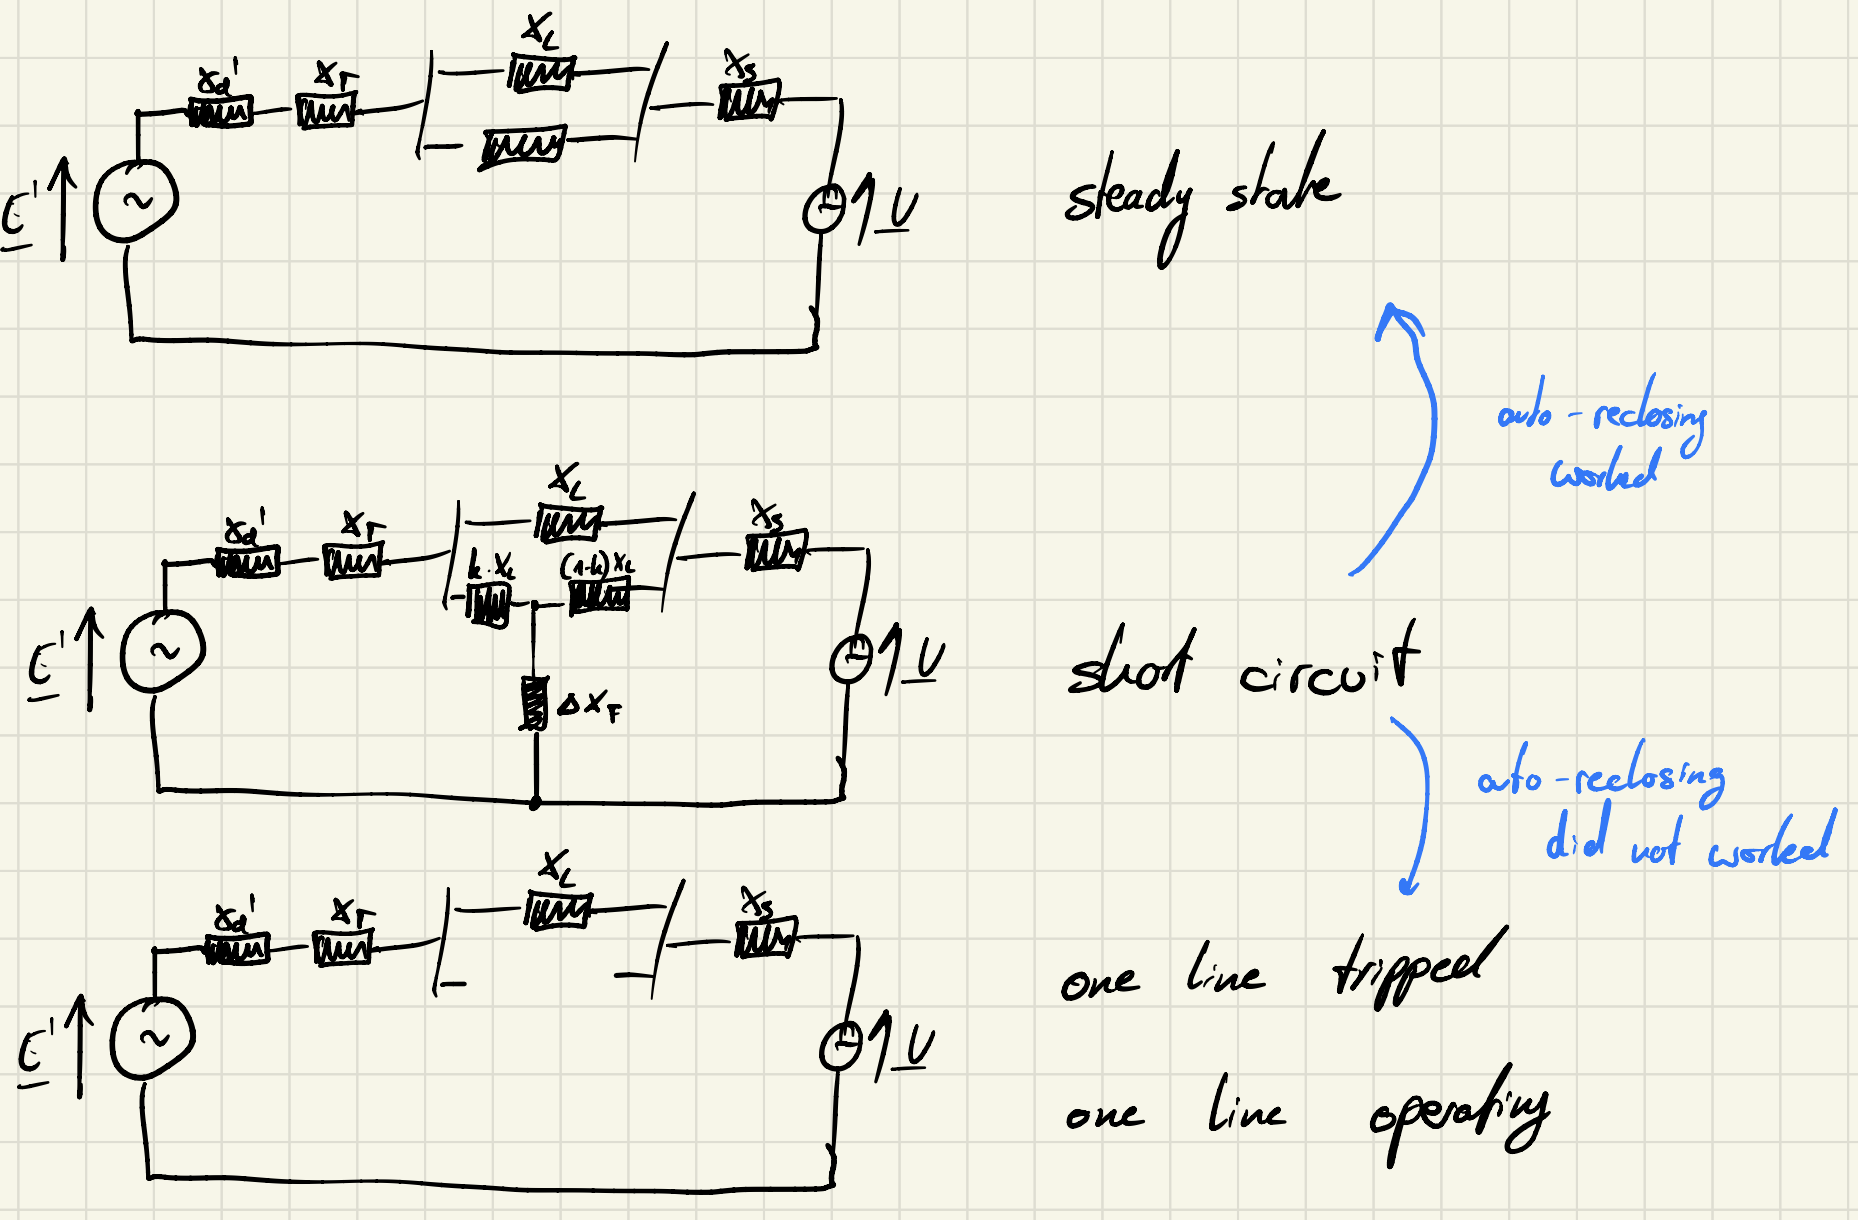
\includegraphics[width=.7\textwidth]{images/electrical_networks.png}
        \caption[Electrical networks for simulation]{Electrical networks for simulation}
        \label{fig:el-networks}
\end{figure}

\autoref{fig:el-networks} shows the steady state circuit, the system during the fault and the possible network after and with no clearing of the fault. Normally the third state is not necessary. The networks in \autoref{fig:simplified-networks} are the represented ones in the simulation, the reactances thus have to be simplified for a targeted simulation.

\begin{figure}[H]
        \centering
        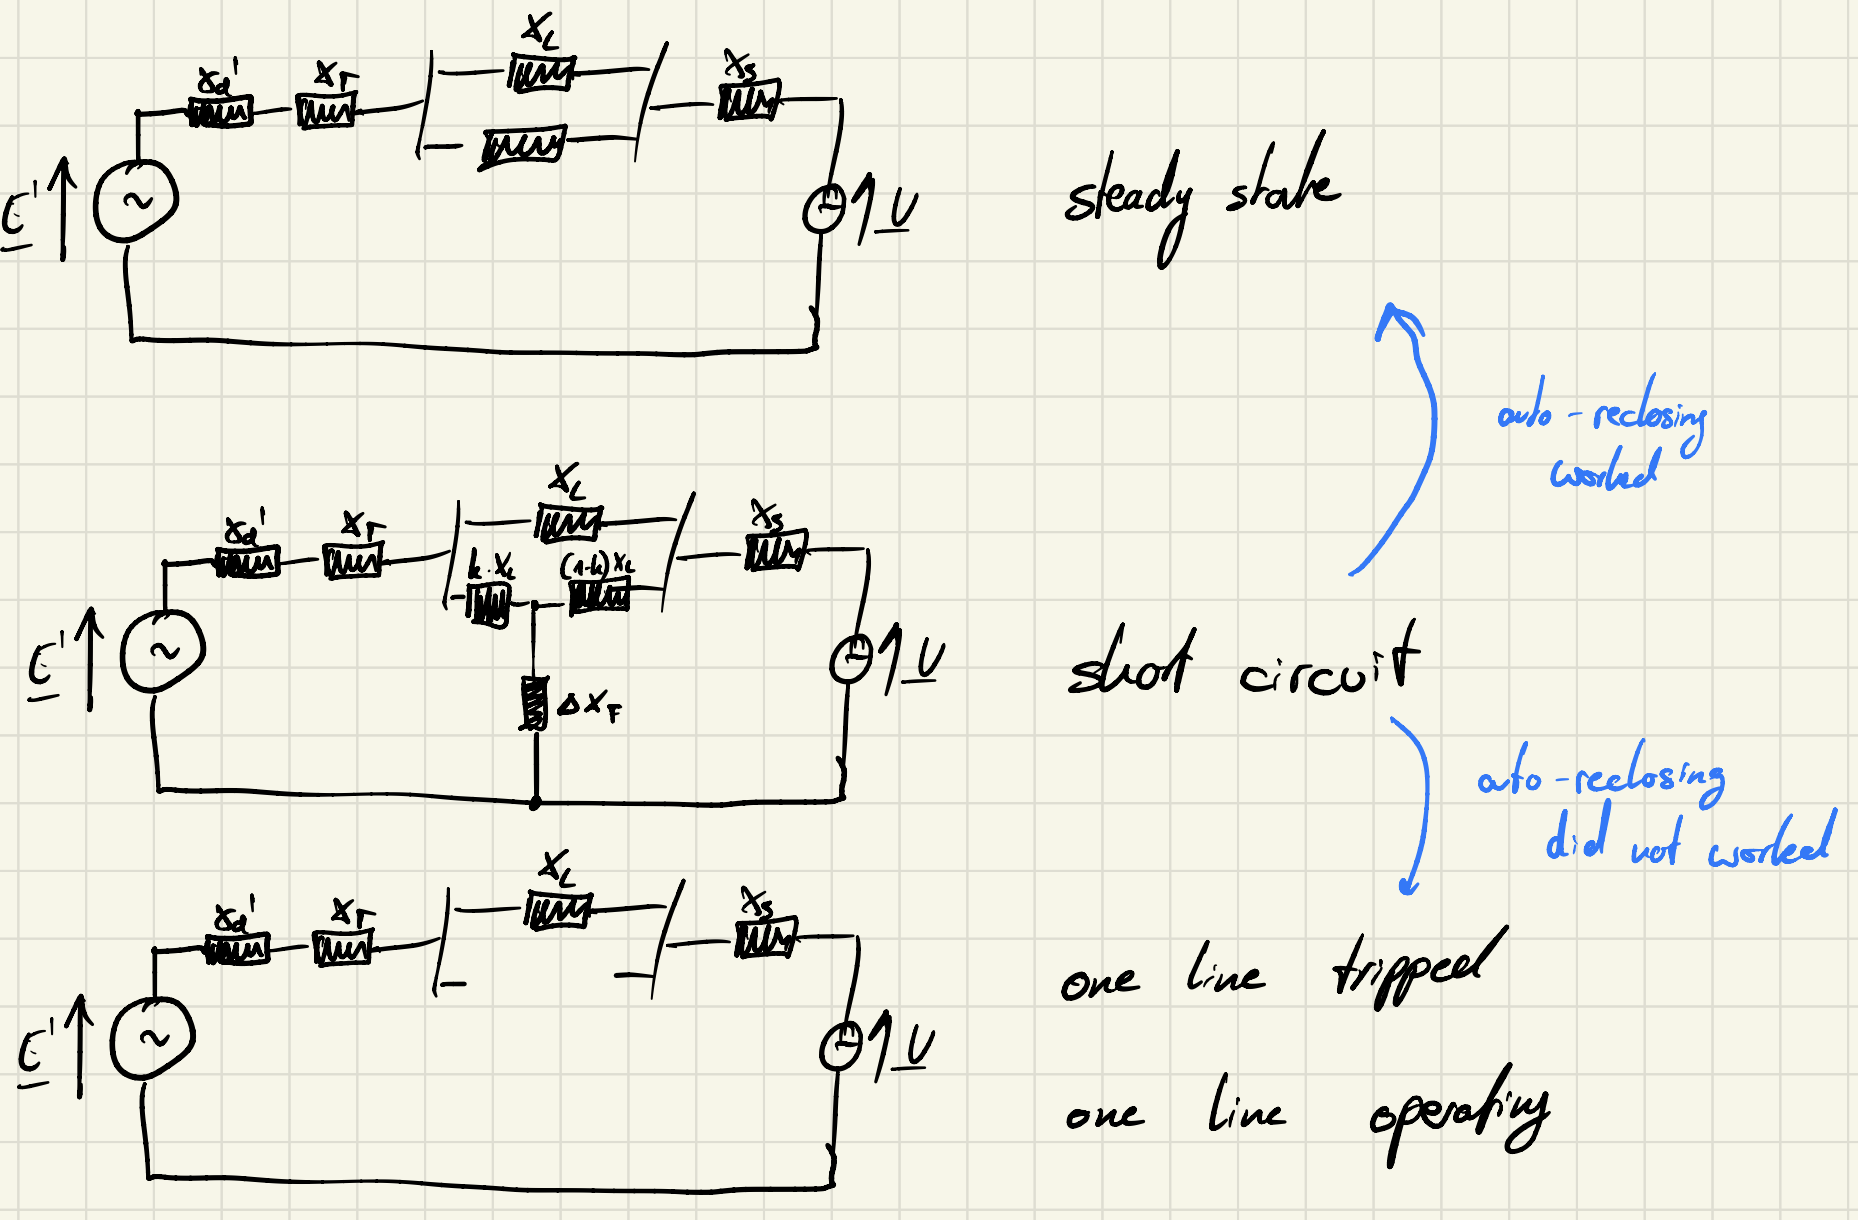
\includegraphics[width=.7\textwidth]{images/electrical_networks.png}
        \caption[Simplified electrical networks]{Simplified electrical networks}
        \label{fig:simplified-networks}
\end{figure}

Electically speaking from the swing equation (\autoref{eq:swing2}), the real power flowing from the \acs{SG} to the \acs{IBB} is to be calculated. With the general equation for the power looking at the generator bus bar
\begin{align}
        P=V \cdot I^* \nonumber,
\end{align}
and ohms law connected with the nodal admittance matrix for the voltage at the bus bar (see \autoref{eq:i-bb} and \ref{eq:vbb}), the only thing left for calculating the power is the injected current from the \acs{SG} to the generator bus bar. The details we know about the \acs{SG} help to decribe it as a voltage source, but with a transformation it can be used as current source, delivering the injected current at the generator bus bar (see \autoref{eq:i-inj}).
\begin{align}
        I_\mathrm{inj}=&~\frac{\underline{E}}{jX} \label{eq:i-inj} \\[6pt]
        V_\mathrm{bb}=&~Y_\mathrm{11} \cdot I_\mathrm{inj,~gen} + Y_\mathrm{12} \cdot I_\mathrm{inj,~ibb} \label{eq:vbb} \\[6pt]
        I_\mathrm{bb}=&~\frac{\underline{E}_\mathrm{gen}-V_\mathrm{bb}}{jX} \label{eq:i-bb}
\end{align}
where

\begin{tabularx}{\textwidth}[H]{lX}
        $\delta$                        & power angle (difference) \\
        $E_\mathrm{p}$                  & pole voltage of the \acf{SG} \\
        % $\underline{E}_\mathrm{T}'$     & complex potential on the primary side of the transformer \\
        % $\underline{E}_\mathrm{T}''$    & complex potential on the secondary side of the transformer \\
        % $\underline{E}_\mathrm{ibb}$    & complex pole potential of the \acf{IBB} \\
        $X_\mathrm{g}'$                 & reactance of the \acf{SG} \\
        $X_\mathrm{l}$                  & reactance of a single line \\
        $X_\mathrm{ibb}$                  & reactance of the \acf{IBB} \\
\end{tabularx}


\subsection{Simulation cases and boundaries}
\label{sec:sim-boundaries}

The boundaries of the single cases, which are simulated, are given with a Python dictionary. Therefore the values of the variables have to be predefined and documented. Considering fault cases, there are three differences in the interest:
\begin{enumerate}
        \item A full line fault, meaning the complete electrical power is disconnected. The \acs{CCT} of the fault has to be determined, a \acs{TDS} with fault clearing shortly before and after the critical clearing is carried out and displayed as {\itshape stable} and {\itshape unstable};
        \item A partial line fault, meaning just a defined percentage of the electrical power is disconnected. The further evaluation is carried out like in scenario 1.;
        \item A partial line fault, meaning just a defined percentage of the electrical power is disconnected. But with consideration, that the fault condition is stable at a new operation point. This point is calculated in the time domain.
\end{enumerate}
Further of interest is a parameter variation of both influences $H_\mathrm{gen}$ and $\Delta P$. This last parameter is not meant to describe the absolute power difference, which is inserted into the swing equation, but more the power difference relative to the maximum electrical power output of the generator. Due to the relation between the maximum power output and the disconnected electrical power in the acceleration and deceleration of the rotor, it seems more significant to use this as a relative parameter. The \acs{CCT} in dependency of these two influences shall be elaborated.

\subsection{Initial value calculation}
\label{sec:initials}

For the setting of starting values, the per unit system is preferred. Because of the relative nature of this unit, it acts as generalization and can be applied to concrete examples with known nominal sizes. Generally speaking, $P_\mathrm{e,max}$, $P_\mathrm{e}=P_\mathrm{mech}$, $E_\mathrm{ibb}$, $E_\mathrm{gen}$, $\delta_\mathrm{ibb}$ and $\delta_\mathrm{gen}$ are needed to be predefined for the simulation. 

As the point of interest in most calculations, the voltage at the at the \acs{IBB} is set to $1~\mathrm{p.u.}$. Most of the until now presented equations are referring to power angle differences. For a simplified calculation, it is handsome to set the power angle of the \acs{IBB} to $0^\circ$, thus all the power angle and angle developments dependent on the time are solely related to the absolute power angle of the generator. The maximum electrical power of the generator is arbitrarily set to $1.2~\mathrm{p.u.}$, the real power extracted from the generator into the grid node is set to $0.9~\mathrm{p.u.}$. With these predefinitions and both following equations we can calculate the remaining two values.
\begin{align}
        E_\mathrm{gen}=&~\frac{P_\mathrm{e,max} \cdot X}{E_\mathrm{ibb} \cdot sin(90^\circ)} \approx 1.14~\mathrm{p.u.} \nonumber \\[6pt]
        \delta_\mathrm{gen}=&~arcsin\Bigg(\frac{P_\mathrm{e} \cdot X}{E_\mathrm{ibb} \cdot E_\mathrm{gen}}\Bigg) \approx 48.6^\circ \nonumber
\end{align}

The reactances for the different fault scenarios can be derived from the electrical networks in \autoref{sec:el-networks}. Therefore the general reactance in operation mode is constituted with the reactance of the generator, the line, and the \acs{IBB}. For fault 1 the additional fault reactance is getting very high in addition to the generator, thus it can be neglected. Fault 2, considering just a partial line tripping, is increasing the contribution from the line to $\frac{3}{2}$ of its initial value. The other contributions stay consistent. For fault scenario 3 the reactances are consistent whether the fault is present or not. The initial electrical power is reduced to  $0.6~\mathrm{p.u.}$ and thus the initial power angle of the generator is set to $30^\circ$\mycomment[MK]{delta berechnen}.

A compromised overview of the initial values and the values in the fault cases is given in \autoref{app:initials}.

%%%%%%%%%%%%%%%%%%%%%%%%%%%%%%%
\section{Implementation of the time domain solution}
\label{sec:tds}

The \acs{TDS} shall be solved with a python integrated solver, due to the fact that numerical solvin methods are not scope of this paper. The solver {\itshape odeint()} from the {\itshape scipy}-package is therefore used as preferred algorithm. This requires a time array with all the timesteps of interest and a differential function, which is solved through every time step. Due to the second order nature of the swing-equation and just the possibility to solve first order ones, the equation has to be split up into two first order equations and solved simultaneously. This can be realized via using a solution array instead of a variable. 

Looking deeper into the swing equation, both the demanded electrical power from the grid or connected network and the mechanical power put into the roter from the steam turbine have to be calculated at each time step. While the mechnanical power is a bit easier to calculate, \mycomment[MK]{Include the equation for the mechanical power?}
% \begin{align}
%         P_\mathrm{m}=P, \nonumber
% \end{align}
the electrical power is a bit more complex. In order to get a good representation, the algebraic equations describing the connected network (see \autoref{sec:el-networks}), have to be solved at every time step as well. For this a dedicated function {\itshape algebraic()} is included.

% \lstinputlisting[caption={Main functions for the \acf{TDS} of the swing equation and \acf{SMIB} model\\}, captionpos=t, style=style-python, label=lst:eac]{python/paper/tds.py}

%%%%%%%%%%%%%%%%%%%%%%%%%%%%%%%
\section{Implementation of the equal area criterion}
\label{sec:eac}

% \commenting{
%         \begin{itemize}
%                 \item Iterative process needed? Due to omega and delta dependencies of $P_e$ and $P_m$
%                 \item Different methods of CCT calculation: P-$\delta$-curve; P-t-curves
%         \end{itemize}
% }

The \acf{EAC} is computed as the name states. It is comparing the accelerated area with the decelerable area, and therefore comparing the stored to the braking (or re-synchronizing) energy. The main function {\itshape deteming\_cct()} is differentiating between clearing and non-clearing mode. First one is taking the pre-fault status of the connected network also as post-fault condition, thus calculating the clearing time and angle the generatr and the network can remain in the fault state. The non-clearing mode is taking the fault condition as post-fault condition and is calculating a new stable power angle convergent.

% \lstinputlisting[caption={Main functions for the determination of the \acf{CCT} with the \acf{EAC}\\}, captionpos=t, style=style-python, label=lst:eac]{python/paper/eac.py}

The main though is iterating through the \acs{TDS} at each time step, looking if enough braking reserve is left and saving the current time and angle as solution. If the loop continues, the solution is overwritten. As pre-set the solution is negative. This enables a quick understanding of simulation faults or a general unstable initial condition set.

As a helping function {\itshape stability\_eac()} allows a simple check in the loop. It calculates the currently passed acceleration area, and the until the maximum dynamically stable power angle $\delta_\mathrm{max}=\pi-\delta_\mathrm{0}$ possible decelerating area, it can compare and state stability or instability at the current time point.

% \commenting{Further functions: Power calculation?}

Another possible way would be to check the stability first under the $P-\delta$-curve, gathering the critical angle. After that a simple run through the \acs{TDS} can deliver the searched \acs{CCT}. Within this approach the angle spectrum has to be searched in addition to the \acs{TDS}. This doubled vector searching seemed as easy improvement in comparison to the previous method and was therefore neglected.

%%%%%%%%%%%%%%%%%%%%%%%%%%%%%%%
%%%%%%%%%%%%%%%%%%%%%%%%%%%%%%%
\chapter{Results}
\label{chap:results}

%%%%%%%%%%%%%%%%%%%%%%%%%%%%%%%
\section{Analytical results}
\label{sec:analytical-results}

\begin{wraptable}{r}{8cm}
        \vspace{-12pt}
        \small
        \centering
        \caption[Analytical results for the two clearing fault-scenarios]{Analytical results for the two clearing fault-scenarios; considering $\delta_\mathrm{cc}$ and $t_\mathrm{cc}$}
        \label{tab:res-analytical}
        \vspace{12pt}
        \begin{tabular}{|l|r|r|}
                \hline
                \rowcolor{lightgray} scenario & $\delta_\mathrm{cc}$ & $t_\mathrm{cc}$  \\ \hline \hline
                fault 1              & 65.01$^\circ$        & 0.116 s                         \\ \hline
                fault 2              & 93.99$^\circ$        & 0.595 s \\ \hline
        \end{tabular}
\end{wraptable}
The analytical calculation follows the equations from \autoref{sec:analytical-method}. For fault 1 the simplified ones could be used, the more complex and advanced are needed for fault case 2. Therefore the base values for the first two input scenarios are used like in the numerical simulation. For the third one no \acs{CCT} is calculatable, due to the stable nature of the fault scenario. The results of this calculation are shown in \autoref{tab:res-analytical}.

\mycomment[MK]{Was ist mit nicht vollständigen Fehlern? Gleichungen für analytical beschreiben nichts...}

%%%%%%%%%%%%%%%%%%%%%%%%%%%%%%%
\section{Numerical results}

\begin{wraptable}{r}{8cm}
        \vspace{-12pt}
        \small
        \centering
        \caption[Numerical results for \acs{CCT}-calculations]{Results (\acs{CCT} and $\delta_\mathrm{cc}$) for numerical solving the faults 1, 2, and 3}
        \label{tab:numerical-solutions}
        \vspace{12pt}
        \begin{tabular}{|l|r|r|}
                \hline
                \rowcolor{lightgray} scenario & $\delta_\mathrm{cc}$ & $t_\mathrm{cc}$ \\ \hline \hline
                fault 1                       & 65.9$^\circ$          & 0.119 s                     \\ \hline
                fault 2                       & 95.9$^\circ$          & 0.394 s                     \\ \hline
        \end{tabular}
\end{wraptable}
\autoref{tab:numerical-solutions} is summarizing the results for the \acs{CCT}-calculation of the different set scenarios in \autoref{sec:scenario}. Like in the anayltical results section before, the third fault can not be displayed in the context of the first two clearing ones. The maximum reached power angle for fault 3 is $69.3^\circ$, while the new stable power angle is around $48.6^\circ$. At first the system oszillates around this new angle, until the damping factor results in a new stable and steady operation point.

\subsection{Simulated faults}

Looking deeper into the numerical results is possible through plotting the development of the power angle over the time. In addition to that the used energies or respectively areas in the $P-\delta$-curves. \autoref{fig:fault3} is looking deeper into the non-clearing fault three. Because of spacial reasons, the complete plot sets for all faults are included in the \autoref{app:fault1}, \autoref{app:fault2} and \autoref{app:fault3}.

\begin{figure}[H]
        \centering
        %% Creator: Matplotlib, PGF backend
%%
%% To include the figure in your LaTeX document, write
%%   \input{<filename>.pgf}
%%
%% Make sure the required packages are loaded in your preamble
%%   \usepackage{pgf}
%%
%% Also ensure that all the required font packages are loaded; for instance,
%% the lmodern package is sometimes necessary when using math font.
%%   \usepackage{lmodern}
%%
%% Figures using additional raster images can only be included by \input if
%% they are in the same directory as the main LaTeX file. For loading figures
%% from other directories you can use the `import` package
%%   \usepackage{import}
%%
%% and then include the figures with
%%   \import{<path to file>}{<filename>.pgf}
%%
%% Matplotlib used the following preamble
%%   
%%   \usepackage{fontspec}
%%   \setmainfont{Charter.ttc}[Path=\detokenize{/System/Library/Fonts/Supplemental/}]
%%   \setsansfont{DejaVuSans.ttf}[Path=\detokenize{/opt/homebrew/lib/python3.10/site-packages/matplotlib/mpl-data/fonts/ttf/}]
%%   \setmonofont{DejaVuSansMono.ttf}[Path=\detokenize{/opt/homebrew/lib/python3.10/site-packages/matplotlib/mpl-data/fonts/ttf/}]
%%   \makeatletter\@ifpackageloaded{underscore}{}{\usepackage[strings]{underscore}}\makeatother
%%
\begingroup%
\makeatletter%
\begin{pgfpicture}%
\pgfpathrectangle{\pgfpointorigin}{\pgfqpoint{5.000000in}{6.000000in}}%
\pgfusepath{use as bounding box, clip}%
\begin{pgfscope}%
\pgfsetbuttcap%
\pgfsetmiterjoin%
\definecolor{currentfill}{rgb}{1.000000,1.000000,1.000000}%
\pgfsetfillcolor{currentfill}%
\pgfsetlinewidth{0.000000pt}%
\definecolor{currentstroke}{rgb}{1.000000,1.000000,1.000000}%
\pgfsetstrokecolor{currentstroke}%
\pgfsetdash{}{0pt}%
\pgfpathmoveto{\pgfqpoint{0.000000in}{0.000000in}}%
\pgfpathlineto{\pgfqpoint{5.000000in}{0.000000in}}%
\pgfpathlineto{\pgfqpoint{5.000000in}{6.000000in}}%
\pgfpathlineto{\pgfqpoint{0.000000in}{6.000000in}}%
\pgfpathlineto{\pgfqpoint{0.000000in}{0.000000in}}%
\pgfpathclose%
\pgfusepath{fill}%
\end{pgfscope}%
\begin{pgfscope}%
\pgfsetbuttcap%
\pgfsetmiterjoin%
\definecolor{currentfill}{rgb}{1.000000,1.000000,1.000000}%
\pgfsetfillcolor{currentfill}%
\pgfsetlinewidth{0.000000pt}%
\definecolor{currentstroke}{rgb}{0.000000,0.000000,0.000000}%
\pgfsetstrokecolor{currentstroke}%
\pgfsetstrokeopacity{0.000000}%
\pgfsetdash{}{0pt}%
\pgfpathmoveto{\pgfqpoint{0.625000in}{2.970000in}}%
\pgfpathlineto{\pgfqpoint{4.500000in}{2.970000in}}%
\pgfpathlineto{\pgfqpoint{4.500000in}{5.280000in}}%
\pgfpathlineto{\pgfqpoint{0.625000in}{5.280000in}}%
\pgfpathlineto{\pgfqpoint{0.625000in}{2.970000in}}%
\pgfpathclose%
\pgfusepath{fill}%
\end{pgfscope}%
\begin{pgfscope}%
\pgfpathrectangle{\pgfqpoint{0.625000in}{2.970000in}}{\pgfqpoint{3.875000in}{2.310000in}}%
\pgfusepath{clip}%
\pgfsetbuttcap%
\pgfsetroundjoin%
\definecolor{currentfill}{rgb}{0.900000,0.900000,0.900000}%
\pgfsetfillcolor{currentfill}%
\pgfsetlinewidth{1.003750pt}%
\definecolor{currentstroke}{rgb}{0.500000,0.500000,0.500000}%
\pgfsetstrokecolor{currentstroke}%
\pgfsetdash{}{0pt}%
\pgfsys@defobject{currentmarker}{\pgfqpoint{1.270833in}{3.710708in}}{\pgfqpoint{1.672006in}{4.081826in}}{%
\pgfpathmoveto{\pgfqpoint{1.270833in}{4.070565in}}%
\pgfpathlineto{\pgfqpoint{1.270833in}{3.710708in}}%
\pgfpathlineto{\pgfqpoint{1.279021in}{3.719207in}}%
\pgfpathlineto{\pgfqpoint{1.287208in}{3.727673in}}%
\pgfpathlineto{\pgfqpoint{1.295395in}{3.736106in}}%
\pgfpathlineto{\pgfqpoint{1.303582in}{3.744505in}}%
\pgfpathlineto{\pgfqpoint{1.311769in}{3.752870in}}%
\pgfpathlineto{\pgfqpoint{1.319956in}{3.761201in}}%
\pgfpathlineto{\pgfqpoint{1.328144in}{3.769497in}}%
\pgfpathlineto{\pgfqpoint{1.336331in}{3.777757in}}%
\pgfpathlineto{\pgfqpoint{1.344518in}{3.785982in}}%
\pgfpathlineto{\pgfqpoint{1.352705in}{3.794171in}}%
\pgfpathlineto{\pgfqpoint{1.360892in}{3.802324in}}%
\pgfpathlineto{\pgfqpoint{1.369080in}{3.810440in}}%
\pgfpathlineto{\pgfqpoint{1.377267in}{3.818518in}}%
\pgfpathlineto{\pgfqpoint{1.385454in}{3.826560in}}%
\pgfpathlineto{\pgfqpoint{1.393641in}{3.834564in}}%
\pgfpathlineto{\pgfqpoint{1.401828in}{3.842530in}}%
\pgfpathlineto{\pgfqpoint{1.410016in}{3.850457in}}%
\pgfpathlineto{\pgfqpoint{1.418203in}{3.858345in}}%
\pgfpathlineto{\pgfqpoint{1.426390in}{3.866195in}}%
\pgfpathlineto{\pgfqpoint{1.434577in}{3.874004in}}%
\pgfpathlineto{\pgfqpoint{1.442764in}{3.881775in}}%
\pgfpathlineto{\pgfqpoint{1.450951in}{3.889504in}}%
\pgfpathlineto{\pgfqpoint{1.459139in}{3.897194in}}%
\pgfpathlineto{\pgfqpoint{1.467326in}{3.904842in}}%
\pgfpathlineto{\pgfqpoint{1.475513in}{3.912450in}}%
\pgfpathlineto{\pgfqpoint{1.483700in}{3.920015in}}%
\pgfpathlineto{\pgfqpoint{1.491887in}{3.927539in}}%
\pgfpathlineto{\pgfqpoint{1.500075in}{3.935021in}}%
\pgfpathlineto{\pgfqpoint{1.508262in}{3.942460in}}%
\pgfpathlineto{\pgfqpoint{1.516449in}{3.949857in}}%
\pgfpathlineto{\pgfqpoint{1.524636in}{3.957210in}}%
\pgfpathlineto{\pgfqpoint{1.532823in}{3.964520in}}%
\pgfpathlineto{\pgfqpoint{1.541011in}{3.971785in}}%
\pgfpathlineto{\pgfqpoint{1.549198in}{3.979007in}}%
\pgfpathlineto{\pgfqpoint{1.557385in}{3.986185in}}%
\pgfpathlineto{\pgfqpoint{1.565572in}{3.993317in}}%
\pgfpathlineto{\pgfqpoint{1.573759in}{4.000405in}}%
\pgfpathlineto{\pgfqpoint{1.581946in}{4.007447in}}%
\pgfpathlineto{\pgfqpoint{1.590134in}{4.014443in}}%
\pgfpathlineto{\pgfqpoint{1.598321in}{4.021393in}}%
\pgfpathlineto{\pgfqpoint{1.606508in}{4.028297in}}%
\pgfpathlineto{\pgfqpoint{1.614695in}{4.035155in}}%
\pgfpathlineto{\pgfqpoint{1.622882in}{4.041965in}}%
\pgfpathlineto{\pgfqpoint{1.631070in}{4.048728in}}%
\pgfpathlineto{\pgfqpoint{1.639257in}{4.055444in}}%
\pgfpathlineto{\pgfqpoint{1.647444in}{4.062112in}}%
\pgfpathlineto{\pgfqpoint{1.655631in}{4.068732in}}%
\pgfpathlineto{\pgfqpoint{1.663818in}{4.075303in}}%
\pgfpathlineto{\pgfqpoint{1.672006in}{4.081826in}}%
\pgfpathlineto{\pgfqpoint{1.672006in}{4.070565in}}%
\pgfpathlineto{\pgfqpoint{1.672006in}{4.070565in}}%
\pgfpathlineto{\pgfqpoint{1.663818in}{4.070565in}}%
\pgfpathlineto{\pgfqpoint{1.655631in}{4.070565in}}%
\pgfpathlineto{\pgfqpoint{1.647444in}{4.070565in}}%
\pgfpathlineto{\pgfqpoint{1.639257in}{4.070565in}}%
\pgfpathlineto{\pgfqpoint{1.631070in}{4.070565in}}%
\pgfpathlineto{\pgfqpoint{1.622882in}{4.070565in}}%
\pgfpathlineto{\pgfqpoint{1.614695in}{4.070565in}}%
\pgfpathlineto{\pgfqpoint{1.606508in}{4.070565in}}%
\pgfpathlineto{\pgfqpoint{1.598321in}{4.070565in}}%
\pgfpathlineto{\pgfqpoint{1.590134in}{4.070565in}}%
\pgfpathlineto{\pgfqpoint{1.581946in}{4.070565in}}%
\pgfpathlineto{\pgfqpoint{1.573759in}{4.070565in}}%
\pgfpathlineto{\pgfqpoint{1.565572in}{4.070565in}}%
\pgfpathlineto{\pgfqpoint{1.557385in}{4.070565in}}%
\pgfpathlineto{\pgfqpoint{1.549198in}{4.070565in}}%
\pgfpathlineto{\pgfqpoint{1.541011in}{4.070565in}}%
\pgfpathlineto{\pgfqpoint{1.532823in}{4.070565in}}%
\pgfpathlineto{\pgfqpoint{1.524636in}{4.070565in}}%
\pgfpathlineto{\pgfqpoint{1.516449in}{4.070565in}}%
\pgfpathlineto{\pgfqpoint{1.508262in}{4.070565in}}%
\pgfpathlineto{\pgfqpoint{1.500075in}{4.070565in}}%
\pgfpathlineto{\pgfqpoint{1.491887in}{4.070565in}}%
\pgfpathlineto{\pgfqpoint{1.483700in}{4.070565in}}%
\pgfpathlineto{\pgfqpoint{1.475513in}{4.070565in}}%
\pgfpathlineto{\pgfqpoint{1.467326in}{4.070565in}}%
\pgfpathlineto{\pgfqpoint{1.459139in}{4.070565in}}%
\pgfpathlineto{\pgfqpoint{1.450951in}{4.070565in}}%
\pgfpathlineto{\pgfqpoint{1.442764in}{4.070565in}}%
\pgfpathlineto{\pgfqpoint{1.434577in}{4.070565in}}%
\pgfpathlineto{\pgfqpoint{1.426390in}{4.070565in}}%
\pgfpathlineto{\pgfqpoint{1.418203in}{4.070565in}}%
\pgfpathlineto{\pgfqpoint{1.410016in}{4.070565in}}%
\pgfpathlineto{\pgfqpoint{1.401828in}{4.070565in}}%
\pgfpathlineto{\pgfqpoint{1.393641in}{4.070565in}}%
\pgfpathlineto{\pgfqpoint{1.385454in}{4.070565in}}%
\pgfpathlineto{\pgfqpoint{1.377267in}{4.070565in}}%
\pgfpathlineto{\pgfqpoint{1.369080in}{4.070565in}}%
\pgfpathlineto{\pgfqpoint{1.360892in}{4.070565in}}%
\pgfpathlineto{\pgfqpoint{1.352705in}{4.070565in}}%
\pgfpathlineto{\pgfqpoint{1.344518in}{4.070565in}}%
\pgfpathlineto{\pgfqpoint{1.336331in}{4.070565in}}%
\pgfpathlineto{\pgfqpoint{1.328144in}{4.070565in}}%
\pgfpathlineto{\pgfqpoint{1.319956in}{4.070565in}}%
\pgfpathlineto{\pgfqpoint{1.311769in}{4.070565in}}%
\pgfpathlineto{\pgfqpoint{1.303582in}{4.070565in}}%
\pgfpathlineto{\pgfqpoint{1.295395in}{4.070565in}}%
\pgfpathlineto{\pgfqpoint{1.287208in}{4.070565in}}%
\pgfpathlineto{\pgfqpoint{1.279021in}{4.070565in}}%
\pgfpathlineto{\pgfqpoint{1.270833in}{4.070565in}}%
\pgfpathlineto{\pgfqpoint{1.270833in}{4.070565in}}%
\pgfpathclose%
\pgfusepath{stroke,fill}%
}%
\begin{pgfscope}%
\pgfsys@transformshift{0.000000in}{0.000000in}%
\pgfsys@useobject{currentmarker}{}%
\end{pgfscope}%
\end{pgfscope}%
\begin{pgfscope}%
\pgfpathrectangle{\pgfqpoint{0.625000in}{2.970000in}}{\pgfqpoint{3.875000in}{2.310000in}}%
\pgfusepath{clip}%
\pgfsetbuttcap%
\pgfsetroundjoin%
\definecolor{currentfill}{rgb}{0.900000,0.900000,0.900000}%
\pgfsetfillcolor{currentfill}%
\pgfsetlinewidth{1.003750pt}%
\definecolor{currentstroke}{rgb}{0.500000,0.500000,0.500000}%
\pgfsetstrokecolor{currentstroke}%
\pgfsetdash{}{0pt}%
\pgfsys@defobject{currentmarker}{\pgfqpoint{1.672006in}{4.070565in}}{\pgfqpoint{2.116048in}{4.355429in}}{%
\pgfpathmoveto{\pgfqpoint{1.672006in}{4.070565in}}%
\pgfpathlineto{\pgfqpoint{1.672006in}{4.081826in}}%
\pgfpathlineto{\pgfqpoint{1.681068in}{4.088988in}}%
\pgfpathlineto{\pgfqpoint{1.690130in}{4.096090in}}%
\pgfpathlineto{\pgfqpoint{1.699192in}{4.103132in}}%
\pgfpathlineto{\pgfqpoint{1.708254in}{4.110112in}}%
\pgfpathlineto{\pgfqpoint{1.717316in}{4.117031in}}%
\pgfpathlineto{\pgfqpoint{1.726378in}{4.123887in}}%
\pgfpathlineto{\pgfqpoint{1.735440in}{4.130682in}}%
\pgfpathlineto{\pgfqpoint{1.744502in}{4.137414in}}%
\pgfpathlineto{\pgfqpoint{1.753564in}{4.144083in}}%
\pgfpathlineto{\pgfqpoint{1.762626in}{4.150688in}}%
\pgfpathlineto{\pgfqpoint{1.771689in}{4.157230in}}%
\pgfpathlineto{\pgfqpoint{1.780751in}{4.163707in}}%
\pgfpathlineto{\pgfqpoint{1.789813in}{4.170121in}}%
\pgfpathlineto{\pgfqpoint{1.798875in}{4.176469in}}%
\pgfpathlineto{\pgfqpoint{1.807937in}{4.182752in}}%
\pgfpathlineto{\pgfqpoint{1.816999in}{4.188970in}}%
\pgfpathlineto{\pgfqpoint{1.826061in}{4.195122in}}%
\pgfpathlineto{\pgfqpoint{1.835123in}{4.201208in}}%
\pgfpathlineto{\pgfqpoint{1.844185in}{4.207227in}}%
\pgfpathlineto{\pgfqpoint{1.853247in}{4.213180in}}%
\pgfpathlineto{\pgfqpoint{1.862309in}{4.219066in}}%
\pgfpathlineto{\pgfqpoint{1.871371in}{4.224884in}}%
\pgfpathlineto{\pgfqpoint{1.880434in}{4.230634in}}%
\pgfpathlineto{\pgfqpoint{1.889496in}{4.236317in}}%
\pgfpathlineto{\pgfqpoint{1.898558in}{4.241931in}}%
\pgfpathlineto{\pgfqpoint{1.907620in}{4.247476in}}%
\pgfpathlineto{\pgfqpoint{1.916682in}{4.252952in}}%
\pgfpathlineto{\pgfqpoint{1.925744in}{4.258359in}}%
\pgfpathlineto{\pgfqpoint{1.934806in}{4.263697in}}%
\pgfpathlineto{\pgfqpoint{1.943868in}{4.268965in}}%
\pgfpathlineto{\pgfqpoint{1.952930in}{4.274162in}}%
\pgfpathlineto{\pgfqpoint{1.961992in}{4.279290in}}%
\pgfpathlineto{\pgfqpoint{1.971054in}{4.284346in}}%
\pgfpathlineto{\pgfqpoint{1.980117in}{4.289332in}}%
\pgfpathlineto{\pgfqpoint{1.989179in}{4.294246in}}%
\pgfpathlineto{\pgfqpoint{1.998241in}{4.299089in}}%
\pgfpathlineto{\pgfqpoint{2.007303in}{4.303861in}}%
\pgfpathlineto{\pgfqpoint{2.016365in}{4.308560in}}%
\pgfpathlineto{\pgfqpoint{2.025427in}{4.313187in}}%
\pgfpathlineto{\pgfqpoint{2.034489in}{4.317741in}}%
\pgfpathlineto{\pgfqpoint{2.043551in}{4.322223in}}%
\pgfpathlineto{\pgfqpoint{2.052613in}{4.326632in}}%
\pgfpathlineto{\pgfqpoint{2.061675in}{4.330967in}}%
\pgfpathlineto{\pgfqpoint{2.070737in}{4.335229in}}%
\pgfpathlineto{\pgfqpoint{2.079800in}{4.339417in}}%
\pgfpathlineto{\pgfqpoint{2.088862in}{4.343532in}}%
\pgfpathlineto{\pgfqpoint{2.097924in}{4.347572in}}%
\pgfpathlineto{\pgfqpoint{2.106986in}{4.351538in}}%
\pgfpathlineto{\pgfqpoint{2.116048in}{4.355429in}}%
\pgfpathlineto{\pgfqpoint{2.116048in}{4.070565in}}%
\pgfpathlineto{\pgfqpoint{2.116048in}{4.070565in}}%
\pgfpathlineto{\pgfqpoint{2.106986in}{4.070565in}}%
\pgfpathlineto{\pgfqpoint{2.097924in}{4.070565in}}%
\pgfpathlineto{\pgfqpoint{2.088862in}{4.070565in}}%
\pgfpathlineto{\pgfqpoint{2.079800in}{4.070565in}}%
\pgfpathlineto{\pgfqpoint{2.070737in}{4.070565in}}%
\pgfpathlineto{\pgfqpoint{2.061675in}{4.070565in}}%
\pgfpathlineto{\pgfqpoint{2.052613in}{4.070565in}}%
\pgfpathlineto{\pgfqpoint{2.043551in}{4.070565in}}%
\pgfpathlineto{\pgfqpoint{2.034489in}{4.070565in}}%
\pgfpathlineto{\pgfqpoint{2.025427in}{4.070565in}}%
\pgfpathlineto{\pgfqpoint{2.016365in}{4.070565in}}%
\pgfpathlineto{\pgfqpoint{2.007303in}{4.070565in}}%
\pgfpathlineto{\pgfqpoint{1.998241in}{4.070565in}}%
\pgfpathlineto{\pgfqpoint{1.989179in}{4.070565in}}%
\pgfpathlineto{\pgfqpoint{1.980117in}{4.070565in}}%
\pgfpathlineto{\pgfqpoint{1.971054in}{4.070565in}}%
\pgfpathlineto{\pgfqpoint{1.961992in}{4.070565in}}%
\pgfpathlineto{\pgfqpoint{1.952930in}{4.070565in}}%
\pgfpathlineto{\pgfqpoint{1.943868in}{4.070565in}}%
\pgfpathlineto{\pgfqpoint{1.934806in}{4.070565in}}%
\pgfpathlineto{\pgfqpoint{1.925744in}{4.070565in}}%
\pgfpathlineto{\pgfqpoint{1.916682in}{4.070565in}}%
\pgfpathlineto{\pgfqpoint{1.907620in}{4.070565in}}%
\pgfpathlineto{\pgfqpoint{1.898558in}{4.070565in}}%
\pgfpathlineto{\pgfqpoint{1.889496in}{4.070565in}}%
\pgfpathlineto{\pgfqpoint{1.880434in}{4.070565in}}%
\pgfpathlineto{\pgfqpoint{1.871371in}{4.070565in}}%
\pgfpathlineto{\pgfqpoint{1.862309in}{4.070565in}}%
\pgfpathlineto{\pgfqpoint{1.853247in}{4.070565in}}%
\pgfpathlineto{\pgfqpoint{1.844185in}{4.070565in}}%
\pgfpathlineto{\pgfqpoint{1.835123in}{4.070565in}}%
\pgfpathlineto{\pgfqpoint{1.826061in}{4.070565in}}%
\pgfpathlineto{\pgfqpoint{1.816999in}{4.070565in}}%
\pgfpathlineto{\pgfqpoint{1.807937in}{4.070565in}}%
\pgfpathlineto{\pgfqpoint{1.798875in}{4.070565in}}%
\pgfpathlineto{\pgfqpoint{1.789813in}{4.070565in}}%
\pgfpathlineto{\pgfqpoint{1.780751in}{4.070565in}}%
\pgfpathlineto{\pgfqpoint{1.771689in}{4.070565in}}%
\pgfpathlineto{\pgfqpoint{1.762626in}{4.070565in}}%
\pgfpathlineto{\pgfqpoint{1.753564in}{4.070565in}}%
\pgfpathlineto{\pgfqpoint{1.744502in}{4.070565in}}%
\pgfpathlineto{\pgfqpoint{1.735440in}{4.070565in}}%
\pgfpathlineto{\pgfqpoint{1.726378in}{4.070565in}}%
\pgfpathlineto{\pgfqpoint{1.717316in}{4.070565in}}%
\pgfpathlineto{\pgfqpoint{1.708254in}{4.070565in}}%
\pgfpathlineto{\pgfqpoint{1.699192in}{4.070565in}}%
\pgfpathlineto{\pgfqpoint{1.690130in}{4.070565in}}%
\pgfpathlineto{\pgfqpoint{1.681068in}{4.070565in}}%
\pgfpathlineto{\pgfqpoint{1.672006in}{4.070565in}}%
\pgfpathlineto{\pgfqpoint{1.672006in}{4.070565in}}%
\pgfpathclose%
\pgfusepath{stroke,fill}%
}%
\begin{pgfscope}%
\pgfsys@transformshift{0.000000in}{0.000000in}%
\pgfsys@useobject{currentmarker}{}%
\end{pgfscope}%
\end{pgfscope}%
\begin{pgfscope}%
\pgfpathrectangle{\pgfqpoint{0.625000in}{2.970000in}}{\pgfqpoint{3.875000in}{2.310000in}}%
\pgfusepath{clip}%
\pgfsetrectcap%
\pgfsetroundjoin%
\pgfsetlinewidth{0.803000pt}%
\definecolor{currentstroke}{rgb}{0.690196,0.690196,0.690196}%
\pgfsetstrokecolor{currentstroke}%
\pgfsetdash{}{0pt}%
\pgfpathmoveto{\pgfqpoint{0.625000in}{2.970000in}}%
\pgfpathlineto{\pgfqpoint{0.625000in}{5.280000in}}%
\pgfusepath{stroke}%
\end{pgfscope}%
\begin{pgfscope}%
\pgfsetbuttcap%
\pgfsetroundjoin%
\definecolor{currentfill}{rgb}{0.000000,0.000000,0.000000}%
\pgfsetfillcolor{currentfill}%
\pgfsetlinewidth{0.803000pt}%
\definecolor{currentstroke}{rgb}{0.000000,0.000000,0.000000}%
\pgfsetstrokecolor{currentstroke}%
\pgfsetdash{}{0pt}%
\pgfsys@defobject{currentmarker}{\pgfqpoint{0.000000in}{-0.048611in}}{\pgfqpoint{0.000000in}{0.000000in}}{%
\pgfpathmoveto{\pgfqpoint{0.000000in}{0.000000in}}%
\pgfpathlineto{\pgfqpoint{0.000000in}{-0.048611in}}%
\pgfusepath{stroke,fill}%
}%
\begin{pgfscope}%
\pgfsys@transformshift{0.625000in}{2.970000in}%
\pgfsys@useobject{currentmarker}{}%
\end{pgfscope}%
\end{pgfscope}%
\begin{pgfscope}%
\pgfpathrectangle{\pgfqpoint{0.625000in}{2.970000in}}{\pgfqpoint{3.875000in}{2.310000in}}%
\pgfusepath{clip}%
\pgfsetrectcap%
\pgfsetroundjoin%
\pgfsetlinewidth{0.803000pt}%
\definecolor{currentstroke}{rgb}{0.690196,0.690196,0.690196}%
\pgfsetstrokecolor{currentstroke}%
\pgfsetdash{}{0pt}%
\pgfpathmoveto{\pgfqpoint{1.055556in}{2.970000in}}%
\pgfpathlineto{\pgfqpoint{1.055556in}{5.280000in}}%
\pgfusepath{stroke}%
\end{pgfscope}%
\begin{pgfscope}%
\pgfsetbuttcap%
\pgfsetroundjoin%
\definecolor{currentfill}{rgb}{0.000000,0.000000,0.000000}%
\pgfsetfillcolor{currentfill}%
\pgfsetlinewidth{0.803000pt}%
\definecolor{currentstroke}{rgb}{0.000000,0.000000,0.000000}%
\pgfsetstrokecolor{currentstroke}%
\pgfsetdash{}{0pt}%
\pgfsys@defobject{currentmarker}{\pgfqpoint{0.000000in}{-0.048611in}}{\pgfqpoint{0.000000in}{0.000000in}}{%
\pgfpathmoveto{\pgfqpoint{0.000000in}{0.000000in}}%
\pgfpathlineto{\pgfqpoint{0.000000in}{-0.048611in}}%
\pgfusepath{stroke,fill}%
}%
\begin{pgfscope}%
\pgfsys@transformshift{1.055556in}{2.970000in}%
\pgfsys@useobject{currentmarker}{}%
\end{pgfscope}%
\end{pgfscope}%
\begin{pgfscope}%
\pgfpathrectangle{\pgfqpoint{0.625000in}{2.970000in}}{\pgfqpoint{3.875000in}{2.310000in}}%
\pgfusepath{clip}%
\pgfsetrectcap%
\pgfsetroundjoin%
\pgfsetlinewidth{0.803000pt}%
\definecolor{currentstroke}{rgb}{0.690196,0.690196,0.690196}%
\pgfsetstrokecolor{currentstroke}%
\pgfsetdash{}{0pt}%
\pgfpathmoveto{\pgfqpoint{1.486111in}{2.970000in}}%
\pgfpathlineto{\pgfqpoint{1.486111in}{5.280000in}}%
\pgfusepath{stroke}%
\end{pgfscope}%
\begin{pgfscope}%
\pgfsetbuttcap%
\pgfsetroundjoin%
\definecolor{currentfill}{rgb}{0.000000,0.000000,0.000000}%
\pgfsetfillcolor{currentfill}%
\pgfsetlinewidth{0.803000pt}%
\definecolor{currentstroke}{rgb}{0.000000,0.000000,0.000000}%
\pgfsetstrokecolor{currentstroke}%
\pgfsetdash{}{0pt}%
\pgfsys@defobject{currentmarker}{\pgfqpoint{0.000000in}{-0.048611in}}{\pgfqpoint{0.000000in}{0.000000in}}{%
\pgfpathmoveto{\pgfqpoint{0.000000in}{0.000000in}}%
\pgfpathlineto{\pgfqpoint{0.000000in}{-0.048611in}}%
\pgfusepath{stroke,fill}%
}%
\begin{pgfscope}%
\pgfsys@transformshift{1.486111in}{2.970000in}%
\pgfsys@useobject{currentmarker}{}%
\end{pgfscope}%
\end{pgfscope}%
\begin{pgfscope}%
\pgfpathrectangle{\pgfqpoint{0.625000in}{2.970000in}}{\pgfqpoint{3.875000in}{2.310000in}}%
\pgfusepath{clip}%
\pgfsetrectcap%
\pgfsetroundjoin%
\pgfsetlinewidth{0.803000pt}%
\definecolor{currentstroke}{rgb}{0.690196,0.690196,0.690196}%
\pgfsetstrokecolor{currentstroke}%
\pgfsetdash{}{0pt}%
\pgfpathmoveto{\pgfqpoint{1.916667in}{2.970000in}}%
\pgfpathlineto{\pgfqpoint{1.916667in}{5.280000in}}%
\pgfusepath{stroke}%
\end{pgfscope}%
\begin{pgfscope}%
\pgfsetbuttcap%
\pgfsetroundjoin%
\definecolor{currentfill}{rgb}{0.000000,0.000000,0.000000}%
\pgfsetfillcolor{currentfill}%
\pgfsetlinewidth{0.803000pt}%
\definecolor{currentstroke}{rgb}{0.000000,0.000000,0.000000}%
\pgfsetstrokecolor{currentstroke}%
\pgfsetdash{}{0pt}%
\pgfsys@defobject{currentmarker}{\pgfqpoint{0.000000in}{-0.048611in}}{\pgfqpoint{0.000000in}{0.000000in}}{%
\pgfpathmoveto{\pgfqpoint{0.000000in}{0.000000in}}%
\pgfpathlineto{\pgfqpoint{0.000000in}{-0.048611in}}%
\pgfusepath{stroke,fill}%
}%
\begin{pgfscope}%
\pgfsys@transformshift{1.916667in}{2.970000in}%
\pgfsys@useobject{currentmarker}{}%
\end{pgfscope}%
\end{pgfscope}%
\begin{pgfscope}%
\pgfpathrectangle{\pgfqpoint{0.625000in}{2.970000in}}{\pgfqpoint{3.875000in}{2.310000in}}%
\pgfusepath{clip}%
\pgfsetrectcap%
\pgfsetroundjoin%
\pgfsetlinewidth{0.803000pt}%
\definecolor{currentstroke}{rgb}{0.690196,0.690196,0.690196}%
\pgfsetstrokecolor{currentstroke}%
\pgfsetdash{}{0pt}%
\pgfpathmoveto{\pgfqpoint{2.347222in}{2.970000in}}%
\pgfpathlineto{\pgfqpoint{2.347222in}{5.280000in}}%
\pgfusepath{stroke}%
\end{pgfscope}%
\begin{pgfscope}%
\pgfsetbuttcap%
\pgfsetroundjoin%
\definecolor{currentfill}{rgb}{0.000000,0.000000,0.000000}%
\pgfsetfillcolor{currentfill}%
\pgfsetlinewidth{0.803000pt}%
\definecolor{currentstroke}{rgb}{0.000000,0.000000,0.000000}%
\pgfsetstrokecolor{currentstroke}%
\pgfsetdash{}{0pt}%
\pgfsys@defobject{currentmarker}{\pgfqpoint{0.000000in}{-0.048611in}}{\pgfqpoint{0.000000in}{0.000000in}}{%
\pgfpathmoveto{\pgfqpoint{0.000000in}{0.000000in}}%
\pgfpathlineto{\pgfqpoint{0.000000in}{-0.048611in}}%
\pgfusepath{stroke,fill}%
}%
\begin{pgfscope}%
\pgfsys@transformshift{2.347222in}{2.970000in}%
\pgfsys@useobject{currentmarker}{}%
\end{pgfscope}%
\end{pgfscope}%
\begin{pgfscope}%
\pgfpathrectangle{\pgfqpoint{0.625000in}{2.970000in}}{\pgfqpoint{3.875000in}{2.310000in}}%
\pgfusepath{clip}%
\pgfsetrectcap%
\pgfsetroundjoin%
\pgfsetlinewidth{0.803000pt}%
\definecolor{currentstroke}{rgb}{0.690196,0.690196,0.690196}%
\pgfsetstrokecolor{currentstroke}%
\pgfsetdash{}{0pt}%
\pgfpathmoveto{\pgfqpoint{2.777778in}{2.970000in}}%
\pgfpathlineto{\pgfqpoint{2.777778in}{5.280000in}}%
\pgfusepath{stroke}%
\end{pgfscope}%
\begin{pgfscope}%
\pgfsetbuttcap%
\pgfsetroundjoin%
\definecolor{currentfill}{rgb}{0.000000,0.000000,0.000000}%
\pgfsetfillcolor{currentfill}%
\pgfsetlinewidth{0.803000pt}%
\definecolor{currentstroke}{rgb}{0.000000,0.000000,0.000000}%
\pgfsetstrokecolor{currentstroke}%
\pgfsetdash{}{0pt}%
\pgfsys@defobject{currentmarker}{\pgfqpoint{0.000000in}{-0.048611in}}{\pgfqpoint{0.000000in}{0.000000in}}{%
\pgfpathmoveto{\pgfqpoint{0.000000in}{0.000000in}}%
\pgfpathlineto{\pgfqpoint{0.000000in}{-0.048611in}}%
\pgfusepath{stroke,fill}%
}%
\begin{pgfscope}%
\pgfsys@transformshift{2.777778in}{2.970000in}%
\pgfsys@useobject{currentmarker}{}%
\end{pgfscope}%
\end{pgfscope}%
\begin{pgfscope}%
\pgfpathrectangle{\pgfqpoint{0.625000in}{2.970000in}}{\pgfqpoint{3.875000in}{2.310000in}}%
\pgfusepath{clip}%
\pgfsetrectcap%
\pgfsetroundjoin%
\pgfsetlinewidth{0.803000pt}%
\definecolor{currentstroke}{rgb}{0.690196,0.690196,0.690196}%
\pgfsetstrokecolor{currentstroke}%
\pgfsetdash{}{0pt}%
\pgfpathmoveto{\pgfqpoint{3.208333in}{2.970000in}}%
\pgfpathlineto{\pgfqpoint{3.208333in}{5.280000in}}%
\pgfusepath{stroke}%
\end{pgfscope}%
\begin{pgfscope}%
\pgfsetbuttcap%
\pgfsetroundjoin%
\definecolor{currentfill}{rgb}{0.000000,0.000000,0.000000}%
\pgfsetfillcolor{currentfill}%
\pgfsetlinewidth{0.803000pt}%
\definecolor{currentstroke}{rgb}{0.000000,0.000000,0.000000}%
\pgfsetstrokecolor{currentstroke}%
\pgfsetdash{}{0pt}%
\pgfsys@defobject{currentmarker}{\pgfqpoint{0.000000in}{-0.048611in}}{\pgfqpoint{0.000000in}{0.000000in}}{%
\pgfpathmoveto{\pgfqpoint{0.000000in}{0.000000in}}%
\pgfpathlineto{\pgfqpoint{0.000000in}{-0.048611in}}%
\pgfusepath{stroke,fill}%
}%
\begin{pgfscope}%
\pgfsys@transformshift{3.208333in}{2.970000in}%
\pgfsys@useobject{currentmarker}{}%
\end{pgfscope}%
\end{pgfscope}%
\begin{pgfscope}%
\pgfpathrectangle{\pgfqpoint{0.625000in}{2.970000in}}{\pgfqpoint{3.875000in}{2.310000in}}%
\pgfusepath{clip}%
\pgfsetrectcap%
\pgfsetroundjoin%
\pgfsetlinewidth{0.803000pt}%
\definecolor{currentstroke}{rgb}{0.690196,0.690196,0.690196}%
\pgfsetstrokecolor{currentstroke}%
\pgfsetdash{}{0pt}%
\pgfpathmoveto{\pgfqpoint{3.638889in}{2.970000in}}%
\pgfpathlineto{\pgfqpoint{3.638889in}{5.280000in}}%
\pgfusepath{stroke}%
\end{pgfscope}%
\begin{pgfscope}%
\pgfsetbuttcap%
\pgfsetroundjoin%
\definecolor{currentfill}{rgb}{0.000000,0.000000,0.000000}%
\pgfsetfillcolor{currentfill}%
\pgfsetlinewidth{0.803000pt}%
\definecolor{currentstroke}{rgb}{0.000000,0.000000,0.000000}%
\pgfsetstrokecolor{currentstroke}%
\pgfsetdash{}{0pt}%
\pgfsys@defobject{currentmarker}{\pgfqpoint{0.000000in}{-0.048611in}}{\pgfqpoint{0.000000in}{0.000000in}}{%
\pgfpathmoveto{\pgfqpoint{0.000000in}{0.000000in}}%
\pgfpathlineto{\pgfqpoint{0.000000in}{-0.048611in}}%
\pgfusepath{stroke,fill}%
}%
\begin{pgfscope}%
\pgfsys@transformshift{3.638889in}{2.970000in}%
\pgfsys@useobject{currentmarker}{}%
\end{pgfscope}%
\end{pgfscope}%
\begin{pgfscope}%
\pgfpathrectangle{\pgfqpoint{0.625000in}{2.970000in}}{\pgfqpoint{3.875000in}{2.310000in}}%
\pgfusepath{clip}%
\pgfsetrectcap%
\pgfsetroundjoin%
\pgfsetlinewidth{0.803000pt}%
\definecolor{currentstroke}{rgb}{0.690196,0.690196,0.690196}%
\pgfsetstrokecolor{currentstroke}%
\pgfsetdash{}{0pt}%
\pgfpathmoveto{\pgfqpoint{4.069444in}{2.970000in}}%
\pgfpathlineto{\pgfqpoint{4.069444in}{5.280000in}}%
\pgfusepath{stroke}%
\end{pgfscope}%
\begin{pgfscope}%
\pgfsetbuttcap%
\pgfsetroundjoin%
\definecolor{currentfill}{rgb}{0.000000,0.000000,0.000000}%
\pgfsetfillcolor{currentfill}%
\pgfsetlinewidth{0.803000pt}%
\definecolor{currentstroke}{rgb}{0.000000,0.000000,0.000000}%
\pgfsetstrokecolor{currentstroke}%
\pgfsetdash{}{0pt}%
\pgfsys@defobject{currentmarker}{\pgfqpoint{0.000000in}{-0.048611in}}{\pgfqpoint{0.000000in}{0.000000in}}{%
\pgfpathmoveto{\pgfqpoint{0.000000in}{0.000000in}}%
\pgfpathlineto{\pgfqpoint{0.000000in}{-0.048611in}}%
\pgfusepath{stroke,fill}%
}%
\begin{pgfscope}%
\pgfsys@transformshift{4.069444in}{2.970000in}%
\pgfsys@useobject{currentmarker}{}%
\end{pgfscope}%
\end{pgfscope}%
\begin{pgfscope}%
\pgfpathrectangle{\pgfqpoint{0.625000in}{2.970000in}}{\pgfqpoint{3.875000in}{2.310000in}}%
\pgfusepath{clip}%
\pgfsetrectcap%
\pgfsetroundjoin%
\pgfsetlinewidth{0.803000pt}%
\definecolor{currentstroke}{rgb}{0.690196,0.690196,0.690196}%
\pgfsetstrokecolor{currentstroke}%
\pgfsetdash{}{0pt}%
\pgfpathmoveto{\pgfqpoint{4.500000in}{2.970000in}}%
\pgfpathlineto{\pgfqpoint{4.500000in}{5.280000in}}%
\pgfusepath{stroke}%
\end{pgfscope}%
\begin{pgfscope}%
\pgfsetbuttcap%
\pgfsetroundjoin%
\definecolor{currentfill}{rgb}{0.000000,0.000000,0.000000}%
\pgfsetfillcolor{currentfill}%
\pgfsetlinewidth{0.803000pt}%
\definecolor{currentstroke}{rgb}{0.000000,0.000000,0.000000}%
\pgfsetstrokecolor{currentstroke}%
\pgfsetdash{}{0pt}%
\pgfsys@defobject{currentmarker}{\pgfqpoint{0.000000in}{-0.048611in}}{\pgfqpoint{0.000000in}{0.000000in}}{%
\pgfpathmoveto{\pgfqpoint{0.000000in}{0.000000in}}%
\pgfpathlineto{\pgfqpoint{0.000000in}{-0.048611in}}%
\pgfusepath{stroke,fill}%
}%
\begin{pgfscope}%
\pgfsys@transformshift{4.500000in}{2.970000in}%
\pgfsys@useobject{currentmarker}{}%
\end{pgfscope}%
\end{pgfscope}%
\begin{pgfscope}%
\pgfpathrectangle{\pgfqpoint{0.625000in}{2.970000in}}{\pgfqpoint{3.875000in}{2.310000in}}%
\pgfusepath{clip}%
\pgfsetrectcap%
\pgfsetroundjoin%
\pgfsetlinewidth{0.803000pt}%
\definecolor{currentstroke}{rgb}{0.690196,0.690196,0.690196}%
\pgfsetstrokecolor{currentstroke}%
\pgfsetdash{}{0pt}%
\pgfpathmoveto{\pgfqpoint{0.625000in}{2.970000in}}%
\pgfpathlineto{\pgfqpoint{4.500000in}{2.970000in}}%
\pgfusepath{stroke}%
\end{pgfscope}%
\begin{pgfscope}%
\pgfsetbuttcap%
\pgfsetroundjoin%
\definecolor{currentfill}{rgb}{0.000000,0.000000,0.000000}%
\pgfsetfillcolor{currentfill}%
\pgfsetlinewidth{0.803000pt}%
\definecolor{currentstroke}{rgb}{0.000000,0.000000,0.000000}%
\pgfsetstrokecolor{currentstroke}%
\pgfsetdash{}{0pt}%
\pgfsys@defobject{currentmarker}{\pgfqpoint{-0.048611in}{0.000000in}}{\pgfqpoint{-0.000000in}{0.000000in}}{%
\pgfpathmoveto{\pgfqpoint{-0.000000in}{0.000000in}}%
\pgfpathlineto{\pgfqpoint{-0.048611in}{0.000000in}}%
\pgfusepath{stroke,fill}%
}%
\begin{pgfscope}%
\pgfsys@transformshift{0.625000in}{2.970000in}%
\pgfsys@useobject{currentmarker}{}%
\end{pgfscope}%
\end{pgfscope}%
\begin{pgfscope}%
\definecolor{textcolor}{rgb}{0.000000,0.000000,0.000000}%
\pgfsetstrokecolor{textcolor}%
\pgfsetfillcolor{textcolor}%
\pgftext[x=0.350308in, y=2.918900in, left, base]{\color{textcolor}\rmfamily\fontsize{10.000000}{12.000000}\selectfont \(\displaystyle {0.0}\)}%
\end{pgfscope}%
\begin{pgfscope}%
\pgfpathrectangle{\pgfqpoint{0.625000in}{2.970000in}}{\pgfqpoint{3.875000in}{2.310000in}}%
\pgfusepath{clip}%
\pgfsetrectcap%
\pgfsetroundjoin%
\pgfsetlinewidth{0.803000pt}%
\definecolor{currentstroke}{rgb}{0.690196,0.690196,0.690196}%
\pgfsetstrokecolor{currentstroke}%
\pgfsetdash{}{0pt}%
\pgfpathmoveto{\pgfqpoint{0.625000in}{3.336855in}}%
\pgfpathlineto{\pgfqpoint{4.500000in}{3.336855in}}%
\pgfusepath{stroke}%
\end{pgfscope}%
\begin{pgfscope}%
\pgfsetbuttcap%
\pgfsetroundjoin%
\definecolor{currentfill}{rgb}{0.000000,0.000000,0.000000}%
\pgfsetfillcolor{currentfill}%
\pgfsetlinewidth{0.803000pt}%
\definecolor{currentstroke}{rgb}{0.000000,0.000000,0.000000}%
\pgfsetstrokecolor{currentstroke}%
\pgfsetdash{}{0pt}%
\pgfsys@defobject{currentmarker}{\pgfqpoint{-0.048611in}{0.000000in}}{\pgfqpoint{-0.000000in}{0.000000in}}{%
\pgfpathmoveto{\pgfqpoint{-0.000000in}{0.000000in}}%
\pgfpathlineto{\pgfqpoint{-0.048611in}{0.000000in}}%
\pgfusepath{stroke,fill}%
}%
\begin{pgfscope}%
\pgfsys@transformshift{0.625000in}{3.336855in}%
\pgfsys@useobject{currentmarker}{}%
\end{pgfscope}%
\end{pgfscope}%
\begin{pgfscope}%
\definecolor{textcolor}{rgb}{0.000000,0.000000,0.000000}%
\pgfsetstrokecolor{textcolor}%
\pgfsetfillcolor{textcolor}%
\pgftext[x=0.350308in, y=3.285755in, left, base]{\color{textcolor}\rmfamily\fontsize{10.000000}{12.000000}\selectfont \(\displaystyle {0.2}\)}%
\end{pgfscope}%
\begin{pgfscope}%
\pgfpathrectangle{\pgfqpoint{0.625000in}{2.970000in}}{\pgfqpoint{3.875000in}{2.310000in}}%
\pgfusepath{clip}%
\pgfsetrectcap%
\pgfsetroundjoin%
\pgfsetlinewidth{0.803000pt}%
\definecolor{currentstroke}{rgb}{0.690196,0.690196,0.690196}%
\pgfsetstrokecolor{currentstroke}%
\pgfsetdash{}{0pt}%
\pgfpathmoveto{\pgfqpoint{0.625000in}{3.703710in}}%
\pgfpathlineto{\pgfqpoint{4.500000in}{3.703710in}}%
\pgfusepath{stroke}%
\end{pgfscope}%
\begin{pgfscope}%
\pgfsetbuttcap%
\pgfsetroundjoin%
\definecolor{currentfill}{rgb}{0.000000,0.000000,0.000000}%
\pgfsetfillcolor{currentfill}%
\pgfsetlinewidth{0.803000pt}%
\definecolor{currentstroke}{rgb}{0.000000,0.000000,0.000000}%
\pgfsetstrokecolor{currentstroke}%
\pgfsetdash{}{0pt}%
\pgfsys@defobject{currentmarker}{\pgfqpoint{-0.048611in}{0.000000in}}{\pgfqpoint{-0.000000in}{0.000000in}}{%
\pgfpathmoveto{\pgfqpoint{-0.000000in}{0.000000in}}%
\pgfpathlineto{\pgfqpoint{-0.048611in}{0.000000in}}%
\pgfusepath{stroke,fill}%
}%
\begin{pgfscope}%
\pgfsys@transformshift{0.625000in}{3.703710in}%
\pgfsys@useobject{currentmarker}{}%
\end{pgfscope}%
\end{pgfscope}%
\begin{pgfscope}%
\definecolor{textcolor}{rgb}{0.000000,0.000000,0.000000}%
\pgfsetstrokecolor{textcolor}%
\pgfsetfillcolor{textcolor}%
\pgftext[x=0.350308in, y=3.652610in, left, base]{\color{textcolor}\rmfamily\fontsize{10.000000}{12.000000}\selectfont \(\displaystyle {0.4}\)}%
\end{pgfscope}%
\begin{pgfscope}%
\pgfpathrectangle{\pgfqpoint{0.625000in}{2.970000in}}{\pgfqpoint{3.875000in}{2.310000in}}%
\pgfusepath{clip}%
\pgfsetrectcap%
\pgfsetroundjoin%
\pgfsetlinewidth{0.803000pt}%
\definecolor{currentstroke}{rgb}{0.690196,0.690196,0.690196}%
\pgfsetstrokecolor{currentstroke}%
\pgfsetdash{}{0pt}%
\pgfpathmoveto{\pgfqpoint{0.625000in}{4.070565in}}%
\pgfpathlineto{\pgfqpoint{4.500000in}{4.070565in}}%
\pgfusepath{stroke}%
\end{pgfscope}%
\begin{pgfscope}%
\pgfsetbuttcap%
\pgfsetroundjoin%
\definecolor{currentfill}{rgb}{0.000000,0.000000,0.000000}%
\pgfsetfillcolor{currentfill}%
\pgfsetlinewidth{0.803000pt}%
\definecolor{currentstroke}{rgb}{0.000000,0.000000,0.000000}%
\pgfsetstrokecolor{currentstroke}%
\pgfsetdash{}{0pt}%
\pgfsys@defobject{currentmarker}{\pgfqpoint{-0.048611in}{0.000000in}}{\pgfqpoint{-0.000000in}{0.000000in}}{%
\pgfpathmoveto{\pgfqpoint{-0.000000in}{0.000000in}}%
\pgfpathlineto{\pgfqpoint{-0.048611in}{0.000000in}}%
\pgfusepath{stroke,fill}%
}%
\begin{pgfscope}%
\pgfsys@transformshift{0.625000in}{4.070565in}%
\pgfsys@useobject{currentmarker}{}%
\end{pgfscope}%
\end{pgfscope}%
\begin{pgfscope}%
\definecolor{textcolor}{rgb}{0.000000,0.000000,0.000000}%
\pgfsetstrokecolor{textcolor}%
\pgfsetfillcolor{textcolor}%
\pgftext[x=0.350308in, y=4.019465in, left, base]{\color{textcolor}\rmfamily\fontsize{10.000000}{12.000000}\selectfont \(\displaystyle {0.6}\)}%
\end{pgfscope}%
\begin{pgfscope}%
\pgfpathrectangle{\pgfqpoint{0.625000in}{2.970000in}}{\pgfqpoint{3.875000in}{2.310000in}}%
\pgfusepath{clip}%
\pgfsetrectcap%
\pgfsetroundjoin%
\pgfsetlinewidth{0.803000pt}%
\definecolor{currentstroke}{rgb}{0.690196,0.690196,0.690196}%
\pgfsetstrokecolor{currentstroke}%
\pgfsetdash{}{0pt}%
\pgfpathmoveto{\pgfqpoint{0.625000in}{4.437421in}}%
\pgfpathlineto{\pgfqpoint{4.500000in}{4.437421in}}%
\pgfusepath{stroke}%
\end{pgfscope}%
\begin{pgfscope}%
\pgfsetbuttcap%
\pgfsetroundjoin%
\definecolor{currentfill}{rgb}{0.000000,0.000000,0.000000}%
\pgfsetfillcolor{currentfill}%
\pgfsetlinewidth{0.803000pt}%
\definecolor{currentstroke}{rgb}{0.000000,0.000000,0.000000}%
\pgfsetstrokecolor{currentstroke}%
\pgfsetdash{}{0pt}%
\pgfsys@defobject{currentmarker}{\pgfqpoint{-0.048611in}{0.000000in}}{\pgfqpoint{-0.000000in}{0.000000in}}{%
\pgfpathmoveto{\pgfqpoint{-0.000000in}{0.000000in}}%
\pgfpathlineto{\pgfqpoint{-0.048611in}{0.000000in}}%
\pgfusepath{stroke,fill}%
}%
\begin{pgfscope}%
\pgfsys@transformshift{0.625000in}{4.437421in}%
\pgfsys@useobject{currentmarker}{}%
\end{pgfscope}%
\end{pgfscope}%
\begin{pgfscope}%
\definecolor{textcolor}{rgb}{0.000000,0.000000,0.000000}%
\pgfsetstrokecolor{textcolor}%
\pgfsetfillcolor{textcolor}%
\pgftext[x=0.350308in, y=4.386321in, left, base]{\color{textcolor}\rmfamily\fontsize{10.000000}{12.000000}\selectfont \(\displaystyle {0.8}\)}%
\end{pgfscope}%
\begin{pgfscope}%
\pgfpathrectangle{\pgfqpoint{0.625000in}{2.970000in}}{\pgfqpoint{3.875000in}{2.310000in}}%
\pgfusepath{clip}%
\pgfsetrectcap%
\pgfsetroundjoin%
\pgfsetlinewidth{0.803000pt}%
\definecolor{currentstroke}{rgb}{0.690196,0.690196,0.690196}%
\pgfsetstrokecolor{currentstroke}%
\pgfsetdash{}{0pt}%
\pgfpathmoveto{\pgfqpoint{0.625000in}{4.804276in}}%
\pgfpathlineto{\pgfqpoint{4.500000in}{4.804276in}}%
\pgfusepath{stroke}%
\end{pgfscope}%
\begin{pgfscope}%
\pgfsetbuttcap%
\pgfsetroundjoin%
\definecolor{currentfill}{rgb}{0.000000,0.000000,0.000000}%
\pgfsetfillcolor{currentfill}%
\pgfsetlinewidth{0.803000pt}%
\definecolor{currentstroke}{rgb}{0.000000,0.000000,0.000000}%
\pgfsetstrokecolor{currentstroke}%
\pgfsetdash{}{0pt}%
\pgfsys@defobject{currentmarker}{\pgfqpoint{-0.048611in}{0.000000in}}{\pgfqpoint{-0.000000in}{0.000000in}}{%
\pgfpathmoveto{\pgfqpoint{-0.000000in}{0.000000in}}%
\pgfpathlineto{\pgfqpoint{-0.048611in}{0.000000in}}%
\pgfusepath{stroke,fill}%
}%
\begin{pgfscope}%
\pgfsys@transformshift{0.625000in}{4.804276in}%
\pgfsys@useobject{currentmarker}{}%
\end{pgfscope}%
\end{pgfscope}%
\begin{pgfscope}%
\definecolor{textcolor}{rgb}{0.000000,0.000000,0.000000}%
\pgfsetstrokecolor{textcolor}%
\pgfsetfillcolor{textcolor}%
\pgftext[x=0.350308in, y=4.753176in, left, base]{\color{textcolor}\rmfamily\fontsize{10.000000}{12.000000}\selectfont \(\displaystyle {1.0}\)}%
\end{pgfscope}%
\begin{pgfscope}%
\pgfpathrectangle{\pgfqpoint{0.625000in}{2.970000in}}{\pgfqpoint{3.875000in}{2.310000in}}%
\pgfusepath{clip}%
\pgfsetrectcap%
\pgfsetroundjoin%
\pgfsetlinewidth{0.803000pt}%
\definecolor{currentstroke}{rgb}{0.690196,0.690196,0.690196}%
\pgfsetstrokecolor{currentstroke}%
\pgfsetdash{}{0pt}%
\pgfpathmoveto{\pgfqpoint{0.625000in}{5.171131in}}%
\pgfpathlineto{\pgfqpoint{4.500000in}{5.171131in}}%
\pgfusepath{stroke}%
\end{pgfscope}%
\begin{pgfscope}%
\pgfsetbuttcap%
\pgfsetroundjoin%
\definecolor{currentfill}{rgb}{0.000000,0.000000,0.000000}%
\pgfsetfillcolor{currentfill}%
\pgfsetlinewidth{0.803000pt}%
\definecolor{currentstroke}{rgb}{0.000000,0.000000,0.000000}%
\pgfsetstrokecolor{currentstroke}%
\pgfsetdash{}{0pt}%
\pgfsys@defobject{currentmarker}{\pgfqpoint{-0.048611in}{0.000000in}}{\pgfqpoint{-0.000000in}{0.000000in}}{%
\pgfpathmoveto{\pgfqpoint{-0.000000in}{0.000000in}}%
\pgfpathlineto{\pgfqpoint{-0.048611in}{0.000000in}}%
\pgfusepath{stroke,fill}%
}%
\begin{pgfscope}%
\pgfsys@transformshift{0.625000in}{5.171131in}%
\pgfsys@useobject{currentmarker}{}%
\end{pgfscope}%
\end{pgfscope}%
\begin{pgfscope}%
\definecolor{textcolor}{rgb}{0.000000,0.000000,0.000000}%
\pgfsetstrokecolor{textcolor}%
\pgfsetfillcolor{textcolor}%
\pgftext[x=0.350308in, y=5.120031in, left, base]{\color{textcolor}\rmfamily\fontsize{10.000000}{12.000000}\selectfont \(\displaystyle {1.2}\)}%
\end{pgfscope}%
\begin{pgfscope}%
\definecolor{textcolor}{rgb}{0.000000,0.000000,0.000000}%
\pgfsetstrokecolor{textcolor}%
\pgfsetfillcolor{textcolor}%
\pgftext[x=0.294753in,y=4.125000in,,bottom,rotate=90.000000]{\color{textcolor}\rmfamily\fontsize{10.000000}{12.000000}\selectfont power in p.u.}%
\end{pgfscope}%
\begin{pgfscope}%
\pgfpathrectangle{\pgfqpoint{0.625000in}{2.970000in}}{\pgfqpoint{3.875000in}{2.310000in}}%
\pgfusepath{clip}%
\pgfsetrectcap%
\pgfsetroundjoin%
\pgfsetlinewidth{2.007500pt}%
\definecolor{currentstroke}{rgb}{0.121569,0.466667,0.705882}%
\pgfsetstrokecolor{currentstroke}%
\pgfsetdash{}{0pt}%
\pgfpathmoveto{\pgfqpoint{0.625000in}{2.970000in}}%
\pgfpathlineto{\pgfqpoint{0.704082in}{3.111027in}}%
\pgfpathlineto{\pgfqpoint{0.783163in}{3.251474in}}%
\pgfpathlineto{\pgfqpoint{0.862245in}{3.390765in}}%
\pgfpathlineto{\pgfqpoint{0.941327in}{3.528327in}}%
\pgfpathlineto{\pgfqpoint{1.020408in}{3.663594in}}%
\pgfpathlineto{\pgfqpoint{1.099490in}{3.796012in}}%
\pgfpathlineto{\pgfqpoint{1.178571in}{3.925035in}}%
\pgfpathlineto{\pgfqpoint{1.257653in}{4.050134in}}%
\pgfpathlineto{\pgfqpoint{1.336735in}{4.170794in}}%
\pgfpathlineto{\pgfqpoint{1.415816in}{4.286520in}}%
\pgfpathlineto{\pgfqpoint{1.494898in}{4.396836in}}%
\pgfpathlineto{\pgfqpoint{1.573980in}{4.501288in}}%
\pgfpathlineto{\pgfqpoint{1.653061in}{4.599449in}}%
\pgfpathlineto{\pgfqpoint{1.732143in}{4.690913in}}%
\pgfpathlineto{\pgfqpoint{1.811224in}{4.775306in}}%
\pgfpathlineto{\pgfqpoint{1.890306in}{4.852281in}}%
\pgfpathlineto{\pgfqpoint{1.969388in}{4.921521in}}%
\pgfpathlineto{\pgfqpoint{2.048469in}{4.982742in}}%
\pgfpathlineto{\pgfqpoint{2.127551in}{5.035692in}}%
\pgfpathlineto{\pgfqpoint{2.206633in}{5.080153in}}%
\pgfpathlineto{\pgfqpoint{2.285714in}{5.115944in}}%
\pgfpathlineto{\pgfqpoint{2.364796in}{5.142916in}}%
\pgfpathlineto{\pgfqpoint{2.443878in}{5.160960in}}%
\pgfpathlineto{\pgfqpoint{2.522959in}{5.170000in}}%
\pgfpathlineto{\pgfqpoint{2.602041in}{5.170000in}}%
\pgfpathlineto{\pgfqpoint{2.681122in}{5.160960in}}%
\pgfpathlineto{\pgfqpoint{2.760204in}{5.142916in}}%
\pgfpathlineto{\pgfqpoint{2.839286in}{5.115944in}}%
\pgfpathlineto{\pgfqpoint{2.918367in}{5.080153in}}%
\pgfpathlineto{\pgfqpoint{2.997449in}{5.035692in}}%
\pgfpathlineto{\pgfqpoint{3.076531in}{4.982742in}}%
\pgfpathlineto{\pgfqpoint{3.155612in}{4.921521in}}%
\pgfpathlineto{\pgfqpoint{3.234694in}{4.852281in}}%
\pgfpathlineto{\pgfqpoint{3.313776in}{4.775306in}}%
\pgfpathlineto{\pgfqpoint{3.392857in}{4.690913in}}%
\pgfpathlineto{\pgfqpoint{3.471939in}{4.599449in}}%
\pgfpathlineto{\pgfqpoint{3.551020in}{4.501288in}}%
\pgfpathlineto{\pgfqpoint{3.630102in}{4.396836in}}%
\pgfpathlineto{\pgfqpoint{3.709184in}{4.286520in}}%
\pgfpathlineto{\pgfqpoint{3.788265in}{4.170794in}}%
\pgfpathlineto{\pgfqpoint{3.867347in}{4.050134in}}%
\pgfpathlineto{\pgfqpoint{3.946429in}{3.925035in}}%
\pgfpathlineto{\pgfqpoint{4.025510in}{3.796012in}}%
\pgfpathlineto{\pgfqpoint{4.104592in}{3.663594in}}%
\pgfpathlineto{\pgfqpoint{4.183673in}{3.528327in}}%
\pgfpathlineto{\pgfqpoint{4.262755in}{3.390765in}}%
\pgfpathlineto{\pgfqpoint{4.341837in}{3.251474in}}%
\pgfpathlineto{\pgfqpoint{4.420918in}{3.111027in}}%
\pgfpathlineto{\pgfqpoint{4.500000in}{2.970000in}}%
\pgfusepath{stroke}%
\end{pgfscope}%
\begin{pgfscope}%
\pgfpathrectangle{\pgfqpoint{0.625000in}{2.970000in}}{\pgfqpoint{3.875000in}{2.310000in}}%
\pgfusepath{clip}%
\pgfsetrectcap%
\pgfsetroundjoin%
\pgfsetlinewidth{2.007500pt}%
\definecolor{currentstroke}{rgb}{1.000000,0.498039,0.054902}%
\pgfsetstrokecolor{currentstroke}%
\pgfsetdash{}{0pt}%
\pgfpathmoveto{\pgfqpoint{0.625000in}{2.970000in}}%
\pgfpathlineto{\pgfqpoint{0.704082in}{3.064915in}}%
\pgfpathlineto{\pgfqpoint{0.783163in}{3.159439in}}%
\pgfpathlineto{\pgfqpoint{0.862245in}{3.253185in}}%
\pgfpathlineto{\pgfqpoint{0.941327in}{3.345768in}}%
\pgfpathlineto{\pgfqpoint{1.020408in}{3.436806in}}%
\pgfpathlineto{\pgfqpoint{1.099490in}{3.525926in}}%
\pgfpathlineto{\pgfqpoint{1.178571in}{3.612762in}}%
\pgfpathlineto{\pgfqpoint{1.257653in}{3.696956in}}%
\pgfpathlineto{\pgfqpoint{1.336735in}{3.778164in}}%
\pgfpathlineto{\pgfqpoint{1.415816in}{3.856050in}}%
\pgfpathlineto{\pgfqpoint{1.494898in}{3.930295in}}%
\pgfpathlineto{\pgfqpoint{1.573980in}{4.000595in}}%
\pgfpathlineto{\pgfqpoint{1.653061in}{4.066659in}}%
\pgfpathlineto{\pgfqpoint{1.732143in}{4.128217in}}%
\pgfpathlineto{\pgfqpoint{1.811224in}{4.185016in}}%
\pgfpathlineto{\pgfqpoint{1.890306in}{4.236821in}}%
\pgfpathlineto{\pgfqpoint{1.969388in}{4.283422in}}%
\pgfpathlineto{\pgfqpoint{2.048469in}{4.324625in}}%
\pgfpathlineto{\pgfqpoint{2.127551in}{4.360261in}}%
\pgfpathlineto{\pgfqpoint{2.206633in}{4.390185in}}%
\pgfpathlineto{\pgfqpoint{2.285714in}{4.414273in}}%
\pgfpathlineto{\pgfqpoint{2.364796in}{4.432426in}}%
\pgfpathlineto{\pgfqpoint{2.443878in}{4.444570in}}%
\pgfpathlineto{\pgfqpoint{2.522959in}{4.450654in}}%
\pgfpathlineto{\pgfqpoint{2.602041in}{4.450654in}}%
\pgfpathlineto{\pgfqpoint{2.681122in}{4.444570in}}%
\pgfpathlineto{\pgfqpoint{2.760204in}{4.432426in}}%
\pgfpathlineto{\pgfqpoint{2.839286in}{4.414273in}}%
\pgfpathlineto{\pgfqpoint{2.918367in}{4.390185in}}%
\pgfpathlineto{\pgfqpoint{2.997449in}{4.360261in}}%
\pgfpathlineto{\pgfqpoint{3.076531in}{4.324625in}}%
\pgfpathlineto{\pgfqpoint{3.155612in}{4.283422in}}%
\pgfpathlineto{\pgfqpoint{3.234694in}{4.236821in}}%
\pgfpathlineto{\pgfqpoint{3.313776in}{4.185016in}}%
\pgfpathlineto{\pgfqpoint{3.392857in}{4.128217in}}%
\pgfpathlineto{\pgfqpoint{3.471939in}{4.066659in}}%
\pgfpathlineto{\pgfqpoint{3.551020in}{4.000595in}}%
\pgfpathlineto{\pgfqpoint{3.630102in}{3.930295in}}%
\pgfpathlineto{\pgfqpoint{3.709184in}{3.856050in}}%
\pgfpathlineto{\pgfqpoint{3.788265in}{3.778164in}}%
\pgfpathlineto{\pgfqpoint{3.867347in}{3.696956in}}%
\pgfpathlineto{\pgfqpoint{3.946429in}{3.612762in}}%
\pgfpathlineto{\pgfqpoint{4.025510in}{3.525926in}}%
\pgfpathlineto{\pgfqpoint{4.104592in}{3.436806in}}%
\pgfpathlineto{\pgfqpoint{4.183673in}{3.345768in}}%
\pgfpathlineto{\pgfqpoint{4.262755in}{3.253185in}}%
\pgfpathlineto{\pgfqpoint{4.341837in}{3.159439in}}%
\pgfpathlineto{\pgfqpoint{4.420918in}{3.064915in}}%
\pgfpathlineto{\pgfqpoint{4.500000in}{2.970000in}}%
\pgfusepath{stroke}%
\end{pgfscope}%
\begin{pgfscope}%
\pgfpathrectangle{\pgfqpoint{0.625000in}{2.970000in}}{\pgfqpoint{3.875000in}{2.310000in}}%
\pgfusepath{clip}%
\pgfsetrectcap%
\pgfsetroundjoin%
\pgfsetlinewidth{2.007500pt}%
\definecolor{currentstroke}{rgb}{0.172549,0.627451,0.172549}%
\pgfsetstrokecolor{currentstroke}%
\pgfsetdash{}{0pt}%
\pgfpathmoveto{\pgfqpoint{0.625000in}{4.070565in}}%
\pgfpathlineto{\pgfqpoint{0.704082in}{4.070565in}}%
\pgfpathlineto{\pgfqpoint{0.783163in}{4.070565in}}%
\pgfpathlineto{\pgfqpoint{0.862245in}{4.070565in}}%
\pgfpathlineto{\pgfqpoint{0.941327in}{4.070565in}}%
\pgfpathlineto{\pgfqpoint{1.020408in}{4.070565in}}%
\pgfpathlineto{\pgfqpoint{1.099490in}{4.070565in}}%
\pgfpathlineto{\pgfqpoint{1.178571in}{4.070565in}}%
\pgfpathlineto{\pgfqpoint{1.257653in}{4.070565in}}%
\pgfpathlineto{\pgfqpoint{1.336735in}{4.070565in}}%
\pgfpathlineto{\pgfqpoint{1.415816in}{4.070565in}}%
\pgfpathlineto{\pgfqpoint{1.494898in}{4.070565in}}%
\pgfpathlineto{\pgfqpoint{1.573980in}{4.070565in}}%
\pgfpathlineto{\pgfqpoint{1.653061in}{4.070565in}}%
\pgfpathlineto{\pgfqpoint{1.732143in}{4.070565in}}%
\pgfpathlineto{\pgfqpoint{1.811224in}{4.070565in}}%
\pgfpathlineto{\pgfqpoint{1.890306in}{4.070565in}}%
\pgfpathlineto{\pgfqpoint{1.969388in}{4.070565in}}%
\pgfpathlineto{\pgfqpoint{2.048469in}{4.070565in}}%
\pgfpathlineto{\pgfqpoint{2.127551in}{4.070565in}}%
\pgfpathlineto{\pgfqpoint{2.206633in}{4.070565in}}%
\pgfpathlineto{\pgfqpoint{2.285714in}{4.070565in}}%
\pgfpathlineto{\pgfqpoint{2.364796in}{4.070565in}}%
\pgfpathlineto{\pgfqpoint{2.443878in}{4.070565in}}%
\pgfpathlineto{\pgfqpoint{2.522959in}{4.070565in}}%
\pgfpathlineto{\pgfqpoint{2.602041in}{4.070565in}}%
\pgfpathlineto{\pgfqpoint{2.681122in}{4.070565in}}%
\pgfpathlineto{\pgfqpoint{2.760204in}{4.070565in}}%
\pgfpathlineto{\pgfqpoint{2.839286in}{4.070565in}}%
\pgfpathlineto{\pgfqpoint{2.918367in}{4.070565in}}%
\pgfpathlineto{\pgfqpoint{2.997449in}{4.070565in}}%
\pgfpathlineto{\pgfqpoint{3.076531in}{4.070565in}}%
\pgfpathlineto{\pgfqpoint{3.155612in}{4.070565in}}%
\pgfpathlineto{\pgfqpoint{3.234694in}{4.070565in}}%
\pgfpathlineto{\pgfqpoint{3.313776in}{4.070565in}}%
\pgfpathlineto{\pgfqpoint{3.392857in}{4.070565in}}%
\pgfpathlineto{\pgfqpoint{3.471939in}{4.070565in}}%
\pgfpathlineto{\pgfqpoint{3.551020in}{4.070565in}}%
\pgfpathlineto{\pgfqpoint{3.630102in}{4.070565in}}%
\pgfpathlineto{\pgfqpoint{3.709184in}{4.070565in}}%
\pgfpathlineto{\pgfqpoint{3.788265in}{4.070565in}}%
\pgfpathlineto{\pgfqpoint{3.867347in}{4.070565in}}%
\pgfpathlineto{\pgfqpoint{3.946429in}{4.070565in}}%
\pgfpathlineto{\pgfqpoint{4.025510in}{4.070565in}}%
\pgfpathlineto{\pgfqpoint{4.104592in}{4.070565in}}%
\pgfpathlineto{\pgfqpoint{4.183673in}{4.070565in}}%
\pgfpathlineto{\pgfqpoint{4.262755in}{4.070565in}}%
\pgfpathlineto{\pgfqpoint{4.341837in}{4.070565in}}%
\pgfpathlineto{\pgfqpoint{4.420918in}{4.070565in}}%
\pgfpathlineto{\pgfqpoint{4.500000in}{4.070565in}}%
\pgfusepath{stroke}%
\end{pgfscope}%
\begin{pgfscope}%
\pgfsetrectcap%
\pgfsetmiterjoin%
\pgfsetlinewidth{0.803000pt}%
\definecolor{currentstroke}{rgb}{0.000000,0.000000,0.000000}%
\pgfsetstrokecolor{currentstroke}%
\pgfsetdash{}{0pt}%
\pgfpathmoveto{\pgfqpoint{0.625000in}{2.970000in}}%
\pgfpathlineto{\pgfqpoint{0.625000in}{5.280000in}}%
\pgfusepath{stroke}%
\end{pgfscope}%
\begin{pgfscope}%
\pgfsetrectcap%
\pgfsetmiterjoin%
\pgfsetlinewidth{0.803000pt}%
\definecolor{currentstroke}{rgb}{0.000000,0.000000,0.000000}%
\pgfsetstrokecolor{currentstroke}%
\pgfsetdash{}{0pt}%
\pgfpathmoveto{\pgfqpoint{4.500000in}{2.970000in}}%
\pgfpathlineto{\pgfqpoint{4.500000in}{5.280000in}}%
\pgfusepath{stroke}%
\end{pgfscope}%
\begin{pgfscope}%
\pgfsetrectcap%
\pgfsetmiterjoin%
\pgfsetlinewidth{0.803000pt}%
\definecolor{currentstroke}{rgb}{0.000000,0.000000,0.000000}%
\pgfsetstrokecolor{currentstroke}%
\pgfsetdash{}{0pt}%
\pgfpathmoveto{\pgfqpoint{0.625000in}{2.970000in}}%
\pgfpathlineto{\pgfqpoint{4.500000in}{2.970000in}}%
\pgfusepath{stroke}%
\end{pgfscope}%
\begin{pgfscope}%
\pgfsetrectcap%
\pgfsetmiterjoin%
\pgfsetlinewidth{0.803000pt}%
\definecolor{currentstroke}{rgb}{0.000000,0.000000,0.000000}%
\pgfsetstrokecolor{currentstroke}%
\pgfsetdash{}{0pt}%
\pgfpathmoveto{\pgfqpoint{0.625000in}{5.280000in}}%
\pgfpathlineto{\pgfqpoint{4.500000in}{5.280000in}}%
\pgfusepath{stroke}%
\end{pgfscope}%
\begin{pgfscope}%
\pgfsetbuttcap%
\pgfsetmiterjoin%
\definecolor{currentfill}{rgb}{1.000000,1.000000,1.000000}%
\pgfsetfillcolor{currentfill}%
\pgfsetfillopacity{0.800000}%
\pgfsetlinewidth{1.003750pt}%
\definecolor{currentstroke}{rgb}{0.800000,0.800000,0.800000}%
\pgfsetstrokecolor{currentstroke}%
\pgfsetstrokeopacity{0.800000}%
\pgfsetdash{}{0pt}%
\pgfpathmoveto{\pgfqpoint{1.829504in}{3.039444in}}%
\pgfpathlineto{\pgfqpoint{3.295496in}{3.039444in}}%
\pgfpathquadraticcurveto{\pgfqpoint{3.323274in}{3.039444in}}{\pgfqpoint{3.323274in}{3.067222in}}%
\pgfpathlineto{\pgfqpoint{3.323274in}{3.661311in}}%
\pgfpathquadraticcurveto{\pgfqpoint{3.323274in}{3.689088in}}{\pgfqpoint{3.295496in}{3.689088in}}%
\pgfpathlineto{\pgfqpoint{1.829504in}{3.689088in}}%
\pgfpathquadraticcurveto{\pgfqpoint{1.801726in}{3.689088in}}{\pgfqpoint{1.801726in}{3.661311in}}%
\pgfpathlineto{\pgfqpoint{1.801726in}{3.067222in}}%
\pgfpathquadraticcurveto{\pgfqpoint{1.801726in}{3.039444in}}{\pgfqpoint{1.829504in}{3.039444in}}%
\pgfpathlineto{\pgfqpoint{1.829504in}{3.039444in}}%
\pgfpathclose%
\pgfusepath{stroke,fill}%
\end{pgfscope}%
\begin{pgfscope}%
\pgfsetrectcap%
\pgfsetroundjoin%
\pgfsetlinewidth{2.007500pt}%
\definecolor{currentstroke}{rgb}{0.121569,0.466667,0.705882}%
\pgfsetstrokecolor{currentstroke}%
\pgfsetdash{}{0pt}%
\pgfpathmoveto{\pgfqpoint{1.857281in}{3.578791in}}%
\pgfpathlineto{\pgfqpoint{1.996170in}{3.578791in}}%
\pgfpathlineto{\pgfqpoint{2.135059in}{3.578791in}}%
\pgfusepath{stroke}%
\end{pgfscope}%
\begin{pgfscope}%
\definecolor{textcolor}{rgb}{0.000000,0.000000,0.000000}%
\pgfsetstrokecolor{textcolor}%
\pgfsetfillcolor{textcolor}%
\pgftext[x=2.246170in,y=3.530180in,left,base]{\color{textcolor}\rmfamily\fontsize{10.000000}{12.000000}\selectfont \(\displaystyle P_\mathrm{e}\) pre-fault}%
\end{pgfscope}%
\begin{pgfscope}%
\pgfsetrectcap%
\pgfsetroundjoin%
\pgfsetlinewidth{2.007500pt}%
\definecolor{currentstroke}{rgb}{1.000000,0.498039,0.054902}%
\pgfsetstrokecolor{currentstroke}%
\pgfsetdash{}{0pt}%
\pgfpathmoveto{\pgfqpoint{1.857281in}{3.375748in}}%
\pgfpathlineto{\pgfqpoint{1.996170in}{3.375748in}}%
\pgfpathlineto{\pgfqpoint{2.135059in}{3.375748in}}%
\pgfusepath{stroke}%
\end{pgfscope}%
\begin{pgfscope}%
\definecolor{textcolor}{rgb}{0.000000,0.000000,0.000000}%
\pgfsetstrokecolor{textcolor}%
\pgfsetfillcolor{textcolor}%
\pgftext[x=2.246170in,y=3.327137in,left,base]{\color{textcolor}\rmfamily\fontsize{10.000000}{12.000000}\selectfont \(\displaystyle P_\mathrm{e}\) post-fault}%
\end{pgfscope}%
\begin{pgfscope}%
\pgfsetrectcap%
\pgfsetroundjoin%
\pgfsetlinewidth{2.007500pt}%
\definecolor{currentstroke}{rgb}{0.172549,0.627451,0.172549}%
\pgfsetstrokecolor{currentstroke}%
\pgfsetdash{}{0pt}%
\pgfpathmoveto{\pgfqpoint{1.857281in}{3.173857in}}%
\pgfpathlineto{\pgfqpoint{1.996170in}{3.173857in}}%
\pgfpathlineto{\pgfqpoint{2.135059in}{3.173857in}}%
\pgfusepath{stroke}%
\end{pgfscope}%
\begin{pgfscope}%
\definecolor{textcolor}{rgb}{0.000000,0.000000,0.000000}%
\pgfsetstrokecolor{textcolor}%
\pgfsetfillcolor{textcolor}%
\pgftext[x=2.246170in,y=3.125246in,left,base]{\color{textcolor}\rmfamily\fontsize{10.000000}{12.000000}\selectfont \(\displaystyle P_\mathrm{T}\) of the turbine}%
\end{pgfscope}%
\begin{pgfscope}%
\pgfsetbuttcap%
\pgfsetmiterjoin%
\definecolor{currentfill}{rgb}{1.000000,1.000000,1.000000}%
\pgfsetfillcolor{currentfill}%
\pgfsetlinewidth{0.000000pt}%
\definecolor{currentstroke}{rgb}{0.000000,0.000000,0.000000}%
\pgfsetstrokecolor{currentstroke}%
\pgfsetstrokeopacity{0.000000}%
\pgfsetdash{}{0pt}%
\pgfpathmoveto{\pgfqpoint{0.625000in}{0.660000in}}%
\pgfpathlineto{\pgfqpoint{4.500000in}{0.660000in}}%
\pgfpathlineto{\pgfqpoint{4.500000in}{2.970000in}}%
\pgfpathlineto{\pgfqpoint{0.625000in}{2.970000in}}%
\pgfpathlineto{\pgfqpoint{0.625000in}{0.660000in}}%
\pgfpathclose%
\pgfusepath{fill}%
\end{pgfscope}%
\begin{pgfscope}%
\pgfpathrectangle{\pgfqpoint{0.625000in}{0.660000in}}{\pgfqpoint{3.875000in}{2.310000in}}%
\pgfusepath{clip}%
\pgfsetrectcap%
\pgfsetroundjoin%
\pgfsetlinewidth{0.803000pt}%
\definecolor{currentstroke}{rgb}{0.690196,0.690196,0.690196}%
\pgfsetstrokecolor{currentstroke}%
\pgfsetdash{}{0pt}%
\pgfpathmoveto{\pgfqpoint{0.625000in}{0.660000in}}%
\pgfpathlineto{\pgfqpoint{0.625000in}{2.970000in}}%
\pgfusepath{stroke}%
\end{pgfscope}%
\begin{pgfscope}%
\pgfsetbuttcap%
\pgfsetroundjoin%
\definecolor{currentfill}{rgb}{0.000000,0.000000,0.000000}%
\pgfsetfillcolor{currentfill}%
\pgfsetlinewidth{0.803000pt}%
\definecolor{currentstroke}{rgb}{0.000000,0.000000,0.000000}%
\pgfsetstrokecolor{currentstroke}%
\pgfsetdash{}{0pt}%
\pgfsys@defobject{currentmarker}{\pgfqpoint{0.000000in}{-0.048611in}}{\pgfqpoint{0.000000in}{0.000000in}}{%
\pgfpathmoveto{\pgfqpoint{0.000000in}{0.000000in}}%
\pgfpathlineto{\pgfqpoint{0.000000in}{-0.048611in}}%
\pgfusepath{stroke,fill}%
}%
\begin{pgfscope}%
\pgfsys@transformshift{0.625000in}{0.660000in}%
\pgfsys@useobject{currentmarker}{}%
\end{pgfscope}%
\end{pgfscope}%
\begin{pgfscope}%
\definecolor{textcolor}{rgb}{0.000000,0.000000,0.000000}%
\pgfsetstrokecolor{textcolor}%
\pgfsetfillcolor{textcolor}%
\pgftext[x=0.625000in,y=0.562778in,,top]{\color{textcolor}\rmfamily\fontsize{10.000000}{12.000000}\selectfont \(\displaystyle {0}\)}%
\end{pgfscope}%
\begin{pgfscope}%
\pgfpathrectangle{\pgfqpoint{0.625000in}{0.660000in}}{\pgfqpoint{3.875000in}{2.310000in}}%
\pgfusepath{clip}%
\pgfsetrectcap%
\pgfsetroundjoin%
\pgfsetlinewidth{0.803000pt}%
\definecolor{currentstroke}{rgb}{0.690196,0.690196,0.690196}%
\pgfsetstrokecolor{currentstroke}%
\pgfsetdash{}{0pt}%
\pgfpathmoveto{\pgfqpoint{1.055556in}{0.660000in}}%
\pgfpathlineto{\pgfqpoint{1.055556in}{2.970000in}}%
\pgfusepath{stroke}%
\end{pgfscope}%
\begin{pgfscope}%
\pgfsetbuttcap%
\pgfsetroundjoin%
\definecolor{currentfill}{rgb}{0.000000,0.000000,0.000000}%
\pgfsetfillcolor{currentfill}%
\pgfsetlinewidth{0.803000pt}%
\definecolor{currentstroke}{rgb}{0.000000,0.000000,0.000000}%
\pgfsetstrokecolor{currentstroke}%
\pgfsetdash{}{0pt}%
\pgfsys@defobject{currentmarker}{\pgfqpoint{0.000000in}{-0.048611in}}{\pgfqpoint{0.000000in}{0.000000in}}{%
\pgfpathmoveto{\pgfqpoint{0.000000in}{0.000000in}}%
\pgfpathlineto{\pgfqpoint{0.000000in}{-0.048611in}}%
\pgfusepath{stroke,fill}%
}%
\begin{pgfscope}%
\pgfsys@transformshift{1.055556in}{0.660000in}%
\pgfsys@useobject{currentmarker}{}%
\end{pgfscope}%
\end{pgfscope}%
\begin{pgfscope}%
\definecolor{textcolor}{rgb}{0.000000,0.000000,0.000000}%
\pgfsetstrokecolor{textcolor}%
\pgfsetfillcolor{textcolor}%
\pgftext[x=1.055556in,y=0.562778in,,top]{\color{textcolor}\rmfamily\fontsize{10.000000}{12.000000}\selectfont \(\displaystyle {20}\)}%
\end{pgfscope}%
\begin{pgfscope}%
\pgfpathrectangle{\pgfqpoint{0.625000in}{0.660000in}}{\pgfqpoint{3.875000in}{2.310000in}}%
\pgfusepath{clip}%
\pgfsetrectcap%
\pgfsetroundjoin%
\pgfsetlinewidth{0.803000pt}%
\definecolor{currentstroke}{rgb}{0.690196,0.690196,0.690196}%
\pgfsetstrokecolor{currentstroke}%
\pgfsetdash{}{0pt}%
\pgfpathmoveto{\pgfqpoint{1.486111in}{0.660000in}}%
\pgfpathlineto{\pgfqpoint{1.486111in}{2.970000in}}%
\pgfusepath{stroke}%
\end{pgfscope}%
\begin{pgfscope}%
\pgfsetbuttcap%
\pgfsetroundjoin%
\definecolor{currentfill}{rgb}{0.000000,0.000000,0.000000}%
\pgfsetfillcolor{currentfill}%
\pgfsetlinewidth{0.803000pt}%
\definecolor{currentstroke}{rgb}{0.000000,0.000000,0.000000}%
\pgfsetstrokecolor{currentstroke}%
\pgfsetdash{}{0pt}%
\pgfsys@defobject{currentmarker}{\pgfqpoint{0.000000in}{-0.048611in}}{\pgfqpoint{0.000000in}{0.000000in}}{%
\pgfpathmoveto{\pgfqpoint{0.000000in}{0.000000in}}%
\pgfpathlineto{\pgfqpoint{0.000000in}{-0.048611in}}%
\pgfusepath{stroke,fill}%
}%
\begin{pgfscope}%
\pgfsys@transformshift{1.486111in}{0.660000in}%
\pgfsys@useobject{currentmarker}{}%
\end{pgfscope}%
\end{pgfscope}%
\begin{pgfscope}%
\definecolor{textcolor}{rgb}{0.000000,0.000000,0.000000}%
\pgfsetstrokecolor{textcolor}%
\pgfsetfillcolor{textcolor}%
\pgftext[x=1.486111in,y=0.562778in,,top]{\color{textcolor}\rmfamily\fontsize{10.000000}{12.000000}\selectfont \(\displaystyle {40}\)}%
\end{pgfscope}%
\begin{pgfscope}%
\pgfpathrectangle{\pgfqpoint{0.625000in}{0.660000in}}{\pgfqpoint{3.875000in}{2.310000in}}%
\pgfusepath{clip}%
\pgfsetrectcap%
\pgfsetroundjoin%
\pgfsetlinewidth{0.803000pt}%
\definecolor{currentstroke}{rgb}{0.690196,0.690196,0.690196}%
\pgfsetstrokecolor{currentstroke}%
\pgfsetdash{}{0pt}%
\pgfpathmoveto{\pgfqpoint{1.916667in}{0.660000in}}%
\pgfpathlineto{\pgfqpoint{1.916667in}{2.970000in}}%
\pgfusepath{stroke}%
\end{pgfscope}%
\begin{pgfscope}%
\pgfsetbuttcap%
\pgfsetroundjoin%
\definecolor{currentfill}{rgb}{0.000000,0.000000,0.000000}%
\pgfsetfillcolor{currentfill}%
\pgfsetlinewidth{0.803000pt}%
\definecolor{currentstroke}{rgb}{0.000000,0.000000,0.000000}%
\pgfsetstrokecolor{currentstroke}%
\pgfsetdash{}{0pt}%
\pgfsys@defobject{currentmarker}{\pgfqpoint{0.000000in}{-0.048611in}}{\pgfqpoint{0.000000in}{0.000000in}}{%
\pgfpathmoveto{\pgfqpoint{0.000000in}{0.000000in}}%
\pgfpathlineto{\pgfqpoint{0.000000in}{-0.048611in}}%
\pgfusepath{stroke,fill}%
}%
\begin{pgfscope}%
\pgfsys@transformshift{1.916667in}{0.660000in}%
\pgfsys@useobject{currentmarker}{}%
\end{pgfscope}%
\end{pgfscope}%
\begin{pgfscope}%
\definecolor{textcolor}{rgb}{0.000000,0.000000,0.000000}%
\pgfsetstrokecolor{textcolor}%
\pgfsetfillcolor{textcolor}%
\pgftext[x=1.916667in,y=0.562778in,,top]{\color{textcolor}\rmfamily\fontsize{10.000000}{12.000000}\selectfont \(\displaystyle {60}\)}%
\end{pgfscope}%
\begin{pgfscope}%
\pgfpathrectangle{\pgfqpoint{0.625000in}{0.660000in}}{\pgfqpoint{3.875000in}{2.310000in}}%
\pgfusepath{clip}%
\pgfsetrectcap%
\pgfsetroundjoin%
\pgfsetlinewidth{0.803000pt}%
\definecolor{currentstroke}{rgb}{0.690196,0.690196,0.690196}%
\pgfsetstrokecolor{currentstroke}%
\pgfsetdash{}{0pt}%
\pgfpathmoveto{\pgfqpoint{2.347222in}{0.660000in}}%
\pgfpathlineto{\pgfqpoint{2.347222in}{2.970000in}}%
\pgfusepath{stroke}%
\end{pgfscope}%
\begin{pgfscope}%
\pgfsetbuttcap%
\pgfsetroundjoin%
\definecolor{currentfill}{rgb}{0.000000,0.000000,0.000000}%
\pgfsetfillcolor{currentfill}%
\pgfsetlinewidth{0.803000pt}%
\definecolor{currentstroke}{rgb}{0.000000,0.000000,0.000000}%
\pgfsetstrokecolor{currentstroke}%
\pgfsetdash{}{0pt}%
\pgfsys@defobject{currentmarker}{\pgfqpoint{0.000000in}{-0.048611in}}{\pgfqpoint{0.000000in}{0.000000in}}{%
\pgfpathmoveto{\pgfqpoint{0.000000in}{0.000000in}}%
\pgfpathlineto{\pgfqpoint{0.000000in}{-0.048611in}}%
\pgfusepath{stroke,fill}%
}%
\begin{pgfscope}%
\pgfsys@transformshift{2.347222in}{0.660000in}%
\pgfsys@useobject{currentmarker}{}%
\end{pgfscope}%
\end{pgfscope}%
\begin{pgfscope}%
\definecolor{textcolor}{rgb}{0.000000,0.000000,0.000000}%
\pgfsetstrokecolor{textcolor}%
\pgfsetfillcolor{textcolor}%
\pgftext[x=2.347222in,y=0.562778in,,top]{\color{textcolor}\rmfamily\fontsize{10.000000}{12.000000}\selectfont \(\displaystyle {80}\)}%
\end{pgfscope}%
\begin{pgfscope}%
\pgfpathrectangle{\pgfqpoint{0.625000in}{0.660000in}}{\pgfqpoint{3.875000in}{2.310000in}}%
\pgfusepath{clip}%
\pgfsetrectcap%
\pgfsetroundjoin%
\pgfsetlinewidth{0.803000pt}%
\definecolor{currentstroke}{rgb}{0.690196,0.690196,0.690196}%
\pgfsetstrokecolor{currentstroke}%
\pgfsetdash{}{0pt}%
\pgfpathmoveto{\pgfqpoint{2.777778in}{0.660000in}}%
\pgfpathlineto{\pgfqpoint{2.777778in}{2.970000in}}%
\pgfusepath{stroke}%
\end{pgfscope}%
\begin{pgfscope}%
\pgfsetbuttcap%
\pgfsetroundjoin%
\definecolor{currentfill}{rgb}{0.000000,0.000000,0.000000}%
\pgfsetfillcolor{currentfill}%
\pgfsetlinewidth{0.803000pt}%
\definecolor{currentstroke}{rgb}{0.000000,0.000000,0.000000}%
\pgfsetstrokecolor{currentstroke}%
\pgfsetdash{}{0pt}%
\pgfsys@defobject{currentmarker}{\pgfqpoint{0.000000in}{-0.048611in}}{\pgfqpoint{0.000000in}{0.000000in}}{%
\pgfpathmoveto{\pgfqpoint{0.000000in}{0.000000in}}%
\pgfpathlineto{\pgfqpoint{0.000000in}{-0.048611in}}%
\pgfusepath{stroke,fill}%
}%
\begin{pgfscope}%
\pgfsys@transformshift{2.777778in}{0.660000in}%
\pgfsys@useobject{currentmarker}{}%
\end{pgfscope}%
\end{pgfscope}%
\begin{pgfscope}%
\definecolor{textcolor}{rgb}{0.000000,0.000000,0.000000}%
\pgfsetstrokecolor{textcolor}%
\pgfsetfillcolor{textcolor}%
\pgftext[x=2.777778in,y=0.562778in,,top]{\color{textcolor}\rmfamily\fontsize{10.000000}{12.000000}\selectfont \(\displaystyle {100}\)}%
\end{pgfscope}%
\begin{pgfscope}%
\pgfpathrectangle{\pgfqpoint{0.625000in}{0.660000in}}{\pgfqpoint{3.875000in}{2.310000in}}%
\pgfusepath{clip}%
\pgfsetrectcap%
\pgfsetroundjoin%
\pgfsetlinewidth{0.803000pt}%
\definecolor{currentstroke}{rgb}{0.690196,0.690196,0.690196}%
\pgfsetstrokecolor{currentstroke}%
\pgfsetdash{}{0pt}%
\pgfpathmoveto{\pgfqpoint{3.208333in}{0.660000in}}%
\pgfpathlineto{\pgfqpoint{3.208333in}{2.970000in}}%
\pgfusepath{stroke}%
\end{pgfscope}%
\begin{pgfscope}%
\pgfsetbuttcap%
\pgfsetroundjoin%
\definecolor{currentfill}{rgb}{0.000000,0.000000,0.000000}%
\pgfsetfillcolor{currentfill}%
\pgfsetlinewidth{0.803000pt}%
\definecolor{currentstroke}{rgb}{0.000000,0.000000,0.000000}%
\pgfsetstrokecolor{currentstroke}%
\pgfsetdash{}{0pt}%
\pgfsys@defobject{currentmarker}{\pgfqpoint{0.000000in}{-0.048611in}}{\pgfqpoint{0.000000in}{0.000000in}}{%
\pgfpathmoveto{\pgfqpoint{0.000000in}{0.000000in}}%
\pgfpathlineto{\pgfqpoint{0.000000in}{-0.048611in}}%
\pgfusepath{stroke,fill}%
}%
\begin{pgfscope}%
\pgfsys@transformshift{3.208333in}{0.660000in}%
\pgfsys@useobject{currentmarker}{}%
\end{pgfscope}%
\end{pgfscope}%
\begin{pgfscope}%
\definecolor{textcolor}{rgb}{0.000000,0.000000,0.000000}%
\pgfsetstrokecolor{textcolor}%
\pgfsetfillcolor{textcolor}%
\pgftext[x=3.208333in,y=0.562778in,,top]{\color{textcolor}\rmfamily\fontsize{10.000000}{12.000000}\selectfont \(\displaystyle {120}\)}%
\end{pgfscope}%
\begin{pgfscope}%
\pgfpathrectangle{\pgfqpoint{0.625000in}{0.660000in}}{\pgfqpoint{3.875000in}{2.310000in}}%
\pgfusepath{clip}%
\pgfsetrectcap%
\pgfsetroundjoin%
\pgfsetlinewidth{0.803000pt}%
\definecolor{currentstroke}{rgb}{0.690196,0.690196,0.690196}%
\pgfsetstrokecolor{currentstroke}%
\pgfsetdash{}{0pt}%
\pgfpathmoveto{\pgfqpoint{3.638889in}{0.660000in}}%
\pgfpathlineto{\pgfqpoint{3.638889in}{2.970000in}}%
\pgfusepath{stroke}%
\end{pgfscope}%
\begin{pgfscope}%
\pgfsetbuttcap%
\pgfsetroundjoin%
\definecolor{currentfill}{rgb}{0.000000,0.000000,0.000000}%
\pgfsetfillcolor{currentfill}%
\pgfsetlinewidth{0.803000pt}%
\definecolor{currentstroke}{rgb}{0.000000,0.000000,0.000000}%
\pgfsetstrokecolor{currentstroke}%
\pgfsetdash{}{0pt}%
\pgfsys@defobject{currentmarker}{\pgfqpoint{0.000000in}{-0.048611in}}{\pgfqpoint{0.000000in}{0.000000in}}{%
\pgfpathmoveto{\pgfqpoint{0.000000in}{0.000000in}}%
\pgfpathlineto{\pgfqpoint{0.000000in}{-0.048611in}}%
\pgfusepath{stroke,fill}%
}%
\begin{pgfscope}%
\pgfsys@transformshift{3.638889in}{0.660000in}%
\pgfsys@useobject{currentmarker}{}%
\end{pgfscope}%
\end{pgfscope}%
\begin{pgfscope}%
\definecolor{textcolor}{rgb}{0.000000,0.000000,0.000000}%
\pgfsetstrokecolor{textcolor}%
\pgfsetfillcolor{textcolor}%
\pgftext[x=3.638889in,y=0.562778in,,top]{\color{textcolor}\rmfamily\fontsize{10.000000}{12.000000}\selectfont \(\displaystyle {140}\)}%
\end{pgfscope}%
\begin{pgfscope}%
\pgfpathrectangle{\pgfqpoint{0.625000in}{0.660000in}}{\pgfqpoint{3.875000in}{2.310000in}}%
\pgfusepath{clip}%
\pgfsetrectcap%
\pgfsetroundjoin%
\pgfsetlinewidth{0.803000pt}%
\definecolor{currentstroke}{rgb}{0.690196,0.690196,0.690196}%
\pgfsetstrokecolor{currentstroke}%
\pgfsetdash{}{0pt}%
\pgfpathmoveto{\pgfqpoint{4.069444in}{0.660000in}}%
\pgfpathlineto{\pgfqpoint{4.069444in}{2.970000in}}%
\pgfusepath{stroke}%
\end{pgfscope}%
\begin{pgfscope}%
\pgfsetbuttcap%
\pgfsetroundjoin%
\definecolor{currentfill}{rgb}{0.000000,0.000000,0.000000}%
\pgfsetfillcolor{currentfill}%
\pgfsetlinewidth{0.803000pt}%
\definecolor{currentstroke}{rgb}{0.000000,0.000000,0.000000}%
\pgfsetstrokecolor{currentstroke}%
\pgfsetdash{}{0pt}%
\pgfsys@defobject{currentmarker}{\pgfqpoint{0.000000in}{-0.048611in}}{\pgfqpoint{0.000000in}{0.000000in}}{%
\pgfpathmoveto{\pgfqpoint{0.000000in}{0.000000in}}%
\pgfpathlineto{\pgfqpoint{0.000000in}{-0.048611in}}%
\pgfusepath{stroke,fill}%
}%
\begin{pgfscope}%
\pgfsys@transformshift{4.069444in}{0.660000in}%
\pgfsys@useobject{currentmarker}{}%
\end{pgfscope}%
\end{pgfscope}%
\begin{pgfscope}%
\definecolor{textcolor}{rgb}{0.000000,0.000000,0.000000}%
\pgfsetstrokecolor{textcolor}%
\pgfsetfillcolor{textcolor}%
\pgftext[x=4.069444in,y=0.562778in,,top]{\color{textcolor}\rmfamily\fontsize{10.000000}{12.000000}\selectfont \(\displaystyle {160}\)}%
\end{pgfscope}%
\begin{pgfscope}%
\pgfpathrectangle{\pgfqpoint{0.625000in}{0.660000in}}{\pgfqpoint{3.875000in}{2.310000in}}%
\pgfusepath{clip}%
\pgfsetrectcap%
\pgfsetroundjoin%
\pgfsetlinewidth{0.803000pt}%
\definecolor{currentstroke}{rgb}{0.690196,0.690196,0.690196}%
\pgfsetstrokecolor{currentstroke}%
\pgfsetdash{}{0pt}%
\pgfpathmoveto{\pgfqpoint{4.500000in}{0.660000in}}%
\pgfpathlineto{\pgfqpoint{4.500000in}{2.970000in}}%
\pgfusepath{stroke}%
\end{pgfscope}%
\begin{pgfscope}%
\pgfsetbuttcap%
\pgfsetroundjoin%
\definecolor{currentfill}{rgb}{0.000000,0.000000,0.000000}%
\pgfsetfillcolor{currentfill}%
\pgfsetlinewidth{0.803000pt}%
\definecolor{currentstroke}{rgb}{0.000000,0.000000,0.000000}%
\pgfsetstrokecolor{currentstroke}%
\pgfsetdash{}{0pt}%
\pgfsys@defobject{currentmarker}{\pgfqpoint{0.000000in}{-0.048611in}}{\pgfqpoint{0.000000in}{0.000000in}}{%
\pgfpathmoveto{\pgfqpoint{0.000000in}{0.000000in}}%
\pgfpathlineto{\pgfqpoint{0.000000in}{-0.048611in}}%
\pgfusepath{stroke,fill}%
}%
\begin{pgfscope}%
\pgfsys@transformshift{4.500000in}{0.660000in}%
\pgfsys@useobject{currentmarker}{}%
\end{pgfscope}%
\end{pgfscope}%
\begin{pgfscope}%
\definecolor{textcolor}{rgb}{0.000000,0.000000,0.000000}%
\pgfsetstrokecolor{textcolor}%
\pgfsetfillcolor{textcolor}%
\pgftext[x=4.500000in,y=0.562778in,,top]{\color{textcolor}\rmfamily\fontsize{10.000000}{12.000000}\selectfont \(\displaystyle {180}\)}%
\end{pgfscope}%
\begin{pgfscope}%
\definecolor{textcolor}{rgb}{0.000000,0.000000,0.000000}%
\pgfsetstrokecolor{textcolor}%
\pgfsetfillcolor{textcolor}%
\pgftext[x=2.562500in,y=0.374776in,,top]{\color{textcolor}\rmfamily\fontsize{10.000000}{12.000000}\selectfont power angle \(\displaystyle \delta\) in deg}%
\end{pgfscope}%
\begin{pgfscope}%
\pgfpathrectangle{\pgfqpoint{0.625000in}{0.660000in}}{\pgfqpoint{3.875000in}{2.310000in}}%
\pgfusepath{clip}%
\pgfsetrectcap%
\pgfsetroundjoin%
\pgfsetlinewidth{0.803000pt}%
\definecolor{currentstroke}{rgb}{0.690196,0.690196,0.690196}%
\pgfsetstrokecolor{currentstroke}%
\pgfsetdash{}{0pt}%
\pgfpathmoveto{\pgfqpoint{0.625000in}{2.770826in}}%
\pgfpathlineto{\pgfqpoint{4.500000in}{2.770826in}}%
\pgfusepath{stroke}%
\end{pgfscope}%
\begin{pgfscope}%
\pgfsetbuttcap%
\pgfsetroundjoin%
\definecolor{currentfill}{rgb}{0.000000,0.000000,0.000000}%
\pgfsetfillcolor{currentfill}%
\pgfsetlinewidth{0.803000pt}%
\definecolor{currentstroke}{rgb}{0.000000,0.000000,0.000000}%
\pgfsetstrokecolor{currentstroke}%
\pgfsetdash{}{0pt}%
\pgfsys@defobject{currentmarker}{\pgfqpoint{-0.048611in}{0.000000in}}{\pgfqpoint{-0.000000in}{0.000000in}}{%
\pgfpathmoveto{\pgfqpoint{-0.000000in}{0.000000in}}%
\pgfpathlineto{\pgfqpoint{-0.048611in}{0.000000in}}%
\pgfusepath{stroke,fill}%
}%
\begin{pgfscope}%
\pgfsys@transformshift{0.625000in}{2.770826in}%
\pgfsys@useobject{currentmarker}{}%
\end{pgfscope}%
\end{pgfscope}%
\begin{pgfscope}%
\definecolor{textcolor}{rgb}{0.000000,0.000000,0.000000}%
\pgfsetstrokecolor{textcolor}%
\pgfsetfillcolor{textcolor}%
\pgftext[x=0.458333in, y=2.719726in, left, base]{\color{textcolor}\rmfamily\fontsize{10.000000}{12.000000}\selectfont \(\displaystyle {0}\)}%
\end{pgfscope}%
\begin{pgfscope}%
\pgfpathrectangle{\pgfqpoint{0.625000in}{0.660000in}}{\pgfqpoint{3.875000in}{2.310000in}}%
\pgfusepath{clip}%
\pgfsetrectcap%
\pgfsetroundjoin%
\pgfsetlinewidth{0.803000pt}%
\definecolor{currentstroke}{rgb}{0.690196,0.690196,0.690196}%
\pgfsetstrokecolor{currentstroke}%
\pgfsetdash{}{0pt}%
\pgfpathmoveto{\pgfqpoint{0.625000in}{2.372478in}}%
\pgfpathlineto{\pgfqpoint{4.500000in}{2.372478in}}%
\pgfusepath{stroke}%
\end{pgfscope}%
\begin{pgfscope}%
\pgfsetbuttcap%
\pgfsetroundjoin%
\definecolor{currentfill}{rgb}{0.000000,0.000000,0.000000}%
\pgfsetfillcolor{currentfill}%
\pgfsetlinewidth{0.803000pt}%
\definecolor{currentstroke}{rgb}{0.000000,0.000000,0.000000}%
\pgfsetstrokecolor{currentstroke}%
\pgfsetdash{}{0pt}%
\pgfsys@defobject{currentmarker}{\pgfqpoint{-0.048611in}{0.000000in}}{\pgfqpoint{-0.000000in}{0.000000in}}{%
\pgfpathmoveto{\pgfqpoint{-0.000000in}{0.000000in}}%
\pgfpathlineto{\pgfqpoint{-0.048611in}{0.000000in}}%
\pgfusepath{stroke,fill}%
}%
\begin{pgfscope}%
\pgfsys@transformshift{0.625000in}{2.372478in}%
\pgfsys@useobject{currentmarker}{}%
\end{pgfscope}%
\end{pgfscope}%
\begin{pgfscope}%
\definecolor{textcolor}{rgb}{0.000000,0.000000,0.000000}%
\pgfsetstrokecolor{textcolor}%
\pgfsetfillcolor{textcolor}%
\pgftext[x=0.458333in, y=2.321378in, left, base]{\color{textcolor}\rmfamily\fontsize{10.000000}{12.000000}\selectfont \(\displaystyle {1}\)}%
\end{pgfscope}%
\begin{pgfscope}%
\pgfpathrectangle{\pgfqpoint{0.625000in}{0.660000in}}{\pgfqpoint{3.875000in}{2.310000in}}%
\pgfusepath{clip}%
\pgfsetrectcap%
\pgfsetroundjoin%
\pgfsetlinewidth{0.803000pt}%
\definecolor{currentstroke}{rgb}{0.690196,0.690196,0.690196}%
\pgfsetstrokecolor{currentstroke}%
\pgfsetdash{}{0pt}%
\pgfpathmoveto{\pgfqpoint{0.625000in}{1.974130in}}%
\pgfpathlineto{\pgfqpoint{4.500000in}{1.974130in}}%
\pgfusepath{stroke}%
\end{pgfscope}%
\begin{pgfscope}%
\pgfsetbuttcap%
\pgfsetroundjoin%
\definecolor{currentfill}{rgb}{0.000000,0.000000,0.000000}%
\pgfsetfillcolor{currentfill}%
\pgfsetlinewidth{0.803000pt}%
\definecolor{currentstroke}{rgb}{0.000000,0.000000,0.000000}%
\pgfsetstrokecolor{currentstroke}%
\pgfsetdash{}{0pt}%
\pgfsys@defobject{currentmarker}{\pgfqpoint{-0.048611in}{0.000000in}}{\pgfqpoint{-0.000000in}{0.000000in}}{%
\pgfpathmoveto{\pgfqpoint{-0.000000in}{0.000000in}}%
\pgfpathlineto{\pgfqpoint{-0.048611in}{0.000000in}}%
\pgfusepath{stroke,fill}%
}%
\begin{pgfscope}%
\pgfsys@transformshift{0.625000in}{1.974130in}%
\pgfsys@useobject{currentmarker}{}%
\end{pgfscope}%
\end{pgfscope}%
\begin{pgfscope}%
\definecolor{textcolor}{rgb}{0.000000,0.000000,0.000000}%
\pgfsetstrokecolor{textcolor}%
\pgfsetfillcolor{textcolor}%
\pgftext[x=0.458333in, y=1.923030in, left, base]{\color{textcolor}\rmfamily\fontsize{10.000000}{12.000000}\selectfont \(\displaystyle {2}\)}%
\end{pgfscope}%
\begin{pgfscope}%
\pgfpathrectangle{\pgfqpoint{0.625000in}{0.660000in}}{\pgfqpoint{3.875000in}{2.310000in}}%
\pgfusepath{clip}%
\pgfsetrectcap%
\pgfsetroundjoin%
\pgfsetlinewidth{0.803000pt}%
\definecolor{currentstroke}{rgb}{0.690196,0.690196,0.690196}%
\pgfsetstrokecolor{currentstroke}%
\pgfsetdash{}{0pt}%
\pgfpathmoveto{\pgfqpoint{0.625000in}{1.575782in}}%
\pgfpathlineto{\pgfqpoint{4.500000in}{1.575782in}}%
\pgfusepath{stroke}%
\end{pgfscope}%
\begin{pgfscope}%
\pgfsetbuttcap%
\pgfsetroundjoin%
\definecolor{currentfill}{rgb}{0.000000,0.000000,0.000000}%
\pgfsetfillcolor{currentfill}%
\pgfsetlinewidth{0.803000pt}%
\definecolor{currentstroke}{rgb}{0.000000,0.000000,0.000000}%
\pgfsetstrokecolor{currentstroke}%
\pgfsetdash{}{0pt}%
\pgfsys@defobject{currentmarker}{\pgfqpoint{-0.048611in}{0.000000in}}{\pgfqpoint{-0.000000in}{0.000000in}}{%
\pgfpathmoveto{\pgfqpoint{-0.000000in}{0.000000in}}%
\pgfpathlineto{\pgfqpoint{-0.048611in}{0.000000in}}%
\pgfusepath{stroke,fill}%
}%
\begin{pgfscope}%
\pgfsys@transformshift{0.625000in}{1.575782in}%
\pgfsys@useobject{currentmarker}{}%
\end{pgfscope}%
\end{pgfscope}%
\begin{pgfscope}%
\definecolor{textcolor}{rgb}{0.000000,0.000000,0.000000}%
\pgfsetstrokecolor{textcolor}%
\pgfsetfillcolor{textcolor}%
\pgftext[x=0.458333in, y=1.524682in, left, base]{\color{textcolor}\rmfamily\fontsize{10.000000}{12.000000}\selectfont \(\displaystyle {3}\)}%
\end{pgfscope}%
\begin{pgfscope}%
\pgfpathrectangle{\pgfqpoint{0.625000in}{0.660000in}}{\pgfqpoint{3.875000in}{2.310000in}}%
\pgfusepath{clip}%
\pgfsetrectcap%
\pgfsetroundjoin%
\pgfsetlinewidth{0.803000pt}%
\definecolor{currentstroke}{rgb}{0.690196,0.690196,0.690196}%
\pgfsetstrokecolor{currentstroke}%
\pgfsetdash{}{0pt}%
\pgfpathmoveto{\pgfqpoint{0.625000in}{1.177434in}}%
\pgfpathlineto{\pgfqpoint{4.500000in}{1.177434in}}%
\pgfusepath{stroke}%
\end{pgfscope}%
\begin{pgfscope}%
\pgfsetbuttcap%
\pgfsetroundjoin%
\definecolor{currentfill}{rgb}{0.000000,0.000000,0.000000}%
\pgfsetfillcolor{currentfill}%
\pgfsetlinewidth{0.803000pt}%
\definecolor{currentstroke}{rgb}{0.000000,0.000000,0.000000}%
\pgfsetstrokecolor{currentstroke}%
\pgfsetdash{}{0pt}%
\pgfsys@defobject{currentmarker}{\pgfqpoint{-0.048611in}{0.000000in}}{\pgfqpoint{-0.000000in}{0.000000in}}{%
\pgfpathmoveto{\pgfqpoint{-0.000000in}{0.000000in}}%
\pgfpathlineto{\pgfqpoint{-0.048611in}{0.000000in}}%
\pgfusepath{stroke,fill}%
}%
\begin{pgfscope}%
\pgfsys@transformshift{0.625000in}{1.177434in}%
\pgfsys@useobject{currentmarker}{}%
\end{pgfscope}%
\end{pgfscope}%
\begin{pgfscope}%
\definecolor{textcolor}{rgb}{0.000000,0.000000,0.000000}%
\pgfsetstrokecolor{textcolor}%
\pgfsetfillcolor{textcolor}%
\pgftext[x=0.458333in, y=1.126334in, left, base]{\color{textcolor}\rmfamily\fontsize{10.000000}{12.000000}\selectfont \(\displaystyle {4}\)}%
\end{pgfscope}%
\begin{pgfscope}%
\pgfpathrectangle{\pgfqpoint{0.625000in}{0.660000in}}{\pgfqpoint{3.875000in}{2.310000in}}%
\pgfusepath{clip}%
\pgfsetrectcap%
\pgfsetroundjoin%
\pgfsetlinewidth{0.803000pt}%
\definecolor{currentstroke}{rgb}{0.690196,0.690196,0.690196}%
\pgfsetstrokecolor{currentstroke}%
\pgfsetdash{}{0pt}%
\pgfpathmoveto{\pgfqpoint{0.625000in}{0.779086in}}%
\pgfpathlineto{\pgfqpoint{4.500000in}{0.779086in}}%
\pgfusepath{stroke}%
\end{pgfscope}%
\begin{pgfscope}%
\pgfsetbuttcap%
\pgfsetroundjoin%
\definecolor{currentfill}{rgb}{0.000000,0.000000,0.000000}%
\pgfsetfillcolor{currentfill}%
\pgfsetlinewidth{0.803000pt}%
\definecolor{currentstroke}{rgb}{0.000000,0.000000,0.000000}%
\pgfsetstrokecolor{currentstroke}%
\pgfsetdash{}{0pt}%
\pgfsys@defobject{currentmarker}{\pgfqpoint{-0.048611in}{0.000000in}}{\pgfqpoint{-0.000000in}{0.000000in}}{%
\pgfpathmoveto{\pgfqpoint{-0.000000in}{0.000000in}}%
\pgfpathlineto{\pgfqpoint{-0.048611in}{0.000000in}}%
\pgfusepath{stroke,fill}%
}%
\begin{pgfscope}%
\pgfsys@transformshift{0.625000in}{0.779086in}%
\pgfsys@useobject{currentmarker}{}%
\end{pgfscope}%
\end{pgfscope}%
\begin{pgfscope}%
\definecolor{textcolor}{rgb}{0.000000,0.000000,0.000000}%
\pgfsetstrokecolor{textcolor}%
\pgfsetfillcolor{textcolor}%
\pgftext[x=0.458333in, y=0.727986in, left, base]{\color{textcolor}\rmfamily\fontsize{10.000000}{12.000000}\selectfont \(\displaystyle {5}\)}%
\end{pgfscope}%
\begin{pgfscope}%
\definecolor{textcolor}{rgb}{0.000000,0.000000,0.000000}%
\pgfsetstrokecolor{textcolor}%
\pgfsetfillcolor{textcolor}%
\pgftext[x=0.402777in,y=1.815000in,,bottom,rotate=90.000000]{\color{textcolor}\rmfamily\fontsize{10.000000}{12.000000}\selectfont time in s}%
\end{pgfscope}%
\begin{pgfscope}%
\pgfpathrectangle{\pgfqpoint{0.625000in}{0.660000in}}{\pgfqpoint{3.875000in}{2.310000in}}%
\pgfusepath{clip}%
\pgfsetrectcap%
\pgfsetroundjoin%
\pgfsetlinewidth{1.505625pt}%
\definecolor{currentstroke}{rgb}{0.121569,0.466667,0.705882}%
\pgfsetstrokecolor{currentstroke}%
\pgfsetdash{}{0pt}%
\pgfpathmoveto{\pgfqpoint{1.270833in}{2.980000in}}%
\pgfpathlineto{\pgfqpoint{1.271806in}{2.765647in}}%
\pgfpathlineto{\pgfqpoint{1.275019in}{2.760071in}}%
\pgfpathlineto{\pgfqpoint{1.281413in}{2.753697in}}%
\pgfpathlineto{\pgfqpoint{1.292003in}{2.746527in}}%
\pgfpathlineto{\pgfqpoint{1.308748in}{2.738161in}}%
\pgfpathlineto{\pgfqpoint{1.333362in}{2.728601in}}%
\pgfpathlineto{\pgfqpoint{1.367464in}{2.717846in}}%
\pgfpathlineto{\pgfqpoint{1.415585in}{2.705099in}}%
\pgfpathlineto{\pgfqpoint{1.483362in}{2.689563in}}%
\pgfpathlineto{\pgfqpoint{1.588199in}{2.668052in}}%
\pgfpathlineto{\pgfqpoint{1.848509in}{2.615470in}}%
\pgfpathlineto{\pgfqpoint{1.922349in}{2.597943in}}%
\pgfpathlineto{\pgfqpoint{1.975459in}{2.583204in}}%
\pgfpathlineto{\pgfqpoint{2.013682in}{2.570457in}}%
\pgfpathlineto{\pgfqpoint{2.041563in}{2.558905in}}%
\pgfpathlineto{\pgfqpoint{2.060148in}{2.548946in}}%
\pgfpathlineto{\pgfqpoint{2.072183in}{2.540183in}}%
\pgfpathlineto{\pgfqpoint{2.079544in}{2.532216in}}%
\pgfpathlineto{\pgfqpoint{2.083220in}{2.525045in}}%
\pgfpathlineto{\pgfqpoint{2.084132in}{2.518672in}}%
\pgfpathlineto{\pgfqpoint{2.082825in}{2.512298in}}%
\pgfpathlineto{\pgfqpoint{2.079015in}{2.505526in}}%
\pgfpathlineto{\pgfqpoint{2.072284in}{2.498356in}}%
\pgfpathlineto{\pgfqpoint{2.061597in}{2.490389in}}%
\pgfpathlineto{\pgfqpoint{2.046021in}{2.481625in}}%
\pgfpathlineto{\pgfqpoint{2.023621in}{2.471667in}}%
\pgfpathlineto{\pgfqpoint{1.992879in}{2.460513in}}%
\pgfpathlineto{\pgfqpoint{1.950954in}{2.447766in}}%
\pgfpathlineto{\pgfqpoint{1.894449in}{2.433027in}}%
\pgfpathlineto{\pgfqpoint{1.816239in}{2.415101in}}%
\pgfpathlineto{\pgfqpoint{1.697414in}{2.390404in}}%
\pgfpathlineto{\pgfqpoint{1.493913in}{2.348179in}}%
\pgfpathlineto{\pgfqpoint{1.422806in}{2.331050in}}%
\pgfpathlineto{\pgfqpoint{1.374000in}{2.317108in}}%
\pgfpathlineto{\pgfqpoint{1.341159in}{2.305556in}}%
\pgfpathlineto{\pgfqpoint{1.319090in}{2.295597in}}%
\pgfpathlineto{\pgfqpoint{1.304820in}{2.286833in}}%
\pgfpathlineto{\pgfqpoint{1.296553in}{2.279265in}}%
\pgfpathlineto{\pgfqpoint{1.292581in}{2.272891in}}%
\pgfpathlineto{\pgfqpoint{1.291370in}{2.266916in}}%
\pgfpathlineto{\pgfqpoint{1.292438in}{2.261339in}}%
\pgfpathlineto{\pgfqpoint{1.295927in}{2.255364in}}%
\pgfpathlineto{\pgfqpoint{1.302290in}{2.248990in}}%
\pgfpathlineto{\pgfqpoint{1.312635in}{2.241820in}}%
\pgfpathlineto{\pgfqpoint{1.328819in}{2.233455in}}%
\pgfpathlineto{\pgfqpoint{1.352442in}{2.223894in}}%
\pgfpathlineto{\pgfqpoint{1.386331in}{2.212740in}}%
\pgfpathlineto{\pgfqpoint{1.433898in}{2.199595in}}%
\pgfpathlineto{\pgfqpoint{1.500381in}{2.183661in}}%
\pgfpathlineto{\pgfqpoint{1.603902in}{2.161354in}}%
\pgfpathlineto{\pgfqpoint{1.829799in}{2.113154in}}%
\pgfpathlineto{\pgfqpoint{1.902043in}{2.095228in}}%
\pgfpathlineto{\pgfqpoint{1.954223in}{2.080091in}}%
\pgfpathlineto{\pgfqpoint{1.991807in}{2.066945in}}%
\pgfpathlineto{\pgfqpoint{2.018307in}{2.055393in}}%
\pgfpathlineto{\pgfqpoint{2.035956in}{2.045434in}}%
\pgfpathlineto{\pgfqpoint{2.047364in}{2.036671in}}%
\pgfpathlineto{\pgfqpoint{2.054314in}{2.028704in}}%
\pgfpathlineto{\pgfqpoint{2.057751in}{2.021533in}}%
\pgfpathlineto{\pgfqpoint{2.058534in}{2.014762in}}%
\pgfpathlineto{\pgfqpoint{2.057083in}{2.008388in}}%
\pgfpathlineto{\pgfqpoint{2.053229in}{2.001616in}}%
\pgfpathlineto{\pgfqpoint{2.046126in}{1.994047in}}%
\pgfpathlineto{\pgfqpoint{2.034897in}{1.985682in}}%
\pgfpathlineto{\pgfqpoint{2.018627in}{1.976520in}}%
\pgfpathlineto{\pgfqpoint{1.995418in}{1.966163in}}%
\pgfpathlineto{\pgfqpoint{1.963829in}{1.954611in}}%
\pgfpathlineto{\pgfqpoint{1.921168in}{1.941466in}}%
\pgfpathlineto{\pgfqpoint{1.862713in}{1.925930in}}%
\pgfpathlineto{\pgfqpoint{1.781394in}{1.906809in}}%
\pgfpathlineto{\pgfqpoint{1.639439in}{1.876136in}}%
\pgfpathlineto{\pgfqpoint{1.504846in}{1.846260in}}%
\pgfpathlineto{\pgfqpoint{1.435923in}{1.828733in}}%
\pgfpathlineto{\pgfqpoint{1.389714in}{1.814791in}}%
\pgfpathlineto{\pgfqpoint{1.358565in}{1.803239in}}%
\pgfpathlineto{\pgfqpoint{1.337580in}{1.793280in}}%
\pgfpathlineto{\pgfqpoint{1.323952in}{1.784516in}}%
\pgfpathlineto{\pgfqpoint{1.315998in}{1.776948in}}%
\pgfpathlineto{\pgfqpoint{1.311954in}{1.770176in}}%
\pgfpathlineto{\pgfqpoint{1.310826in}{1.764201in}}%
\pgfpathlineto{\pgfqpoint{1.311992in}{1.758225in}}%
\pgfpathlineto{\pgfqpoint{1.315439in}{1.752250in}}%
\pgfpathlineto{\pgfqpoint{1.322068in}{1.745478in}}%
\pgfpathlineto{\pgfqpoint{1.332819in}{1.737910in}}%
\pgfpathlineto{\pgfqpoint{1.349504in}{1.729146in}}%
\pgfpathlineto{\pgfqpoint{1.373652in}{1.719187in}}%
\pgfpathlineto{\pgfqpoint{1.407946in}{1.707635in}}%
\pgfpathlineto{\pgfqpoint{1.455554in}{1.694091in}}%
\pgfpathlineto{\pgfqpoint{1.522959in}{1.677361in}}%
\pgfpathlineto{\pgfqpoint{1.634567in}{1.652265in}}%
\pgfpathlineto{\pgfqpoint{1.807676in}{1.613227in}}%
\pgfpathlineto{\pgfqpoint{1.880358in}{1.594504in}}%
\pgfpathlineto{\pgfqpoint{1.930820in}{1.579367in}}%
\pgfpathlineto{\pgfqpoint{1.967422in}{1.566222in}}%
\pgfpathlineto{\pgfqpoint{1.993444in}{1.554670in}}%
\pgfpathlineto{\pgfqpoint{2.011567in}{1.544313in}}%
\pgfpathlineto{\pgfqpoint{2.023330in}{1.535151in}}%
\pgfpathlineto{\pgfqpoint{2.030222in}{1.527184in}}%
\pgfpathlineto{\pgfqpoint{2.033736in}{1.520013in}}%
\pgfpathlineto{\pgfqpoint{2.034703in}{1.513241in}}%
\pgfpathlineto{\pgfqpoint{2.033383in}{1.506470in}}%
\pgfpathlineto{\pgfqpoint{2.029787in}{1.499698in}}%
\pgfpathlineto{\pgfqpoint{2.023098in}{1.492129in}}%
\pgfpathlineto{\pgfqpoint{2.012480in}{1.483764in}}%
\pgfpathlineto{\pgfqpoint{1.997062in}{1.474602in}}%
\pgfpathlineto{\pgfqpoint{1.975043in}{1.464245in}}%
\pgfpathlineto{\pgfqpoint{1.945059in}{1.452693in}}%
\pgfpathlineto{\pgfqpoint{1.904566in}{1.439547in}}%
\pgfpathlineto{\pgfqpoint{1.849112in}{1.424012in}}%
\pgfpathlineto{\pgfqpoint{1.772050in}{1.404891in}}%
\pgfpathlineto{\pgfqpoint{1.632526in}{1.373023in}}%
\pgfpathlineto{\pgfqpoint{1.510900in}{1.344342in}}%
\pgfpathlineto{\pgfqpoint{1.447439in}{1.327213in}}%
\pgfpathlineto{\pgfqpoint{1.403837in}{1.313271in}}%
\pgfpathlineto{\pgfqpoint{1.374440in}{1.301719in}}%
\pgfpathlineto{\pgfqpoint{1.354624in}{1.291760in}}%
\pgfpathlineto{\pgfqpoint{1.341743in}{1.282996in}}%
\pgfpathlineto{\pgfqpoint{1.334208in}{1.275428in}}%
\pgfpathlineto{\pgfqpoint{1.330359in}{1.268656in}}%
\pgfpathlineto{\pgfqpoint{1.329264in}{1.262282in}}%
\pgfpathlineto{\pgfqpoint{1.330467in}{1.256307in}}%
\pgfpathlineto{\pgfqpoint{1.334117in}{1.249933in}}%
\pgfpathlineto{\pgfqpoint{1.340632in}{1.243162in}}%
\pgfpathlineto{\pgfqpoint{1.351052in}{1.235593in}}%
\pgfpathlineto{\pgfqpoint{1.367091in}{1.226829in}}%
\pgfpathlineto{\pgfqpoint{1.390179in}{1.216871in}}%
\pgfpathlineto{\pgfqpoint{1.422845in}{1.205318in}}%
\pgfpathlineto{\pgfqpoint{1.468062in}{1.191775in}}%
\pgfpathlineto{\pgfqpoint{1.533545in}{1.174646in}}%
\pgfpathlineto{\pgfqpoint{1.642657in}{1.148753in}}%
\pgfpathlineto{\pgfqpoint{1.799335in}{1.111308in}}%
\pgfpathlineto{\pgfqpoint{1.867972in}{1.092586in}}%
\pgfpathlineto{\pgfqpoint{1.915573in}{1.077449in}}%
\pgfpathlineto{\pgfqpoint{1.950037in}{1.064303in}}%
\pgfpathlineto{\pgfqpoint{1.974466in}{1.052751in}}%
\pgfpathlineto{\pgfqpoint{1.991399in}{1.042394in}}%
\pgfpathlineto{\pgfqpoint{2.002303in}{1.033232in}}%
\pgfpathlineto{\pgfqpoint{2.008599in}{1.025265in}}%
\pgfpathlineto{\pgfqpoint{2.011799in}{1.017697in}}%
\pgfpathlineto{\pgfqpoint{2.012353in}{1.010925in}}%
\pgfpathlineto{\pgfqpoint{2.010727in}{1.004153in}}%
\pgfpathlineto{\pgfqpoint{2.006640in}{0.996982in}}%
\pgfpathlineto{\pgfqpoint{1.999717in}{0.989414in}}%
\pgfpathlineto{\pgfqpoint{1.989004in}{0.981049in}}%
\pgfpathlineto{\pgfqpoint{1.972932in}{0.971488in}}%
\pgfpathlineto{\pgfqpoint{1.950180in}{0.960733in}}%
\pgfpathlineto{\pgfqpoint{1.919466in}{0.948782in}}%
\pgfpathlineto{\pgfqpoint{1.877103in}{0.934840in}}%
\pgfpathlineto{\pgfqpoint{1.819897in}{0.918508in}}%
\pgfpathlineto{\pgfqpoint{1.737073in}{0.897395in}}%
\pgfpathlineto{\pgfqpoint{1.487444in}{0.835253in}}%
\pgfpathlineto{\pgfqpoint{1.437037in}{0.819718in}}%
\pgfpathlineto{\pgfqpoint{1.402748in}{0.806970in}}%
\pgfpathlineto{\pgfqpoint{1.378880in}{0.795817in}}%
\pgfpathlineto{\pgfqpoint{1.363438in}{0.786256in}}%
\pgfpathlineto{\pgfqpoint{1.355465in}{0.779484in}}%
\pgfpathlineto{\pgfqpoint{1.355465in}{0.779484in}}%
\pgfusepath{stroke}%
\end{pgfscope}%
\begin{pgfscope}%
\pgfpathrectangle{\pgfqpoint{0.625000in}{0.660000in}}{\pgfqpoint{3.875000in}{2.310000in}}%
\pgfusepath{clip}%
\pgfsetbuttcap%
\pgfsetroundjoin%
\pgfsetlinewidth{1.505625pt}%
\definecolor{currentstroke}{rgb}{0.121569,0.466667,0.705882}%
\pgfsetstrokecolor{currentstroke}%
\pgfsetdash{{5.550000pt}{2.400000pt}}{0.000000pt}%
\pgfpathmoveto{\pgfqpoint{1.672006in}{0.660000in}}%
\pgfpathlineto{\pgfqpoint{1.672006in}{2.970000in}}%
\pgfusepath{stroke}%
\end{pgfscope}%
\begin{pgfscope}%
\pgfsetrectcap%
\pgfsetmiterjoin%
\pgfsetlinewidth{0.803000pt}%
\definecolor{currentstroke}{rgb}{0.000000,0.000000,0.000000}%
\pgfsetstrokecolor{currentstroke}%
\pgfsetdash{}{0pt}%
\pgfpathmoveto{\pgfqpoint{0.625000in}{0.660000in}}%
\pgfpathlineto{\pgfqpoint{0.625000in}{2.970000in}}%
\pgfusepath{stroke}%
\end{pgfscope}%
\begin{pgfscope}%
\pgfsetrectcap%
\pgfsetmiterjoin%
\pgfsetlinewidth{0.803000pt}%
\definecolor{currentstroke}{rgb}{0.000000,0.000000,0.000000}%
\pgfsetstrokecolor{currentstroke}%
\pgfsetdash{}{0pt}%
\pgfpathmoveto{\pgfqpoint{4.500000in}{0.660000in}}%
\pgfpathlineto{\pgfqpoint{4.500000in}{2.970000in}}%
\pgfusepath{stroke}%
\end{pgfscope}%
\begin{pgfscope}%
\pgfsetrectcap%
\pgfsetmiterjoin%
\pgfsetlinewidth{0.803000pt}%
\definecolor{currentstroke}{rgb}{0.000000,0.000000,0.000000}%
\pgfsetstrokecolor{currentstroke}%
\pgfsetdash{}{0pt}%
\pgfpathmoveto{\pgfqpoint{0.625000in}{0.660000in}}%
\pgfpathlineto{\pgfqpoint{4.500000in}{0.660000in}}%
\pgfusepath{stroke}%
\end{pgfscope}%
\begin{pgfscope}%
\pgfsetrectcap%
\pgfsetmiterjoin%
\pgfsetlinewidth{0.803000pt}%
\definecolor{currentstroke}{rgb}{0.000000,0.000000,0.000000}%
\pgfsetstrokecolor{currentstroke}%
\pgfsetdash{}{0pt}%
\pgfpathmoveto{\pgfqpoint{0.625000in}{2.970000in}}%
\pgfpathlineto{\pgfqpoint{4.500000in}{2.970000in}}%
\pgfusepath{stroke}%
\end{pgfscope}%
\begin{pgfscope}%
\pgfsetbuttcap%
\pgfsetmiterjoin%
\definecolor{currentfill}{rgb}{1.000000,1.000000,1.000000}%
\pgfsetfillcolor{currentfill}%
\pgfsetfillopacity{0.800000}%
\pgfsetlinewidth{1.003750pt}%
\definecolor{currentstroke}{rgb}{0.800000,0.800000,0.800000}%
\pgfsetstrokecolor{currentstroke}%
\pgfsetstrokeopacity{0.800000}%
\pgfsetdash{}{0pt}%
\pgfpathmoveto{\pgfqpoint{2.600708in}{2.455108in}}%
\pgfpathlineto{\pgfqpoint{4.402778in}{2.455108in}}%
\pgfpathquadraticcurveto{\pgfqpoint{4.430556in}{2.455108in}}{\pgfqpoint{4.430556in}{2.482886in}}%
\pgfpathlineto{\pgfqpoint{4.430556in}{2.872778in}}%
\pgfpathquadraticcurveto{\pgfqpoint{4.430556in}{2.900556in}}{\pgfqpoint{4.402778in}{2.900556in}}%
\pgfpathlineto{\pgfqpoint{2.600708in}{2.900556in}}%
\pgfpathquadraticcurveto{\pgfqpoint{2.572930in}{2.900556in}}{\pgfqpoint{2.572930in}{2.872778in}}%
\pgfpathlineto{\pgfqpoint{2.572930in}{2.482886in}}%
\pgfpathquadraticcurveto{\pgfqpoint{2.572930in}{2.455108in}}{\pgfqpoint{2.600708in}{2.455108in}}%
\pgfpathlineto{\pgfqpoint{2.600708in}{2.455108in}}%
\pgfpathclose%
\pgfusepath{stroke,fill}%
\end{pgfscope}%
\begin{pgfscope}%
\pgfsetrectcap%
\pgfsetroundjoin%
\pgfsetlinewidth{1.505625pt}%
\definecolor{currentstroke}{rgb}{0.121569,0.466667,0.705882}%
\pgfsetstrokecolor{currentstroke}%
\pgfsetdash{}{0pt}%
\pgfpathmoveto{\pgfqpoint{2.628486in}{2.791411in}}%
\pgfpathlineto{\pgfqpoint{2.767375in}{2.791411in}}%
\pgfpathlineto{\pgfqpoint{2.906264in}{2.791411in}}%
\pgfusepath{stroke}%
\end{pgfscope}%
\begin{pgfscope}%
\definecolor{textcolor}{rgb}{0.000000,0.000000,0.000000}%
\pgfsetstrokecolor{textcolor}%
\pgfsetfillcolor{textcolor}%
\pgftext[x=3.017375in,y=2.742800in,left,base]{\color{textcolor}\rmfamily\fontsize{10.000000}{12.000000}\selectfont delta}%
\end{pgfscope}%
\begin{pgfscope}%
\pgfsetbuttcap%
\pgfsetroundjoin%
\pgfsetlinewidth{1.505625pt}%
\definecolor{currentstroke}{rgb}{0.121569,0.466667,0.705882}%
\pgfsetstrokecolor{currentstroke}%
\pgfsetdash{{5.550000pt}{2.400000pt}}{0.000000pt}%
\pgfpathmoveto{\pgfqpoint{2.628486in}{2.589521in}}%
\pgfpathlineto{\pgfqpoint{2.767375in}{2.589521in}}%
\pgfpathlineto{\pgfqpoint{2.906264in}{2.589521in}}%
\pgfusepath{stroke}%
\end{pgfscope}%
\begin{pgfscope}%
\definecolor{textcolor}{rgb}{0.000000,0.000000,0.000000}%
\pgfsetstrokecolor{textcolor}%
\pgfsetfillcolor{textcolor}%
\pgftext[x=3.017375in,y=2.540909in,left,base]{\color{textcolor}\rmfamily\fontsize{10.000000}{12.000000}\selectfont new stable convergent}%
\end{pgfscope}%
\end{pgfpicture}%
\makeatother%
\endgroup%

        \caption[Power angle plot of fault 3]{Power angle plot of fault 3 in time and power domain; grey areas illustrate the used area under the curve for storing and releasing kinetic energy in/out of the rotor}
        \label{fig:fault3}
\end{figure}

Both partial sinus functions represent the electrical power demanded from the electrical connected network. During the fault, in this case post-fault as well, is lower in the peak and thus giving another intersection point with the straight horizontal mechanical power from the turbine. The new stable convergent is falling together with this intersection point. The used area is reaching from the starting power angle over the post-fault intersection point to the maximum swept power angle in the time resolution. In this case the fault is starting to occur at the time point $0~\mathrm{s}$.

For fault one and two the whole area until the maximum dynamic stable operation point, the second intersection point with the pre-fault partial-sinoidal wave, is used. Therefore the critical angle is not at the intersection with the during fault electrical power curve. The unstable scenario, clearing the fault just a few time steps after the \acs{CCT} leads to a divergent power angle. Clearing just in time shows a stable, oszillating behavior, while resulting in a maximum overswing in the region of the maximum dynamic stable power angle. This behavior can be seen in fault one as well as in fault two, while in fault one the static stable angle cannot be reached, in fault two it is even overstepped.

\begin{figure}[H]
        \centering
        %% Creator: Matplotlib, PGF backend
%%
%% To include the figure in your LaTeX document, write
%%   \input{<filename>.pgf}
%%
%% Make sure the required packages are loaded in your preamble
%%   \usepackage{pgf}
%%
%% Also ensure that all the required font packages are loaded; for instance,
%% the lmodern package is sometimes necessary when using math font.
%%   \usepackage{lmodern}
%%
%% Figures using additional raster images can only be included by \input if
%% they are in the same directory as the main LaTeX file. For loading figures
%% from other directories you can use the `import` package
%%   \usepackage{import}
%%
%% and then include the figures with
%%   \import{<path to file>}{<filename>.pgf}
%%
%% Matplotlib used the following preamble
%%   
%%   \usepackage{fontspec}
%%   \setmainfont{Charter.ttc}[Path=\detokenize{/System/Library/Fonts/Supplemental/}]
%%   \setsansfont{DejaVuSans.ttf}[Path=\detokenize{/opt/homebrew/lib/python3.10/site-packages/matplotlib/mpl-data/fonts/ttf/}]
%%   \setmonofont{DejaVuSansMono.ttf}[Path=\detokenize{/opt/homebrew/lib/python3.10/site-packages/matplotlib/mpl-data/fonts/ttf/}]
%%   \makeatletter\@ifpackageloaded{underscore}{}{\usepackage[strings]{underscore}}\makeatother
%%
\begingroup%
\makeatletter%
\begin{pgfpicture}%
\pgfpathrectangle{\pgfpointorigin}{\pgfqpoint{6.400000in}{4.800000in}}%
\pgfusepath{use as bounding box, clip}%
\begin{pgfscope}%
\pgfsetbuttcap%
\pgfsetmiterjoin%
\definecolor{currentfill}{rgb}{1.000000,1.000000,1.000000}%
\pgfsetfillcolor{currentfill}%
\pgfsetlinewidth{0.000000pt}%
\definecolor{currentstroke}{rgb}{1.000000,1.000000,1.000000}%
\pgfsetstrokecolor{currentstroke}%
\pgfsetdash{}{0pt}%
\pgfpathmoveto{\pgfqpoint{0.000000in}{0.000000in}}%
\pgfpathlineto{\pgfqpoint{6.400000in}{0.000000in}}%
\pgfpathlineto{\pgfqpoint{6.400000in}{4.800000in}}%
\pgfpathlineto{\pgfqpoint{0.000000in}{4.800000in}}%
\pgfpathlineto{\pgfqpoint{0.000000in}{0.000000in}}%
\pgfpathclose%
\pgfusepath{fill}%
\end{pgfscope}%
\begin{pgfscope}%
\pgfsetbuttcap%
\pgfsetmiterjoin%
\definecolor{currentfill}{rgb}{1.000000,1.000000,1.000000}%
\pgfsetfillcolor{currentfill}%
\pgfsetlinewidth{0.000000pt}%
\definecolor{currentstroke}{rgb}{0.000000,0.000000,0.000000}%
\pgfsetstrokecolor{currentstroke}%
\pgfsetstrokeopacity{0.000000}%
\pgfsetdash{}{0pt}%
\pgfpathmoveto{\pgfqpoint{0.800000in}{0.528000in}}%
\pgfpathlineto{\pgfqpoint{5.760000in}{0.528000in}}%
\pgfpathlineto{\pgfqpoint{5.760000in}{4.224000in}}%
\pgfpathlineto{\pgfqpoint{0.800000in}{4.224000in}}%
\pgfpathlineto{\pgfqpoint{0.800000in}{0.528000in}}%
\pgfpathclose%
\pgfusepath{fill}%
\end{pgfscope}%
\begin{pgfscope}%
\pgfpathrectangle{\pgfqpoint{0.800000in}{0.528000in}}{\pgfqpoint{4.960000in}{3.696000in}}%
\pgfusepath{clip}%
\pgfsetrectcap%
\pgfsetroundjoin%
\pgfsetlinewidth{0.803000pt}%
\definecolor{currentstroke}{rgb}{0.690196,0.690196,0.690196}%
\pgfsetstrokecolor{currentstroke}%
\pgfsetdash{}{0pt}%
\pgfpathmoveto{\pgfqpoint{1.043857in}{0.528000in}}%
\pgfpathlineto{\pgfqpoint{1.043857in}{4.224000in}}%
\pgfusepath{stroke}%
\end{pgfscope}%
\begin{pgfscope}%
\pgfsetbuttcap%
\pgfsetroundjoin%
\definecolor{currentfill}{rgb}{0.000000,0.000000,0.000000}%
\pgfsetfillcolor{currentfill}%
\pgfsetlinewidth{0.803000pt}%
\definecolor{currentstroke}{rgb}{0.000000,0.000000,0.000000}%
\pgfsetstrokecolor{currentstroke}%
\pgfsetdash{}{0pt}%
\pgfsys@defobject{currentmarker}{\pgfqpoint{0.000000in}{-0.048611in}}{\pgfqpoint{0.000000in}{0.000000in}}{%
\pgfpathmoveto{\pgfqpoint{0.000000in}{0.000000in}}%
\pgfpathlineto{\pgfqpoint{0.000000in}{-0.048611in}}%
\pgfusepath{stroke,fill}%
}%
\begin{pgfscope}%
\pgfsys@transformshift{1.043857in}{0.528000in}%
\pgfsys@useobject{currentmarker}{}%
\end{pgfscope}%
\end{pgfscope}%
\begin{pgfscope}%
\definecolor{textcolor}{rgb}{0.000000,0.000000,0.000000}%
\pgfsetstrokecolor{textcolor}%
\pgfsetfillcolor{textcolor}%
\pgftext[x=1.043857in,y=0.430778in,,top]{\color{textcolor}\rmfamily\fontsize{10.000000}{12.000000}\selectfont \(\displaystyle {\ensuremath{-}1.0}\)}%
\end{pgfscope}%
\begin{pgfscope}%
\pgfpathrectangle{\pgfqpoint{0.800000in}{0.528000in}}{\pgfqpoint{4.960000in}{3.696000in}}%
\pgfusepath{clip}%
\pgfsetrectcap%
\pgfsetroundjoin%
\pgfsetlinewidth{0.803000pt}%
\definecolor{currentstroke}{rgb}{0.690196,0.690196,0.690196}%
\pgfsetstrokecolor{currentstroke}%
\pgfsetdash{}{0pt}%
\pgfpathmoveto{\pgfqpoint{1.856985in}{0.528000in}}%
\pgfpathlineto{\pgfqpoint{1.856985in}{4.224000in}}%
\pgfusepath{stroke}%
\end{pgfscope}%
\begin{pgfscope}%
\pgfsetbuttcap%
\pgfsetroundjoin%
\definecolor{currentfill}{rgb}{0.000000,0.000000,0.000000}%
\pgfsetfillcolor{currentfill}%
\pgfsetlinewidth{0.803000pt}%
\definecolor{currentstroke}{rgb}{0.000000,0.000000,0.000000}%
\pgfsetstrokecolor{currentstroke}%
\pgfsetdash{}{0pt}%
\pgfsys@defobject{currentmarker}{\pgfqpoint{0.000000in}{-0.048611in}}{\pgfqpoint{0.000000in}{0.000000in}}{%
\pgfpathmoveto{\pgfqpoint{0.000000in}{0.000000in}}%
\pgfpathlineto{\pgfqpoint{0.000000in}{-0.048611in}}%
\pgfusepath{stroke,fill}%
}%
\begin{pgfscope}%
\pgfsys@transformshift{1.856985in}{0.528000in}%
\pgfsys@useobject{currentmarker}{}%
\end{pgfscope}%
\end{pgfscope}%
\begin{pgfscope}%
\definecolor{textcolor}{rgb}{0.000000,0.000000,0.000000}%
\pgfsetstrokecolor{textcolor}%
\pgfsetfillcolor{textcolor}%
\pgftext[x=1.856985in,y=0.430778in,,top]{\color{textcolor}\rmfamily\fontsize{10.000000}{12.000000}\selectfont \(\displaystyle {\ensuremath{-}0.5}\)}%
\end{pgfscope}%
\begin{pgfscope}%
\pgfpathrectangle{\pgfqpoint{0.800000in}{0.528000in}}{\pgfqpoint{4.960000in}{3.696000in}}%
\pgfusepath{clip}%
\pgfsetrectcap%
\pgfsetroundjoin%
\pgfsetlinewidth{0.803000pt}%
\definecolor{currentstroke}{rgb}{0.690196,0.690196,0.690196}%
\pgfsetstrokecolor{currentstroke}%
\pgfsetdash{}{0pt}%
\pgfpathmoveto{\pgfqpoint{2.670113in}{0.528000in}}%
\pgfpathlineto{\pgfqpoint{2.670113in}{4.224000in}}%
\pgfusepath{stroke}%
\end{pgfscope}%
\begin{pgfscope}%
\pgfsetbuttcap%
\pgfsetroundjoin%
\definecolor{currentfill}{rgb}{0.000000,0.000000,0.000000}%
\pgfsetfillcolor{currentfill}%
\pgfsetlinewidth{0.803000pt}%
\definecolor{currentstroke}{rgb}{0.000000,0.000000,0.000000}%
\pgfsetstrokecolor{currentstroke}%
\pgfsetdash{}{0pt}%
\pgfsys@defobject{currentmarker}{\pgfqpoint{0.000000in}{-0.048611in}}{\pgfqpoint{0.000000in}{0.000000in}}{%
\pgfpathmoveto{\pgfqpoint{0.000000in}{0.000000in}}%
\pgfpathlineto{\pgfqpoint{0.000000in}{-0.048611in}}%
\pgfusepath{stroke,fill}%
}%
\begin{pgfscope}%
\pgfsys@transformshift{2.670113in}{0.528000in}%
\pgfsys@useobject{currentmarker}{}%
\end{pgfscope}%
\end{pgfscope}%
\begin{pgfscope}%
\definecolor{textcolor}{rgb}{0.000000,0.000000,0.000000}%
\pgfsetstrokecolor{textcolor}%
\pgfsetfillcolor{textcolor}%
\pgftext[x=2.670113in,y=0.430778in,,top]{\color{textcolor}\rmfamily\fontsize{10.000000}{12.000000}\selectfont \(\displaystyle {0.0}\)}%
\end{pgfscope}%
\begin{pgfscope}%
\pgfpathrectangle{\pgfqpoint{0.800000in}{0.528000in}}{\pgfqpoint{4.960000in}{3.696000in}}%
\pgfusepath{clip}%
\pgfsetrectcap%
\pgfsetroundjoin%
\pgfsetlinewidth{0.803000pt}%
\definecolor{currentstroke}{rgb}{0.690196,0.690196,0.690196}%
\pgfsetstrokecolor{currentstroke}%
\pgfsetdash{}{0pt}%
\pgfpathmoveto{\pgfqpoint{3.483241in}{0.528000in}}%
\pgfpathlineto{\pgfqpoint{3.483241in}{4.224000in}}%
\pgfusepath{stroke}%
\end{pgfscope}%
\begin{pgfscope}%
\pgfsetbuttcap%
\pgfsetroundjoin%
\definecolor{currentfill}{rgb}{0.000000,0.000000,0.000000}%
\pgfsetfillcolor{currentfill}%
\pgfsetlinewidth{0.803000pt}%
\definecolor{currentstroke}{rgb}{0.000000,0.000000,0.000000}%
\pgfsetstrokecolor{currentstroke}%
\pgfsetdash{}{0pt}%
\pgfsys@defobject{currentmarker}{\pgfqpoint{0.000000in}{-0.048611in}}{\pgfqpoint{0.000000in}{0.000000in}}{%
\pgfpathmoveto{\pgfqpoint{0.000000in}{0.000000in}}%
\pgfpathlineto{\pgfqpoint{0.000000in}{-0.048611in}}%
\pgfusepath{stroke,fill}%
}%
\begin{pgfscope}%
\pgfsys@transformshift{3.483241in}{0.528000in}%
\pgfsys@useobject{currentmarker}{}%
\end{pgfscope}%
\end{pgfscope}%
\begin{pgfscope}%
\definecolor{textcolor}{rgb}{0.000000,0.000000,0.000000}%
\pgfsetstrokecolor{textcolor}%
\pgfsetfillcolor{textcolor}%
\pgftext[x=3.483241in,y=0.430778in,,top]{\color{textcolor}\rmfamily\fontsize{10.000000}{12.000000}\selectfont \(\displaystyle {0.5}\)}%
\end{pgfscope}%
\begin{pgfscope}%
\pgfpathrectangle{\pgfqpoint{0.800000in}{0.528000in}}{\pgfqpoint{4.960000in}{3.696000in}}%
\pgfusepath{clip}%
\pgfsetrectcap%
\pgfsetroundjoin%
\pgfsetlinewidth{0.803000pt}%
\definecolor{currentstroke}{rgb}{0.690196,0.690196,0.690196}%
\pgfsetstrokecolor{currentstroke}%
\pgfsetdash{}{0pt}%
\pgfpathmoveto{\pgfqpoint{4.296369in}{0.528000in}}%
\pgfpathlineto{\pgfqpoint{4.296369in}{4.224000in}}%
\pgfusepath{stroke}%
\end{pgfscope}%
\begin{pgfscope}%
\pgfsetbuttcap%
\pgfsetroundjoin%
\definecolor{currentfill}{rgb}{0.000000,0.000000,0.000000}%
\pgfsetfillcolor{currentfill}%
\pgfsetlinewidth{0.803000pt}%
\definecolor{currentstroke}{rgb}{0.000000,0.000000,0.000000}%
\pgfsetstrokecolor{currentstroke}%
\pgfsetdash{}{0pt}%
\pgfsys@defobject{currentmarker}{\pgfqpoint{0.000000in}{-0.048611in}}{\pgfqpoint{0.000000in}{0.000000in}}{%
\pgfpathmoveto{\pgfqpoint{0.000000in}{0.000000in}}%
\pgfpathlineto{\pgfqpoint{0.000000in}{-0.048611in}}%
\pgfusepath{stroke,fill}%
}%
\begin{pgfscope}%
\pgfsys@transformshift{4.296369in}{0.528000in}%
\pgfsys@useobject{currentmarker}{}%
\end{pgfscope}%
\end{pgfscope}%
\begin{pgfscope}%
\definecolor{textcolor}{rgb}{0.000000,0.000000,0.000000}%
\pgfsetstrokecolor{textcolor}%
\pgfsetfillcolor{textcolor}%
\pgftext[x=4.296369in,y=0.430778in,,top]{\color{textcolor}\rmfamily\fontsize{10.000000}{12.000000}\selectfont \(\displaystyle {1.0}\)}%
\end{pgfscope}%
\begin{pgfscope}%
\pgfpathrectangle{\pgfqpoint{0.800000in}{0.528000in}}{\pgfqpoint{4.960000in}{3.696000in}}%
\pgfusepath{clip}%
\pgfsetrectcap%
\pgfsetroundjoin%
\pgfsetlinewidth{0.803000pt}%
\definecolor{currentstroke}{rgb}{0.690196,0.690196,0.690196}%
\pgfsetstrokecolor{currentstroke}%
\pgfsetdash{}{0pt}%
\pgfpathmoveto{\pgfqpoint{5.109498in}{0.528000in}}%
\pgfpathlineto{\pgfqpoint{5.109498in}{4.224000in}}%
\pgfusepath{stroke}%
\end{pgfscope}%
\begin{pgfscope}%
\pgfsetbuttcap%
\pgfsetroundjoin%
\definecolor{currentfill}{rgb}{0.000000,0.000000,0.000000}%
\pgfsetfillcolor{currentfill}%
\pgfsetlinewidth{0.803000pt}%
\definecolor{currentstroke}{rgb}{0.000000,0.000000,0.000000}%
\pgfsetstrokecolor{currentstroke}%
\pgfsetdash{}{0pt}%
\pgfsys@defobject{currentmarker}{\pgfqpoint{0.000000in}{-0.048611in}}{\pgfqpoint{0.000000in}{0.000000in}}{%
\pgfpathmoveto{\pgfqpoint{0.000000in}{0.000000in}}%
\pgfpathlineto{\pgfqpoint{0.000000in}{-0.048611in}}%
\pgfusepath{stroke,fill}%
}%
\begin{pgfscope}%
\pgfsys@transformshift{5.109498in}{0.528000in}%
\pgfsys@useobject{currentmarker}{}%
\end{pgfscope}%
\end{pgfscope}%
\begin{pgfscope}%
\definecolor{textcolor}{rgb}{0.000000,0.000000,0.000000}%
\pgfsetstrokecolor{textcolor}%
\pgfsetfillcolor{textcolor}%
\pgftext[x=5.109498in,y=0.430778in,,top]{\color{textcolor}\rmfamily\fontsize{10.000000}{12.000000}\selectfont \(\displaystyle {1.5}\)}%
\end{pgfscope}%
\begin{pgfscope}%
\definecolor{textcolor}{rgb}{0.000000,0.000000,0.000000}%
\pgfsetstrokecolor{textcolor}%
\pgfsetfillcolor{textcolor}%
\pgftext[x=3.280000in,y=0.242776in,,top]{\color{textcolor}\rmfamily\fontsize{10.000000}{12.000000}\selectfont time in s}%
\end{pgfscope}%
\begin{pgfscope}%
\pgfpathrectangle{\pgfqpoint{0.800000in}{0.528000in}}{\pgfqpoint{4.960000in}{3.696000in}}%
\pgfusepath{clip}%
\pgfsetrectcap%
\pgfsetroundjoin%
\pgfsetlinewidth{0.803000pt}%
\definecolor{currentstroke}{rgb}{0.690196,0.690196,0.690196}%
\pgfsetstrokecolor{currentstroke}%
\pgfsetdash{}{0pt}%
\pgfpathmoveto{\pgfqpoint{0.800000in}{0.975975in}}%
\pgfpathlineto{\pgfqpoint{5.760000in}{0.975975in}}%
\pgfusepath{stroke}%
\end{pgfscope}%
\begin{pgfscope}%
\pgfsetbuttcap%
\pgfsetroundjoin%
\definecolor{currentfill}{rgb}{0.000000,0.000000,0.000000}%
\pgfsetfillcolor{currentfill}%
\pgfsetlinewidth{0.803000pt}%
\definecolor{currentstroke}{rgb}{0.000000,0.000000,0.000000}%
\pgfsetstrokecolor{currentstroke}%
\pgfsetdash{}{0pt}%
\pgfsys@defobject{currentmarker}{\pgfqpoint{-0.048611in}{0.000000in}}{\pgfqpoint{-0.000000in}{0.000000in}}{%
\pgfpathmoveto{\pgfqpoint{-0.000000in}{0.000000in}}%
\pgfpathlineto{\pgfqpoint{-0.048611in}{0.000000in}}%
\pgfusepath{stroke,fill}%
}%
\begin{pgfscope}%
\pgfsys@transformshift{0.800000in}{0.975975in}%
\pgfsys@useobject{currentmarker}{}%
\end{pgfscope}%
\end{pgfscope}%
\begin{pgfscope}%
\definecolor{textcolor}{rgb}{0.000000,0.000000,0.000000}%
\pgfsetstrokecolor{textcolor}%
\pgfsetfillcolor{textcolor}%
\pgftext[x=0.417283in, y=0.924875in, left, base]{\color{textcolor}\rmfamily\fontsize{10.000000}{12.000000}\selectfont \(\displaystyle {\ensuremath{-}1.0}\)}%
\end{pgfscope}%
\begin{pgfscope}%
\pgfpathrectangle{\pgfqpoint{0.800000in}{0.528000in}}{\pgfqpoint{4.960000in}{3.696000in}}%
\pgfusepath{clip}%
\pgfsetrectcap%
\pgfsetroundjoin%
\pgfsetlinewidth{0.803000pt}%
\definecolor{currentstroke}{rgb}{0.690196,0.690196,0.690196}%
\pgfsetstrokecolor{currentstroke}%
\pgfsetdash{}{0pt}%
\pgfpathmoveto{\pgfqpoint{0.800000in}{1.675981in}}%
\pgfpathlineto{\pgfqpoint{5.760000in}{1.675981in}}%
\pgfusepath{stroke}%
\end{pgfscope}%
\begin{pgfscope}%
\pgfsetbuttcap%
\pgfsetroundjoin%
\definecolor{currentfill}{rgb}{0.000000,0.000000,0.000000}%
\pgfsetfillcolor{currentfill}%
\pgfsetlinewidth{0.803000pt}%
\definecolor{currentstroke}{rgb}{0.000000,0.000000,0.000000}%
\pgfsetstrokecolor{currentstroke}%
\pgfsetdash{}{0pt}%
\pgfsys@defobject{currentmarker}{\pgfqpoint{-0.048611in}{0.000000in}}{\pgfqpoint{-0.000000in}{0.000000in}}{%
\pgfpathmoveto{\pgfqpoint{-0.000000in}{0.000000in}}%
\pgfpathlineto{\pgfqpoint{-0.048611in}{0.000000in}}%
\pgfusepath{stroke,fill}%
}%
\begin{pgfscope}%
\pgfsys@transformshift{0.800000in}{1.675981in}%
\pgfsys@useobject{currentmarker}{}%
\end{pgfscope}%
\end{pgfscope}%
\begin{pgfscope}%
\definecolor{textcolor}{rgb}{0.000000,0.000000,0.000000}%
\pgfsetstrokecolor{textcolor}%
\pgfsetfillcolor{textcolor}%
\pgftext[x=0.417283in, y=1.624881in, left, base]{\color{textcolor}\rmfamily\fontsize{10.000000}{12.000000}\selectfont \(\displaystyle {\ensuremath{-}0.5}\)}%
\end{pgfscope}%
\begin{pgfscope}%
\pgfpathrectangle{\pgfqpoint{0.800000in}{0.528000in}}{\pgfqpoint{4.960000in}{3.696000in}}%
\pgfusepath{clip}%
\pgfsetrectcap%
\pgfsetroundjoin%
\pgfsetlinewidth{0.803000pt}%
\definecolor{currentstroke}{rgb}{0.690196,0.690196,0.690196}%
\pgfsetstrokecolor{currentstroke}%
\pgfsetdash{}{0pt}%
\pgfpathmoveto{\pgfqpoint{0.800000in}{2.375986in}}%
\pgfpathlineto{\pgfqpoint{5.760000in}{2.375986in}}%
\pgfusepath{stroke}%
\end{pgfscope}%
\begin{pgfscope}%
\pgfsetbuttcap%
\pgfsetroundjoin%
\definecolor{currentfill}{rgb}{0.000000,0.000000,0.000000}%
\pgfsetfillcolor{currentfill}%
\pgfsetlinewidth{0.803000pt}%
\definecolor{currentstroke}{rgb}{0.000000,0.000000,0.000000}%
\pgfsetstrokecolor{currentstroke}%
\pgfsetdash{}{0pt}%
\pgfsys@defobject{currentmarker}{\pgfqpoint{-0.048611in}{0.000000in}}{\pgfqpoint{-0.000000in}{0.000000in}}{%
\pgfpathmoveto{\pgfqpoint{-0.000000in}{0.000000in}}%
\pgfpathlineto{\pgfqpoint{-0.048611in}{0.000000in}}%
\pgfusepath{stroke,fill}%
}%
\begin{pgfscope}%
\pgfsys@transformshift{0.800000in}{2.375986in}%
\pgfsys@useobject{currentmarker}{}%
\end{pgfscope}%
\end{pgfscope}%
\begin{pgfscope}%
\definecolor{textcolor}{rgb}{0.000000,0.000000,0.000000}%
\pgfsetstrokecolor{textcolor}%
\pgfsetfillcolor{textcolor}%
\pgftext[x=0.525308in, y=2.324886in, left, base]{\color{textcolor}\rmfamily\fontsize{10.000000}{12.000000}\selectfont \(\displaystyle {0.0}\)}%
\end{pgfscope}%
\begin{pgfscope}%
\pgfpathrectangle{\pgfqpoint{0.800000in}{0.528000in}}{\pgfqpoint{4.960000in}{3.696000in}}%
\pgfusepath{clip}%
\pgfsetrectcap%
\pgfsetroundjoin%
\pgfsetlinewidth{0.803000pt}%
\definecolor{currentstroke}{rgb}{0.690196,0.690196,0.690196}%
\pgfsetstrokecolor{currentstroke}%
\pgfsetdash{}{0pt}%
\pgfpathmoveto{\pgfqpoint{0.800000in}{3.075992in}}%
\pgfpathlineto{\pgfqpoint{5.760000in}{3.075992in}}%
\pgfusepath{stroke}%
\end{pgfscope}%
\begin{pgfscope}%
\pgfsetbuttcap%
\pgfsetroundjoin%
\definecolor{currentfill}{rgb}{0.000000,0.000000,0.000000}%
\pgfsetfillcolor{currentfill}%
\pgfsetlinewidth{0.803000pt}%
\definecolor{currentstroke}{rgb}{0.000000,0.000000,0.000000}%
\pgfsetstrokecolor{currentstroke}%
\pgfsetdash{}{0pt}%
\pgfsys@defobject{currentmarker}{\pgfqpoint{-0.048611in}{0.000000in}}{\pgfqpoint{-0.000000in}{0.000000in}}{%
\pgfpathmoveto{\pgfqpoint{-0.000000in}{0.000000in}}%
\pgfpathlineto{\pgfqpoint{-0.048611in}{0.000000in}}%
\pgfusepath{stroke,fill}%
}%
\begin{pgfscope}%
\pgfsys@transformshift{0.800000in}{3.075992in}%
\pgfsys@useobject{currentmarker}{}%
\end{pgfscope}%
\end{pgfscope}%
\begin{pgfscope}%
\definecolor{textcolor}{rgb}{0.000000,0.000000,0.000000}%
\pgfsetstrokecolor{textcolor}%
\pgfsetfillcolor{textcolor}%
\pgftext[x=0.525308in, y=3.024892in, left, base]{\color{textcolor}\rmfamily\fontsize{10.000000}{12.000000}\selectfont \(\displaystyle {0.5}\)}%
\end{pgfscope}%
\begin{pgfscope}%
\pgfpathrectangle{\pgfqpoint{0.800000in}{0.528000in}}{\pgfqpoint{4.960000in}{3.696000in}}%
\pgfusepath{clip}%
\pgfsetrectcap%
\pgfsetroundjoin%
\pgfsetlinewidth{0.803000pt}%
\definecolor{currentstroke}{rgb}{0.690196,0.690196,0.690196}%
\pgfsetstrokecolor{currentstroke}%
\pgfsetdash{}{0pt}%
\pgfpathmoveto{\pgfqpoint{0.800000in}{3.775998in}}%
\pgfpathlineto{\pgfqpoint{5.760000in}{3.775998in}}%
\pgfusepath{stroke}%
\end{pgfscope}%
\begin{pgfscope}%
\pgfsetbuttcap%
\pgfsetroundjoin%
\definecolor{currentfill}{rgb}{0.000000,0.000000,0.000000}%
\pgfsetfillcolor{currentfill}%
\pgfsetlinewidth{0.803000pt}%
\definecolor{currentstroke}{rgb}{0.000000,0.000000,0.000000}%
\pgfsetstrokecolor{currentstroke}%
\pgfsetdash{}{0pt}%
\pgfsys@defobject{currentmarker}{\pgfqpoint{-0.048611in}{0.000000in}}{\pgfqpoint{-0.000000in}{0.000000in}}{%
\pgfpathmoveto{\pgfqpoint{-0.000000in}{0.000000in}}%
\pgfpathlineto{\pgfqpoint{-0.048611in}{0.000000in}}%
\pgfusepath{stroke,fill}%
}%
\begin{pgfscope}%
\pgfsys@transformshift{0.800000in}{3.775998in}%
\pgfsys@useobject{currentmarker}{}%
\end{pgfscope}%
\end{pgfscope}%
\begin{pgfscope}%
\definecolor{textcolor}{rgb}{0.000000,0.000000,0.000000}%
\pgfsetstrokecolor{textcolor}%
\pgfsetfillcolor{textcolor}%
\pgftext[x=0.525308in, y=3.724898in, left, base]{\color{textcolor}\rmfamily\fontsize{10.000000}{12.000000}\selectfont \(\displaystyle {1.0}\)}%
\end{pgfscope}%
\begin{pgfscope}%
\definecolor{textcolor}{rgb}{0.000000,0.000000,0.000000}%
\pgfsetstrokecolor{textcolor}%
\pgfsetfillcolor{textcolor}%
\pgftext[x=0.361727in,y=2.376000in,,bottom,rotate=90.000000]{\color{textcolor}\rmfamily\fontsize{10.000000}{12.000000}\selectfont electrical power in \(\displaystyle \mathrm{p.u.}\)}%
\end{pgfscope}%
\begin{pgfscope}%
\pgfpathrectangle{\pgfqpoint{0.800000in}{0.528000in}}{\pgfqpoint{4.960000in}{3.696000in}}%
\pgfusepath{clip}%
\pgfsetrectcap%
\pgfsetroundjoin%
\pgfsetlinewidth{1.505625pt}%
\definecolor{currentstroke}{rgb}{0.121569,0.466667,0.705882}%
\pgfsetstrokecolor{currentstroke}%
\pgfsetdash{}{0pt}%
\pgfpathmoveto{\pgfqpoint{1.043857in}{3.775954in}}%
\pgfpathlineto{\pgfqpoint{2.668487in}{3.775966in}}%
\pgfpathlineto{\pgfqpoint{2.670113in}{3.419109in}}%
\pgfpathlineto{\pgfqpoint{2.696133in}{3.420179in}}%
\pgfpathlineto{\pgfqpoint{2.722153in}{3.423369in}}%
\pgfpathlineto{\pgfqpoint{2.749800in}{3.429002in}}%
\pgfpathlineto{\pgfqpoint{2.779072in}{3.437341in}}%
\pgfpathlineto{\pgfqpoint{2.809971in}{3.448556in}}%
\pgfpathlineto{\pgfqpoint{2.844123in}{3.463449in}}%
\pgfpathlineto{\pgfqpoint{2.883153in}{3.483033in}}%
\pgfpathlineto{\pgfqpoint{2.935193in}{3.511909in}}%
\pgfpathlineto{\pgfqpoint{3.040900in}{3.571236in}}%
\pgfpathlineto{\pgfqpoint{3.079930in}{3.590257in}}%
\pgfpathlineto{\pgfqpoint{3.114081in}{3.604435in}}%
\pgfpathlineto{\pgfqpoint{3.143354in}{3.614295in}}%
\pgfpathlineto{\pgfqpoint{3.171000in}{3.621340in}}%
\pgfpathlineto{\pgfqpoint{3.197020in}{3.625710in}}%
\pgfpathlineto{\pgfqpoint{3.221414in}{3.627622in}}%
\pgfpathlineto{\pgfqpoint{3.223040in}{4.055876in}}%
\pgfpathlineto{\pgfqpoint{3.244182in}{4.055542in}}%
\pgfpathlineto{\pgfqpoint{3.266949in}{4.053008in}}%
\pgfpathlineto{\pgfqpoint{3.292969in}{4.047792in}}%
\pgfpathlineto{\pgfqpoint{3.322242in}{4.039550in}}%
\pgfpathlineto{\pgfqpoint{3.356393in}{4.027553in}}%
\pgfpathlineto{\pgfqpoint{3.400302in}{4.009649in}}%
\pgfpathlineto{\pgfqpoint{3.478363in}{3.974919in}}%
\pgfpathlineto{\pgfqpoint{3.562928in}{3.938166in}}%
\pgfpathlineto{\pgfqpoint{3.621473in}{3.915136in}}%
\pgfpathlineto{\pgfqpoint{3.676766in}{3.895778in}}%
\pgfpathlineto{\pgfqpoint{3.730432in}{3.879357in}}%
\pgfpathlineto{\pgfqpoint{3.784099in}{3.865253in}}%
\pgfpathlineto{\pgfqpoint{3.839391in}{3.853039in}}%
\pgfpathlineto{\pgfqpoint{3.896310in}{3.842758in}}%
\pgfpathlineto{\pgfqpoint{3.954856in}{3.834417in}}%
\pgfpathlineto{\pgfqpoint{4.016653in}{3.827864in}}%
\pgfpathlineto{\pgfqpoint{4.080077in}{3.823349in}}%
\pgfpathlineto{\pgfqpoint{4.146754in}{3.820855in}}%
\pgfpathlineto{\pgfqpoint{4.213430in}{3.820569in}}%
\pgfpathlineto{\pgfqpoint{4.280107in}{3.822469in}}%
\pgfpathlineto{\pgfqpoint{4.346783in}{3.826608in}}%
\pgfpathlineto{\pgfqpoint{4.410207in}{3.832739in}}%
\pgfpathlineto{\pgfqpoint{4.472005in}{3.840930in}}%
\pgfpathlineto{\pgfqpoint{4.530550in}{3.850882in}}%
\pgfpathlineto{\pgfqpoint{4.587469in}{3.862775in}}%
\pgfpathlineto{\pgfqpoint{4.642762in}{3.876568in}}%
\pgfpathlineto{\pgfqpoint{4.698055in}{3.892678in}}%
\pgfpathlineto{\pgfqpoint{4.753347in}{3.911133in}}%
\pgfpathlineto{\pgfqpoint{4.810266in}{3.932466in}}%
\pgfpathlineto{\pgfqpoint{4.875317in}{3.959275in}}%
\pgfpathlineto{\pgfqpoint{5.041195in}{4.029069in}}%
\pgfpathlineto{\pgfqpoint{5.078599in}{4.041451in}}%
\pgfpathlineto{\pgfqpoint{5.109498in}{4.049361in}}%
\pgfpathlineto{\pgfqpoint{5.135518in}{4.053866in}}%
\pgfpathlineto{\pgfqpoint{5.159911in}{4.055875in}}%
\pgfpathlineto{\pgfqpoint{5.182679in}{4.055462in}}%
\pgfpathlineto{\pgfqpoint{5.203820in}{4.052799in}}%
\pgfpathlineto{\pgfqpoint{5.223335in}{4.048148in}}%
\pgfpathlineto{\pgfqpoint{5.242851in}{4.041172in}}%
\pgfpathlineto{\pgfqpoint{5.262366in}{4.031661in}}%
\pgfpathlineto{\pgfqpoint{5.280254in}{4.020544in}}%
\pgfpathlineto{\pgfqpoint{5.298143in}{4.006988in}}%
\pgfpathlineto{\pgfqpoint{5.317658in}{3.989273in}}%
\pgfpathlineto{\pgfqpoint{5.337173in}{3.968377in}}%
\pgfpathlineto{\pgfqpoint{5.356688in}{3.944204in}}%
\pgfpathlineto{\pgfqpoint{5.377830in}{3.914263in}}%
\pgfpathlineto{\pgfqpoint{5.398971in}{3.880425in}}%
\pgfpathlineto{\pgfqpoint{5.421739in}{3.839725in}}%
\pgfpathlineto{\pgfqpoint{5.446133in}{3.791465in}}%
\pgfpathlineto{\pgfqpoint{5.473779in}{3.731490in}}%
\pgfpathlineto{\pgfqpoint{5.504678in}{3.658876in}}%
\pgfpathlineto{\pgfqpoint{5.545334in}{3.557024in}}%
\pgfpathlineto{\pgfqpoint{5.639657in}{3.318140in}}%
\pgfpathlineto{\pgfqpoint{5.668930in}{3.251060in}}%
\pgfpathlineto{\pgfqpoint{5.693323in}{3.200210in}}%
\pgfpathlineto{\pgfqpoint{5.716091in}{3.157835in}}%
\pgfpathlineto{\pgfqpoint{5.735606in}{3.125983in}}%
\pgfpathlineto{\pgfqpoint{5.753495in}{3.100766in}}%
\pgfpathlineto{\pgfqpoint{5.760000in}{3.092594in}}%
\pgfpathlineto{\pgfqpoint{5.760000in}{3.092594in}}%
\pgfusepath{stroke}%
\end{pgfscope}%
\begin{pgfscope}%
\pgfpathrectangle{\pgfqpoint{0.800000in}{0.528000in}}{\pgfqpoint{4.960000in}{3.696000in}}%
\pgfusepath{clip}%
\pgfsetrectcap%
\pgfsetroundjoin%
\pgfsetlinewidth{1.505625pt}%
\definecolor{currentstroke}{rgb}{1.000000,0.498039,0.054902}%
\pgfsetstrokecolor{currentstroke}%
\pgfsetdash{}{0pt}%
\pgfpathmoveto{\pgfqpoint{1.043857in}{3.775954in}}%
\pgfpathlineto{\pgfqpoint{2.668487in}{3.775966in}}%
\pgfpathlineto{\pgfqpoint{2.670113in}{3.419109in}}%
\pgfpathlineto{\pgfqpoint{2.696133in}{3.420179in}}%
\pgfpathlineto{\pgfqpoint{2.722153in}{3.423369in}}%
\pgfpathlineto{\pgfqpoint{2.749800in}{3.429002in}}%
\pgfpathlineto{\pgfqpoint{2.779072in}{3.437341in}}%
\pgfpathlineto{\pgfqpoint{2.809971in}{3.448556in}}%
\pgfpathlineto{\pgfqpoint{2.844123in}{3.463449in}}%
\pgfpathlineto{\pgfqpoint{2.883153in}{3.483033in}}%
\pgfpathlineto{\pgfqpoint{2.935193in}{3.511909in}}%
\pgfpathlineto{\pgfqpoint{3.040900in}{3.571236in}}%
\pgfpathlineto{\pgfqpoint{3.079930in}{3.590257in}}%
\pgfpathlineto{\pgfqpoint{3.114081in}{3.604435in}}%
\pgfpathlineto{\pgfqpoint{3.143354in}{3.614295in}}%
\pgfpathlineto{\pgfqpoint{3.171000in}{3.621340in}}%
\pgfpathlineto{\pgfqpoint{3.197020in}{3.625710in}}%
\pgfpathlineto{\pgfqpoint{3.221414in}{3.627624in}}%
\pgfpathlineto{\pgfqpoint{3.223040in}{4.055880in}}%
\pgfpathlineto{\pgfqpoint{3.244182in}{4.055483in}}%
\pgfpathlineto{\pgfqpoint{3.266949in}{4.052710in}}%
\pgfpathlineto{\pgfqpoint{3.291343in}{4.047449in}}%
\pgfpathlineto{\pgfqpoint{3.318989in}{4.039142in}}%
\pgfpathlineto{\pgfqpoint{3.351515in}{4.026895in}}%
\pgfpathlineto{\pgfqpoint{3.390545in}{4.009703in}}%
\pgfpathlineto{\pgfqpoint{3.445837in}{3.982667in}}%
\pgfpathlineto{\pgfqpoint{3.614968in}{3.898461in}}%
\pgfpathlineto{\pgfqpoint{3.684897in}{3.866983in}}%
\pgfpathlineto{\pgfqpoint{3.759705in}{3.835844in}}%
\pgfpathlineto{\pgfqpoint{3.860533in}{3.796572in}}%
\pgfpathlineto{\pgfqpoint{3.982502in}{3.748711in}}%
\pgfpathlineto{\pgfqpoint{4.042673in}{3.722621in}}%
\pgfpathlineto{\pgfqpoint{4.091461in}{3.699058in}}%
\pgfpathlineto{\pgfqpoint{4.133744in}{3.676159in}}%
\pgfpathlineto{\pgfqpoint{4.171148in}{3.653396in}}%
\pgfpathlineto{\pgfqpoint{4.205299in}{3.630048in}}%
\pgfpathlineto{\pgfqpoint{4.237824in}{3.605039in}}%
\pgfpathlineto{\pgfqpoint{4.267097in}{3.579770in}}%
\pgfpathlineto{\pgfqpoint{4.294743in}{3.553072in}}%
\pgfpathlineto{\pgfqpoint{4.320763in}{3.525020in}}%
\pgfpathlineto{\pgfqpoint{4.346783in}{3.493685in}}%
\pgfpathlineto{\pgfqpoint{4.371177in}{3.460878in}}%
\pgfpathlineto{\pgfqpoint{4.395571in}{3.424260in}}%
\pgfpathlineto{\pgfqpoint{4.418339in}{3.386160in}}%
\pgfpathlineto{\pgfqpoint{4.441106in}{3.343747in}}%
\pgfpathlineto{\pgfqpoint{4.463874in}{3.296438in}}%
\pgfpathlineto{\pgfqpoint{4.485015in}{3.247547in}}%
\pgfpathlineto{\pgfqpoint{4.506156in}{3.193271in}}%
\pgfpathlineto{\pgfqpoint{4.527298in}{3.132945in}}%
\pgfpathlineto{\pgfqpoint{4.548439in}{3.065834in}}%
\pgfpathlineto{\pgfqpoint{4.569580in}{2.991133in}}%
\pgfpathlineto{\pgfqpoint{4.590722in}{2.907968in}}%
\pgfpathlineto{\pgfqpoint{4.611863in}{2.815411in}}%
\pgfpathlineto{\pgfqpoint{4.633004in}{2.712503in}}%
\pgfpathlineto{\pgfqpoint{4.654146in}{2.598293in}}%
\pgfpathlineto{\pgfqpoint{4.675287in}{2.471903in}}%
\pgfpathlineto{\pgfqpoint{4.698055in}{2.321365in}}%
\pgfpathlineto{\pgfqpoint{4.720822in}{2.155423in}}%
\pgfpathlineto{\pgfqpoint{4.745216in}{1.960863in}}%
\pgfpathlineto{\pgfqpoint{4.772863in}{1.721790in}}%
\pgfpathlineto{\pgfqpoint{4.820024in}{1.289368in}}%
\pgfpathlineto{\pgfqpoint{4.847670in}{1.046703in}}%
\pgfpathlineto{\pgfqpoint{4.865559in}{0.908612in}}%
\pgfpathlineto{\pgfqpoint{4.878569in}{0.823879in}}%
\pgfpathlineto{\pgfqpoint{4.889953in}{0.764314in}}%
\pgfpathlineto{\pgfqpoint{4.898084in}{0.731880in}}%
\pgfpathlineto{\pgfqpoint{4.904589in}{0.712889in}}%
\pgfpathlineto{\pgfqpoint{4.911094in}{0.700735in}}%
\pgfpathlineto{\pgfqpoint{4.915973in}{0.696465in}}%
\pgfpathlineto{\pgfqpoint{4.919226in}{0.696063in}}%
\pgfpathlineto{\pgfqpoint{4.922478in}{0.697702in}}%
\pgfpathlineto{\pgfqpoint{4.925731in}{0.701451in}}%
\pgfpathlineto{\pgfqpoint{4.930609in}{0.711180in}}%
\pgfpathlineto{\pgfqpoint{4.935488in}{0.726026in}}%
\pgfpathlineto{\pgfqpoint{4.941993in}{0.754130in}}%
\pgfpathlineto{\pgfqpoint{4.948498in}{0.792116in}}%
\pgfpathlineto{\pgfqpoint{4.956629in}{0.854019in}}%
\pgfpathlineto{\pgfqpoint{4.964761in}{0.932385in}}%
\pgfpathlineto{\pgfqpoint{4.974518in}{1.048444in}}%
\pgfpathlineto{\pgfqpoint{4.985902in}{1.213877in}}%
\pgfpathlineto{\pgfqpoint{4.998912in}{1.440504in}}%
\pgfpathlineto{\pgfqpoint{5.013548in}{1.737593in}}%
\pgfpathlineto{\pgfqpoint{5.033063in}{2.185004in}}%
\pgfpathlineto{\pgfqpoint{5.080225in}{3.294429in}}%
\pgfpathlineto{\pgfqpoint{5.094861in}{3.577555in}}%
\pgfpathlineto{\pgfqpoint{5.106245in}{3.759069in}}%
\pgfpathlineto{\pgfqpoint{5.116003in}{3.882940in}}%
\pgfpathlineto{\pgfqpoint{5.124134in}{3.961731in}}%
\pgfpathlineto{\pgfqpoint{5.130639in}{4.007961in}}%
\pgfpathlineto{\pgfqpoint{5.137144in}{4.038846in}}%
\pgfpathlineto{\pgfqpoint{5.142023in}{4.051811in}}%
\pgfpathlineto{\pgfqpoint{5.145275in}{4.055577in}}%
\pgfpathlineto{\pgfqpoint{5.148528in}{4.055445in}}%
\pgfpathlineto{\pgfqpoint{5.151780in}{4.051428in}}%
\pgfpathlineto{\pgfqpoint{5.155033in}{4.043546in}}%
\pgfpathlineto{\pgfqpoint{5.159911in}{4.024548in}}%
\pgfpathlineto{\pgfqpoint{5.166416in}{3.986041in}}%
\pgfpathlineto{\pgfqpoint{5.172922in}{3.932876in}}%
\pgfpathlineto{\pgfqpoint{5.181053in}{3.846638in}}%
\pgfpathlineto{\pgfqpoint{5.190810in}{3.715848in}}%
\pgfpathlineto{\pgfqpoint{5.202194in}{3.528946in}}%
\pgfpathlineto{\pgfqpoint{5.215204in}{3.276020in}}%
\pgfpathlineto{\pgfqpoint{5.231467in}{2.912952in}}%
\pgfpathlineto{\pgfqpoint{5.255861in}{2.308738in}}%
\pgfpathlineto{\pgfqpoint{5.288386in}{1.506106in}}%
\pgfpathlineto{\pgfqpoint{5.303022in}{1.194336in}}%
\pgfpathlineto{\pgfqpoint{5.314406in}{0.991868in}}%
\pgfpathlineto{\pgfqpoint{5.324163in}{0.854440in}}%
\pgfpathlineto{\pgfqpoint{5.332295in}{0.769975in}}%
\pgfpathlineto{\pgfqpoint{5.338800in}{0.724398in}}%
\pgfpathlineto{\pgfqpoint{5.343678in}{0.704016in}}%
\pgfpathlineto{\pgfqpoint{5.346931in}{0.697306in}}%
\pgfpathlineto{\pgfqpoint{5.348557in}{0.696068in}}%
\pgfpathlineto{\pgfqpoint{5.350183in}{0.696263in}}%
\pgfpathlineto{\pgfqpoint{5.353436in}{0.701010in}}%
\pgfpathlineto{\pgfqpoint{5.356688in}{0.711648in}}%
\pgfpathlineto{\pgfqpoint{5.361567in}{0.738824in}}%
\pgfpathlineto{\pgfqpoint{5.366446in}{0.779609in}}%
\pgfpathlineto{\pgfqpoint{5.372951in}{0.855225in}}%
\pgfpathlineto{\pgfqpoint{5.381082in}{0.983403in}}%
\pgfpathlineto{\pgfqpoint{5.389214in}{1.147437in}}%
\pgfpathlineto{\pgfqpoint{5.398971in}{1.387529in}}%
\pgfpathlineto{\pgfqpoint{5.411981in}{1.768588in}}%
\pgfpathlineto{\pgfqpoint{5.431496in}{2.419811in}}%
\pgfpathlineto{\pgfqpoint{5.455890in}{3.224039in}}%
\pgfpathlineto{\pgfqpoint{5.468900in}{3.580129in}}%
\pgfpathlineto{\pgfqpoint{5.478658in}{3.791253in}}%
\pgfpathlineto{\pgfqpoint{5.486789in}{3.923168in}}%
\pgfpathlineto{\pgfqpoint{5.493294in}{3.997129in}}%
\pgfpathlineto{\pgfqpoint{5.498173in}{4.033313in}}%
\pgfpathlineto{\pgfqpoint{5.503052in}{4.052597in}}%
\pgfpathlineto{\pgfqpoint{5.506304in}{4.055990in}}%
\pgfpathlineto{\pgfqpoint{5.507930in}{4.054846in}}%
\pgfpathlineto{\pgfqpoint{5.511183in}{4.046894in}}%
\pgfpathlineto{\pgfqpoint{5.514435in}{4.031441in}}%
\pgfpathlineto{\pgfqpoint{5.519314in}{3.994393in}}%
\pgfpathlineto{\pgfqpoint{5.525819in}{3.919812in}}%
\pgfpathlineto{\pgfqpoint{5.532324in}{3.817774in}}%
\pgfpathlineto{\pgfqpoint{5.540455in}{3.654475in}}%
\pgfpathlineto{\pgfqpoint{5.550213in}{3.412080in}}%
\pgfpathlineto{\pgfqpoint{5.563223in}{3.025595in}}%
\pgfpathlineto{\pgfqpoint{5.582738in}{2.364015in}}%
\pgfpathlineto{\pgfqpoint{5.608758in}{1.488905in}}%
\pgfpathlineto{\pgfqpoint{5.621768in}{1.127923in}}%
\pgfpathlineto{\pgfqpoint{5.631526in}{0.917253in}}%
\pgfpathlineto{\pgfqpoint{5.639657in}{0.790971in}}%
\pgfpathlineto{\pgfqpoint{5.646162in}{0.726600in}}%
\pgfpathlineto{\pgfqpoint{5.651041in}{0.701374in}}%
\pgfpathlineto{\pgfqpoint{5.654293in}{0.696000in}}%
\pgfpathlineto{\pgfqpoint{5.655920in}{0.696818in}}%
\pgfpathlineto{\pgfqpoint{5.659172in}{0.705550in}}%
\pgfpathlineto{\pgfqpoint{5.662425in}{0.723824in}}%
\pgfpathlineto{\pgfqpoint{5.667303in}{0.769204in}}%
\pgfpathlineto{\pgfqpoint{5.672182in}{0.836031in}}%
\pgfpathlineto{\pgfqpoint{5.678687in}{0.957710in}}%
\pgfpathlineto{\pgfqpoint{5.686818in}{1.159245in}}%
\pgfpathlineto{\pgfqpoint{5.696576in}{1.465115in}}%
\pgfpathlineto{\pgfqpoint{5.709586in}{1.955243in}}%
\pgfpathlineto{\pgfqpoint{5.746990in}{3.435778in}}%
\pgfpathlineto{\pgfqpoint{5.756747in}{3.720994in}}%
\pgfpathlineto{\pgfqpoint{5.760000in}{3.798820in}}%
\pgfpathlineto{\pgfqpoint{5.760000in}{3.798820in}}%
\pgfusepath{stroke}%
\end{pgfscope}%
\begin{pgfscope}%
\pgfsetrectcap%
\pgfsetmiterjoin%
\pgfsetlinewidth{0.803000pt}%
\definecolor{currentstroke}{rgb}{0.000000,0.000000,0.000000}%
\pgfsetstrokecolor{currentstroke}%
\pgfsetdash{}{0pt}%
\pgfpathmoveto{\pgfqpoint{0.800000in}{0.528000in}}%
\pgfpathlineto{\pgfqpoint{0.800000in}{4.224000in}}%
\pgfusepath{stroke}%
\end{pgfscope}%
\begin{pgfscope}%
\pgfsetrectcap%
\pgfsetmiterjoin%
\pgfsetlinewidth{0.803000pt}%
\definecolor{currentstroke}{rgb}{0.000000,0.000000,0.000000}%
\pgfsetstrokecolor{currentstroke}%
\pgfsetdash{}{0pt}%
\pgfpathmoveto{\pgfqpoint{5.760000in}{0.528000in}}%
\pgfpathlineto{\pgfqpoint{5.760000in}{4.224000in}}%
\pgfusepath{stroke}%
\end{pgfscope}%
\begin{pgfscope}%
\pgfsetrectcap%
\pgfsetmiterjoin%
\pgfsetlinewidth{0.803000pt}%
\definecolor{currentstroke}{rgb}{0.000000,0.000000,0.000000}%
\pgfsetstrokecolor{currentstroke}%
\pgfsetdash{}{0pt}%
\pgfpathmoveto{\pgfqpoint{0.800000in}{0.528000in}}%
\pgfpathlineto{\pgfqpoint{5.760000in}{0.528000in}}%
\pgfusepath{stroke}%
\end{pgfscope}%
\begin{pgfscope}%
\pgfsetrectcap%
\pgfsetmiterjoin%
\pgfsetlinewidth{0.803000pt}%
\definecolor{currentstroke}{rgb}{0.000000,0.000000,0.000000}%
\pgfsetstrokecolor{currentstroke}%
\pgfsetdash{}{0pt}%
\pgfpathmoveto{\pgfqpoint{0.800000in}{4.224000in}}%
\pgfpathlineto{\pgfqpoint{5.760000in}{4.224000in}}%
\pgfusepath{stroke}%
\end{pgfscope}%
\begin{pgfscope}%
\pgfsetbuttcap%
\pgfsetmiterjoin%
\definecolor{currentfill}{rgb}{1.000000,1.000000,1.000000}%
\pgfsetfillcolor{currentfill}%
\pgfsetfillopacity{0.800000}%
\pgfsetlinewidth{1.003750pt}%
\definecolor{currentstroke}{rgb}{0.800000,0.800000,0.800000}%
\pgfsetstrokecolor{currentstroke}%
\pgfsetstrokeopacity{0.800000}%
\pgfsetdash{}{0pt}%
\pgfpathmoveto{\pgfqpoint{0.897222in}{0.597444in}}%
\pgfpathlineto{\pgfqpoint{2.740115in}{0.597444in}}%
\pgfpathquadraticcurveto{\pgfqpoint{2.767893in}{0.597444in}}{\pgfqpoint{2.767893in}{0.625222in}}%
\pgfpathlineto{\pgfqpoint{2.767893in}{1.015114in}}%
\pgfpathquadraticcurveto{\pgfqpoint{2.767893in}{1.042892in}}{\pgfqpoint{2.740115in}{1.042892in}}%
\pgfpathlineto{\pgfqpoint{0.897222in}{1.042892in}}%
\pgfpathquadraticcurveto{\pgfqpoint{0.869444in}{1.042892in}}{\pgfqpoint{0.869444in}{1.015114in}}%
\pgfpathlineto{\pgfqpoint{0.869444in}{0.625222in}}%
\pgfpathquadraticcurveto{\pgfqpoint{0.869444in}{0.597444in}}{\pgfqpoint{0.897222in}{0.597444in}}%
\pgfpathlineto{\pgfqpoint{0.897222in}{0.597444in}}%
\pgfpathclose%
\pgfusepath{stroke,fill}%
\end{pgfscope}%
\begin{pgfscope}%
\pgfsetrectcap%
\pgfsetroundjoin%
\pgfsetlinewidth{1.505625pt}%
\definecolor{currentstroke}{rgb}{0.121569,0.466667,0.705882}%
\pgfsetstrokecolor{currentstroke}%
\pgfsetdash{}{0pt}%
\pgfpathmoveto{\pgfqpoint{0.925000in}{0.933748in}}%
\pgfpathlineto{\pgfqpoint{1.063889in}{0.933748in}}%
\pgfpathlineto{\pgfqpoint{1.202778in}{0.933748in}}%
\pgfusepath{stroke}%
\end{pgfscope}%
\begin{pgfscope}%
\definecolor{textcolor}{rgb}{0.000000,0.000000,0.000000}%
\pgfsetstrokecolor{textcolor}%
\pgfsetfillcolor{textcolor}%
\pgftext[x=1.313889in,y=0.885137in,left,base]{\color{textcolor}\rmfamily\fontsize{10.000000}{12.000000}\selectfont \(\displaystyle \Delta P\) - stable scenario}%
\end{pgfscope}%
\begin{pgfscope}%
\pgfsetrectcap%
\pgfsetroundjoin%
\pgfsetlinewidth{1.505625pt}%
\definecolor{currentstroke}{rgb}{1.000000,0.498039,0.054902}%
\pgfsetstrokecolor{currentstroke}%
\pgfsetdash{}{0pt}%
\pgfpathmoveto{\pgfqpoint{0.925000in}{0.731857in}}%
\pgfpathlineto{\pgfqpoint{1.063889in}{0.731857in}}%
\pgfpathlineto{\pgfqpoint{1.202778in}{0.731857in}}%
\pgfusepath{stroke}%
\end{pgfscope}%
\begin{pgfscope}%
\definecolor{textcolor}{rgb}{0.000000,0.000000,0.000000}%
\pgfsetstrokecolor{textcolor}%
\pgfsetfillcolor{textcolor}%
\pgftext[x=1.313889in,y=0.683246in,left,base]{\color{textcolor}\rmfamily\fontsize{10.000000}{12.000000}\selectfont \(\displaystyle \Delta P\) - unstable scenario}%
\end{pgfscope}%
\end{pgfpicture}%
\makeatother%
\endgroup%

        \caption[Power difference behavior over time for fault 2]{Power difference behavior over time for fault 2; stable operation mode in negative time regime, fault is occuring between $0~\mathrm{s}$ and $0.394~\mathrm{s}$}
        \label{fig:pd-fault2}
\end{figure}

Plotting the electrical extracted power $P_\mathrm{e}$ of fault two against the time the power swings in the stable and the unstable case are visible. While stable operation before the fault occuring, it is on one continious value. As soon as the line is shorted, the electrical power sinks suddenly down, with the fault duration it is getting bigger again. With clearing the fault another jump is happening to a greater power value than initially in stable operation, followed by an oszillation of the power. While in the stable case the swings have a bigger oszillation period and does not cross into the negative real power regime, the unstable case is swinging relatively fast and showing extreme values ranging far into the negative regime. A similar result can be seen within the fault one. One exception: the electrical power during the fault is zero, because the line is completely not working and thus, no real power can be extracted from the generator. While fault three is present, a first jump with the fault occurance is observable. After that, the real power is swinging around the before stable power point. Like in \autoref{fig:fault3} illustrated, a new stable operation point given by the new intersetion of the power curves with a new stable power angle.

% \subsection{Using algebraic calculations vs. non-algebraic}

% Using the non-algebraic approach in calculating, the \acs{TDS} seems to have a similar result. A slight difference can be spotted in the swings of the power angle the duration of a swing period. The time dependent power angle and electrical power behavior is observable in \autoref{app:alg-non-alg-comparison}.

% If this is just an alterative for the given simple use-case of a \acs{SMIB} model, or if it is usable to other scenarios as well, can not be stated at this point. Where applicable, there are maybe other (electrical) pre-simulation reduction methods necessary.

% \commenting{Graphics and further look inside needed!

% Problem: Completely the same result...}

\subsection{Parameter influence analysis}

Other variables changing the \acs{CCT} of a generator are the power difference $\Delta P$ and the generator parameter $H_\mathrm{gen}$ (see \autoref{eq:swing2}). The resulting \acs{CCT} while variing this parameters in the ranges
\begin{align}
        H_\mathrm{gen}=&~[0,~12]~\mathrm{s},~\mathrm{and} \nonumber \\
        \Delta P=&~[25,~91.7]~\% \nonumber
\end{align}
is shown in \autoref{fig:parameter-comp}.

\begin{figure}[H]
        \centering
        %% Creator: Matplotlib, PGF backend
%%
%% To include the figure in your LaTeX document, write
%%   \input{<filename>.pgf}
%%
%% Make sure the required packages are loaded in your preamble
%%   \usepackage{pgf}
%%
%% Also ensure that all the required font packages are loaded; for instance,
%% the lmodern package is sometimes necessary when using math font.
%%   \usepackage{lmodern}
%%
%% Figures using additional raster images can only be included by \input if
%% they are in the same directory as the main LaTeX file. For loading figures
%% from other directories you can use the `import` package
%%   \usepackage{import}
%%
%% and then include the figures with
%%   \import{<path to file>}{<filename>.pgf}
%%
%% Matplotlib used the following preamble
%%   
%%   \usepackage{fontspec}
%%   \setmainfont{Charter.ttc}[Path=\detokenize{/System/Library/Fonts/Supplemental/}]
%%   \setsansfont{DejaVuSans.ttf}[Path=\detokenize{/opt/homebrew/lib/python3.10/site-packages/matplotlib/mpl-data/fonts/ttf/}]
%%   \setmonofont{DejaVuSansMono.ttf}[Path=\detokenize{/opt/homebrew/lib/python3.10/site-packages/matplotlib/mpl-data/fonts/ttf/}]
%%   \makeatletter\@ifpackageloaded{underscore}{}{\usepackage[strings]{underscore}}\makeatother
%%
\begingroup%
\makeatletter%
\begin{pgfpicture}%
\pgfpathrectangle{\pgfpointorigin}{\pgfqpoint{6.400000in}{4.800000in}}%
\pgfusepath{use as bounding box, clip}%
\begin{pgfscope}%
\pgfsetbuttcap%
\pgfsetmiterjoin%
\definecolor{currentfill}{rgb}{1.000000,1.000000,1.000000}%
\pgfsetfillcolor{currentfill}%
\pgfsetlinewidth{0.000000pt}%
\definecolor{currentstroke}{rgb}{1.000000,1.000000,1.000000}%
\pgfsetstrokecolor{currentstroke}%
\pgfsetdash{}{0pt}%
\pgfpathmoveto{\pgfqpoint{0.000000in}{0.000000in}}%
\pgfpathlineto{\pgfqpoint{6.400000in}{0.000000in}}%
\pgfpathlineto{\pgfqpoint{6.400000in}{4.800000in}}%
\pgfpathlineto{\pgfqpoint{0.000000in}{4.800000in}}%
\pgfpathlineto{\pgfqpoint{0.000000in}{0.000000in}}%
\pgfpathclose%
\pgfusepath{fill}%
\end{pgfscope}%
\begin{pgfscope}%
\pgfsetbuttcap%
\pgfsetmiterjoin%
\definecolor{currentfill}{rgb}{1.000000,1.000000,1.000000}%
\pgfsetfillcolor{currentfill}%
\pgfsetlinewidth{0.000000pt}%
\definecolor{currentstroke}{rgb}{0.000000,0.000000,0.000000}%
\pgfsetstrokecolor{currentstroke}%
\pgfsetstrokeopacity{0.000000}%
\pgfsetdash{}{0pt}%
\pgfpathmoveto{\pgfqpoint{0.800000in}{0.528000in}}%
\pgfpathlineto{\pgfqpoint{5.760000in}{0.528000in}}%
\pgfpathlineto{\pgfqpoint{5.760000in}{4.224000in}}%
\pgfpathlineto{\pgfqpoint{0.800000in}{4.224000in}}%
\pgfpathlineto{\pgfqpoint{0.800000in}{0.528000in}}%
\pgfpathclose%
\pgfusepath{fill}%
\end{pgfscope}%
\begin{pgfscope}%
\pgfpathrectangle{\pgfqpoint{0.800000in}{0.528000in}}{\pgfqpoint{4.960000in}{3.696000in}}%
\pgfusepath{clip}%
\pgfsetrectcap%
\pgfsetroundjoin%
\pgfsetlinewidth{0.803000pt}%
\definecolor{currentstroke}{rgb}{0.690196,0.690196,0.690196}%
\pgfsetstrokecolor{currentstroke}%
\pgfsetdash{}{0pt}%
\pgfpathmoveto{\pgfqpoint{0.987879in}{0.528000in}}%
\pgfpathlineto{\pgfqpoint{0.987879in}{4.224000in}}%
\pgfusepath{stroke}%
\end{pgfscope}%
\begin{pgfscope}%
\pgfsetbuttcap%
\pgfsetroundjoin%
\definecolor{currentfill}{rgb}{0.000000,0.000000,0.000000}%
\pgfsetfillcolor{currentfill}%
\pgfsetlinewidth{0.803000pt}%
\definecolor{currentstroke}{rgb}{0.000000,0.000000,0.000000}%
\pgfsetstrokecolor{currentstroke}%
\pgfsetdash{}{0pt}%
\pgfsys@defobject{currentmarker}{\pgfqpoint{0.000000in}{-0.048611in}}{\pgfqpoint{0.000000in}{0.000000in}}{%
\pgfpathmoveto{\pgfqpoint{0.000000in}{0.000000in}}%
\pgfpathlineto{\pgfqpoint{0.000000in}{-0.048611in}}%
\pgfusepath{stroke,fill}%
}%
\begin{pgfscope}%
\pgfsys@transformshift{0.987879in}{0.528000in}%
\pgfsys@useobject{currentmarker}{}%
\end{pgfscope}%
\end{pgfscope}%
\begin{pgfscope}%
\definecolor{textcolor}{rgb}{0.000000,0.000000,0.000000}%
\pgfsetstrokecolor{textcolor}%
\pgfsetfillcolor{textcolor}%
\pgftext[x=0.987879in,y=0.430778in,,top]{\color{textcolor}\rmfamily\fontsize{10.000000}{12.000000}\selectfont \(\displaystyle {0}\)}%
\end{pgfscope}%
\begin{pgfscope}%
\pgfpathrectangle{\pgfqpoint{0.800000in}{0.528000in}}{\pgfqpoint{4.960000in}{3.696000in}}%
\pgfusepath{clip}%
\pgfsetrectcap%
\pgfsetroundjoin%
\pgfsetlinewidth{0.803000pt}%
\definecolor{currentstroke}{rgb}{0.690196,0.690196,0.690196}%
\pgfsetstrokecolor{currentstroke}%
\pgfsetdash{}{0pt}%
\pgfpathmoveto{\pgfqpoint{1.739394in}{0.528000in}}%
\pgfpathlineto{\pgfqpoint{1.739394in}{4.224000in}}%
\pgfusepath{stroke}%
\end{pgfscope}%
\begin{pgfscope}%
\pgfsetbuttcap%
\pgfsetroundjoin%
\definecolor{currentfill}{rgb}{0.000000,0.000000,0.000000}%
\pgfsetfillcolor{currentfill}%
\pgfsetlinewidth{0.803000pt}%
\definecolor{currentstroke}{rgb}{0.000000,0.000000,0.000000}%
\pgfsetstrokecolor{currentstroke}%
\pgfsetdash{}{0pt}%
\pgfsys@defobject{currentmarker}{\pgfqpoint{0.000000in}{-0.048611in}}{\pgfqpoint{0.000000in}{0.000000in}}{%
\pgfpathmoveto{\pgfqpoint{0.000000in}{0.000000in}}%
\pgfpathlineto{\pgfqpoint{0.000000in}{-0.048611in}}%
\pgfusepath{stroke,fill}%
}%
\begin{pgfscope}%
\pgfsys@transformshift{1.739394in}{0.528000in}%
\pgfsys@useobject{currentmarker}{}%
\end{pgfscope}%
\end{pgfscope}%
\begin{pgfscope}%
\definecolor{textcolor}{rgb}{0.000000,0.000000,0.000000}%
\pgfsetstrokecolor{textcolor}%
\pgfsetfillcolor{textcolor}%
\pgftext[x=1.739394in,y=0.430778in,,top]{\color{textcolor}\rmfamily\fontsize{10.000000}{12.000000}\selectfont \(\displaystyle {2}\)}%
\end{pgfscope}%
\begin{pgfscope}%
\pgfpathrectangle{\pgfqpoint{0.800000in}{0.528000in}}{\pgfqpoint{4.960000in}{3.696000in}}%
\pgfusepath{clip}%
\pgfsetrectcap%
\pgfsetroundjoin%
\pgfsetlinewidth{0.803000pt}%
\definecolor{currentstroke}{rgb}{0.690196,0.690196,0.690196}%
\pgfsetstrokecolor{currentstroke}%
\pgfsetdash{}{0pt}%
\pgfpathmoveto{\pgfqpoint{2.490909in}{0.528000in}}%
\pgfpathlineto{\pgfqpoint{2.490909in}{4.224000in}}%
\pgfusepath{stroke}%
\end{pgfscope}%
\begin{pgfscope}%
\pgfsetbuttcap%
\pgfsetroundjoin%
\definecolor{currentfill}{rgb}{0.000000,0.000000,0.000000}%
\pgfsetfillcolor{currentfill}%
\pgfsetlinewidth{0.803000pt}%
\definecolor{currentstroke}{rgb}{0.000000,0.000000,0.000000}%
\pgfsetstrokecolor{currentstroke}%
\pgfsetdash{}{0pt}%
\pgfsys@defobject{currentmarker}{\pgfqpoint{0.000000in}{-0.048611in}}{\pgfqpoint{0.000000in}{0.000000in}}{%
\pgfpathmoveto{\pgfqpoint{0.000000in}{0.000000in}}%
\pgfpathlineto{\pgfqpoint{0.000000in}{-0.048611in}}%
\pgfusepath{stroke,fill}%
}%
\begin{pgfscope}%
\pgfsys@transformshift{2.490909in}{0.528000in}%
\pgfsys@useobject{currentmarker}{}%
\end{pgfscope}%
\end{pgfscope}%
\begin{pgfscope}%
\definecolor{textcolor}{rgb}{0.000000,0.000000,0.000000}%
\pgfsetstrokecolor{textcolor}%
\pgfsetfillcolor{textcolor}%
\pgftext[x=2.490909in,y=0.430778in,,top]{\color{textcolor}\rmfamily\fontsize{10.000000}{12.000000}\selectfont \(\displaystyle {4}\)}%
\end{pgfscope}%
\begin{pgfscope}%
\pgfpathrectangle{\pgfqpoint{0.800000in}{0.528000in}}{\pgfqpoint{4.960000in}{3.696000in}}%
\pgfusepath{clip}%
\pgfsetrectcap%
\pgfsetroundjoin%
\pgfsetlinewidth{0.803000pt}%
\definecolor{currentstroke}{rgb}{0.690196,0.690196,0.690196}%
\pgfsetstrokecolor{currentstroke}%
\pgfsetdash{}{0pt}%
\pgfpathmoveto{\pgfqpoint{3.242424in}{0.528000in}}%
\pgfpathlineto{\pgfqpoint{3.242424in}{4.224000in}}%
\pgfusepath{stroke}%
\end{pgfscope}%
\begin{pgfscope}%
\pgfsetbuttcap%
\pgfsetroundjoin%
\definecolor{currentfill}{rgb}{0.000000,0.000000,0.000000}%
\pgfsetfillcolor{currentfill}%
\pgfsetlinewidth{0.803000pt}%
\definecolor{currentstroke}{rgb}{0.000000,0.000000,0.000000}%
\pgfsetstrokecolor{currentstroke}%
\pgfsetdash{}{0pt}%
\pgfsys@defobject{currentmarker}{\pgfqpoint{0.000000in}{-0.048611in}}{\pgfqpoint{0.000000in}{0.000000in}}{%
\pgfpathmoveto{\pgfqpoint{0.000000in}{0.000000in}}%
\pgfpathlineto{\pgfqpoint{0.000000in}{-0.048611in}}%
\pgfusepath{stroke,fill}%
}%
\begin{pgfscope}%
\pgfsys@transformshift{3.242424in}{0.528000in}%
\pgfsys@useobject{currentmarker}{}%
\end{pgfscope}%
\end{pgfscope}%
\begin{pgfscope}%
\definecolor{textcolor}{rgb}{0.000000,0.000000,0.000000}%
\pgfsetstrokecolor{textcolor}%
\pgfsetfillcolor{textcolor}%
\pgftext[x=3.242424in,y=0.430778in,,top]{\color{textcolor}\rmfamily\fontsize{10.000000}{12.000000}\selectfont \(\displaystyle {6}\)}%
\end{pgfscope}%
\begin{pgfscope}%
\pgfpathrectangle{\pgfqpoint{0.800000in}{0.528000in}}{\pgfqpoint{4.960000in}{3.696000in}}%
\pgfusepath{clip}%
\pgfsetrectcap%
\pgfsetroundjoin%
\pgfsetlinewidth{0.803000pt}%
\definecolor{currentstroke}{rgb}{0.690196,0.690196,0.690196}%
\pgfsetstrokecolor{currentstroke}%
\pgfsetdash{}{0pt}%
\pgfpathmoveto{\pgfqpoint{3.993939in}{0.528000in}}%
\pgfpathlineto{\pgfqpoint{3.993939in}{4.224000in}}%
\pgfusepath{stroke}%
\end{pgfscope}%
\begin{pgfscope}%
\pgfsetbuttcap%
\pgfsetroundjoin%
\definecolor{currentfill}{rgb}{0.000000,0.000000,0.000000}%
\pgfsetfillcolor{currentfill}%
\pgfsetlinewidth{0.803000pt}%
\definecolor{currentstroke}{rgb}{0.000000,0.000000,0.000000}%
\pgfsetstrokecolor{currentstroke}%
\pgfsetdash{}{0pt}%
\pgfsys@defobject{currentmarker}{\pgfqpoint{0.000000in}{-0.048611in}}{\pgfqpoint{0.000000in}{0.000000in}}{%
\pgfpathmoveto{\pgfqpoint{0.000000in}{0.000000in}}%
\pgfpathlineto{\pgfqpoint{0.000000in}{-0.048611in}}%
\pgfusepath{stroke,fill}%
}%
\begin{pgfscope}%
\pgfsys@transformshift{3.993939in}{0.528000in}%
\pgfsys@useobject{currentmarker}{}%
\end{pgfscope}%
\end{pgfscope}%
\begin{pgfscope}%
\definecolor{textcolor}{rgb}{0.000000,0.000000,0.000000}%
\pgfsetstrokecolor{textcolor}%
\pgfsetfillcolor{textcolor}%
\pgftext[x=3.993939in,y=0.430778in,,top]{\color{textcolor}\rmfamily\fontsize{10.000000}{12.000000}\selectfont \(\displaystyle {8}\)}%
\end{pgfscope}%
\begin{pgfscope}%
\pgfpathrectangle{\pgfqpoint{0.800000in}{0.528000in}}{\pgfqpoint{4.960000in}{3.696000in}}%
\pgfusepath{clip}%
\pgfsetrectcap%
\pgfsetroundjoin%
\pgfsetlinewidth{0.803000pt}%
\definecolor{currentstroke}{rgb}{0.690196,0.690196,0.690196}%
\pgfsetstrokecolor{currentstroke}%
\pgfsetdash{}{0pt}%
\pgfpathmoveto{\pgfqpoint{4.745455in}{0.528000in}}%
\pgfpathlineto{\pgfqpoint{4.745455in}{4.224000in}}%
\pgfusepath{stroke}%
\end{pgfscope}%
\begin{pgfscope}%
\pgfsetbuttcap%
\pgfsetroundjoin%
\definecolor{currentfill}{rgb}{0.000000,0.000000,0.000000}%
\pgfsetfillcolor{currentfill}%
\pgfsetlinewidth{0.803000pt}%
\definecolor{currentstroke}{rgb}{0.000000,0.000000,0.000000}%
\pgfsetstrokecolor{currentstroke}%
\pgfsetdash{}{0pt}%
\pgfsys@defobject{currentmarker}{\pgfqpoint{0.000000in}{-0.048611in}}{\pgfqpoint{0.000000in}{0.000000in}}{%
\pgfpathmoveto{\pgfqpoint{0.000000in}{0.000000in}}%
\pgfpathlineto{\pgfqpoint{0.000000in}{-0.048611in}}%
\pgfusepath{stroke,fill}%
}%
\begin{pgfscope}%
\pgfsys@transformshift{4.745455in}{0.528000in}%
\pgfsys@useobject{currentmarker}{}%
\end{pgfscope}%
\end{pgfscope}%
\begin{pgfscope}%
\definecolor{textcolor}{rgb}{0.000000,0.000000,0.000000}%
\pgfsetstrokecolor{textcolor}%
\pgfsetfillcolor{textcolor}%
\pgftext[x=4.745455in,y=0.430778in,,top]{\color{textcolor}\rmfamily\fontsize{10.000000}{12.000000}\selectfont \(\displaystyle {10}\)}%
\end{pgfscope}%
\begin{pgfscope}%
\pgfpathrectangle{\pgfqpoint{0.800000in}{0.528000in}}{\pgfqpoint{4.960000in}{3.696000in}}%
\pgfusepath{clip}%
\pgfsetrectcap%
\pgfsetroundjoin%
\pgfsetlinewidth{0.803000pt}%
\definecolor{currentstroke}{rgb}{0.690196,0.690196,0.690196}%
\pgfsetstrokecolor{currentstroke}%
\pgfsetdash{}{0pt}%
\pgfpathmoveto{\pgfqpoint{5.496970in}{0.528000in}}%
\pgfpathlineto{\pgfqpoint{5.496970in}{4.224000in}}%
\pgfusepath{stroke}%
\end{pgfscope}%
\begin{pgfscope}%
\pgfsetbuttcap%
\pgfsetroundjoin%
\definecolor{currentfill}{rgb}{0.000000,0.000000,0.000000}%
\pgfsetfillcolor{currentfill}%
\pgfsetlinewidth{0.803000pt}%
\definecolor{currentstroke}{rgb}{0.000000,0.000000,0.000000}%
\pgfsetstrokecolor{currentstroke}%
\pgfsetdash{}{0pt}%
\pgfsys@defobject{currentmarker}{\pgfqpoint{0.000000in}{-0.048611in}}{\pgfqpoint{0.000000in}{0.000000in}}{%
\pgfpathmoveto{\pgfqpoint{0.000000in}{0.000000in}}%
\pgfpathlineto{\pgfqpoint{0.000000in}{-0.048611in}}%
\pgfusepath{stroke,fill}%
}%
\begin{pgfscope}%
\pgfsys@transformshift{5.496970in}{0.528000in}%
\pgfsys@useobject{currentmarker}{}%
\end{pgfscope}%
\end{pgfscope}%
\begin{pgfscope}%
\definecolor{textcolor}{rgb}{0.000000,0.000000,0.000000}%
\pgfsetstrokecolor{textcolor}%
\pgfsetfillcolor{textcolor}%
\pgftext[x=5.496970in,y=0.430778in,,top]{\color{textcolor}\rmfamily\fontsize{10.000000}{12.000000}\selectfont \(\displaystyle {12}\)}%
\end{pgfscope}%
\begin{pgfscope}%
\definecolor{textcolor}{rgb}{0.000000,0.000000,0.000000}%
\pgfsetstrokecolor{textcolor}%
\pgfsetfillcolor{textcolor}%
\pgftext[x=3.280000in,y=0.242776in,,top]{\color{textcolor}\rmfamily\fontsize{10.000000}{12.000000}\selectfont \(\displaystyle H_\mathrm{gen}\) in \(\displaystyle \mathrm{s}\)}%
\end{pgfscope}%
\begin{pgfscope}%
\pgfpathrectangle{\pgfqpoint{0.800000in}{0.528000in}}{\pgfqpoint{4.960000in}{3.696000in}}%
\pgfusepath{clip}%
\pgfsetrectcap%
\pgfsetroundjoin%
\pgfsetlinewidth{0.803000pt}%
\definecolor{currentstroke}{rgb}{0.690196,0.690196,0.690196}%
\pgfsetstrokecolor{currentstroke}%
\pgfsetdash{}{0pt}%
\pgfpathmoveto{\pgfqpoint{0.800000in}{0.658996in}}%
\pgfpathlineto{\pgfqpoint{5.760000in}{0.658996in}}%
\pgfusepath{stroke}%
\end{pgfscope}%
\begin{pgfscope}%
\pgfsetbuttcap%
\pgfsetroundjoin%
\definecolor{currentfill}{rgb}{0.000000,0.000000,0.000000}%
\pgfsetfillcolor{currentfill}%
\pgfsetlinewidth{0.803000pt}%
\definecolor{currentstroke}{rgb}{0.000000,0.000000,0.000000}%
\pgfsetstrokecolor{currentstroke}%
\pgfsetdash{}{0pt}%
\pgfsys@defobject{currentmarker}{\pgfqpoint{-0.048611in}{0.000000in}}{\pgfqpoint{-0.000000in}{0.000000in}}{%
\pgfpathmoveto{\pgfqpoint{-0.000000in}{0.000000in}}%
\pgfpathlineto{\pgfqpoint{-0.048611in}{0.000000in}}%
\pgfusepath{stroke,fill}%
}%
\begin{pgfscope}%
\pgfsys@transformshift{0.800000in}{0.658996in}%
\pgfsys@useobject{currentmarker}{}%
\end{pgfscope}%
\end{pgfscope}%
\begin{pgfscope}%
\definecolor{textcolor}{rgb}{0.000000,0.000000,0.000000}%
\pgfsetstrokecolor{textcolor}%
\pgfsetfillcolor{textcolor}%
\pgftext[x=0.525308in, y=0.607896in, left, base]{\color{textcolor}\rmfamily\fontsize{10.000000}{12.000000}\selectfont \(\displaystyle {0.0}\)}%
\end{pgfscope}%
\begin{pgfscope}%
\pgfpathrectangle{\pgfqpoint{0.800000in}{0.528000in}}{\pgfqpoint{4.960000in}{3.696000in}}%
\pgfusepath{clip}%
\pgfsetrectcap%
\pgfsetroundjoin%
\pgfsetlinewidth{0.803000pt}%
\definecolor{currentstroke}{rgb}{0.690196,0.690196,0.690196}%
\pgfsetstrokecolor{currentstroke}%
\pgfsetdash{}{0pt}%
\pgfpathmoveto{\pgfqpoint{0.800000in}{1.399084in}}%
\pgfpathlineto{\pgfqpoint{5.760000in}{1.399084in}}%
\pgfusepath{stroke}%
\end{pgfscope}%
\begin{pgfscope}%
\pgfsetbuttcap%
\pgfsetroundjoin%
\definecolor{currentfill}{rgb}{0.000000,0.000000,0.000000}%
\pgfsetfillcolor{currentfill}%
\pgfsetlinewidth{0.803000pt}%
\definecolor{currentstroke}{rgb}{0.000000,0.000000,0.000000}%
\pgfsetstrokecolor{currentstroke}%
\pgfsetdash{}{0pt}%
\pgfsys@defobject{currentmarker}{\pgfqpoint{-0.048611in}{0.000000in}}{\pgfqpoint{-0.000000in}{0.000000in}}{%
\pgfpathmoveto{\pgfqpoint{-0.000000in}{0.000000in}}%
\pgfpathlineto{\pgfqpoint{-0.048611in}{0.000000in}}%
\pgfusepath{stroke,fill}%
}%
\begin{pgfscope}%
\pgfsys@transformshift{0.800000in}{1.399084in}%
\pgfsys@useobject{currentmarker}{}%
\end{pgfscope}%
\end{pgfscope}%
\begin{pgfscope}%
\definecolor{textcolor}{rgb}{0.000000,0.000000,0.000000}%
\pgfsetstrokecolor{textcolor}%
\pgfsetfillcolor{textcolor}%
\pgftext[x=0.525308in, y=1.347984in, left, base]{\color{textcolor}\rmfamily\fontsize{10.000000}{12.000000}\selectfont \(\displaystyle {0.2}\)}%
\end{pgfscope}%
\begin{pgfscope}%
\pgfpathrectangle{\pgfqpoint{0.800000in}{0.528000in}}{\pgfqpoint{4.960000in}{3.696000in}}%
\pgfusepath{clip}%
\pgfsetrectcap%
\pgfsetroundjoin%
\pgfsetlinewidth{0.803000pt}%
\definecolor{currentstroke}{rgb}{0.690196,0.690196,0.690196}%
\pgfsetstrokecolor{currentstroke}%
\pgfsetdash{}{0pt}%
\pgfpathmoveto{\pgfqpoint{0.800000in}{2.139172in}}%
\pgfpathlineto{\pgfqpoint{5.760000in}{2.139172in}}%
\pgfusepath{stroke}%
\end{pgfscope}%
\begin{pgfscope}%
\pgfsetbuttcap%
\pgfsetroundjoin%
\definecolor{currentfill}{rgb}{0.000000,0.000000,0.000000}%
\pgfsetfillcolor{currentfill}%
\pgfsetlinewidth{0.803000pt}%
\definecolor{currentstroke}{rgb}{0.000000,0.000000,0.000000}%
\pgfsetstrokecolor{currentstroke}%
\pgfsetdash{}{0pt}%
\pgfsys@defobject{currentmarker}{\pgfqpoint{-0.048611in}{0.000000in}}{\pgfqpoint{-0.000000in}{0.000000in}}{%
\pgfpathmoveto{\pgfqpoint{-0.000000in}{0.000000in}}%
\pgfpathlineto{\pgfqpoint{-0.048611in}{0.000000in}}%
\pgfusepath{stroke,fill}%
}%
\begin{pgfscope}%
\pgfsys@transformshift{0.800000in}{2.139172in}%
\pgfsys@useobject{currentmarker}{}%
\end{pgfscope}%
\end{pgfscope}%
\begin{pgfscope}%
\definecolor{textcolor}{rgb}{0.000000,0.000000,0.000000}%
\pgfsetstrokecolor{textcolor}%
\pgfsetfillcolor{textcolor}%
\pgftext[x=0.525308in, y=2.088072in, left, base]{\color{textcolor}\rmfamily\fontsize{10.000000}{12.000000}\selectfont \(\displaystyle {0.4}\)}%
\end{pgfscope}%
\begin{pgfscope}%
\pgfpathrectangle{\pgfqpoint{0.800000in}{0.528000in}}{\pgfqpoint{4.960000in}{3.696000in}}%
\pgfusepath{clip}%
\pgfsetrectcap%
\pgfsetroundjoin%
\pgfsetlinewidth{0.803000pt}%
\definecolor{currentstroke}{rgb}{0.690196,0.690196,0.690196}%
\pgfsetstrokecolor{currentstroke}%
\pgfsetdash{}{0pt}%
\pgfpathmoveto{\pgfqpoint{0.800000in}{2.879260in}}%
\pgfpathlineto{\pgfqpoint{5.760000in}{2.879260in}}%
\pgfusepath{stroke}%
\end{pgfscope}%
\begin{pgfscope}%
\pgfsetbuttcap%
\pgfsetroundjoin%
\definecolor{currentfill}{rgb}{0.000000,0.000000,0.000000}%
\pgfsetfillcolor{currentfill}%
\pgfsetlinewidth{0.803000pt}%
\definecolor{currentstroke}{rgb}{0.000000,0.000000,0.000000}%
\pgfsetstrokecolor{currentstroke}%
\pgfsetdash{}{0pt}%
\pgfsys@defobject{currentmarker}{\pgfqpoint{-0.048611in}{0.000000in}}{\pgfqpoint{-0.000000in}{0.000000in}}{%
\pgfpathmoveto{\pgfqpoint{-0.000000in}{0.000000in}}%
\pgfpathlineto{\pgfqpoint{-0.048611in}{0.000000in}}%
\pgfusepath{stroke,fill}%
}%
\begin{pgfscope}%
\pgfsys@transformshift{0.800000in}{2.879260in}%
\pgfsys@useobject{currentmarker}{}%
\end{pgfscope}%
\end{pgfscope}%
\begin{pgfscope}%
\definecolor{textcolor}{rgb}{0.000000,0.000000,0.000000}%
\pgfsetstrokecolor{textcolor}%
\pgfsetfillcolor{textcolor}%
\pgftext[x=0.525308in, y=2.828160in, left, base]{\color{textcolor}\rmfamily\fontsize{10.000000}{12.000000}\selectfont \(\displaystyle {0.6}\)}%
\end{pgfscope}%
\begin{pgfscope}%
\pgfpathrectangle{\pgfqpoint{0.800000in}{0.528000in}}{\pgfqpoint{4.960000in}{3.696000in}}%
\pgfusepath{clip}%
\pgfsetrectcap%
\pgfsetroundjoin%
\pgfsetlinewidth{0.803000pt}%
\definecolor{currentstroke}{rgb}{0.690196,0.690196,0.690196}%
\pgfsetstrokecolor{currentstroke}%
\pgfsetdash{}{0pt}%
\pgfpathmoveto{\pgfqpoint{0.800000in}{3.619348in}}%
\pgfpathlineto{\pgfqpoint{5.760000in}{3.619348in}}%
\pgfusepath{stroke}%
\end{pgfscope}%
\begin{pgfscope}%
\pgfsetbuttcap%
\pgfsetroundjoin%
\definecolor{currentfill}{rgb}{0.000000,0.000000,0.000000}%
\pgfsetfillcolor{currentfill}%
\pgfsetlinewidth{0.803000pt}%
\definecolor{currentstroke}{rgb}{0.000000,0.000000,0.000000}%
\pgfsetstrokecolor{currentstroke}%
\pgfsetdash{}{0pt}%
\pgfsys@defobject{currentmarker}{\pgfqpoint{-0.048611in}{0.000000in}}{\pgfqpoint{-0.000000in}{0.000000in}}{%
\pgfpathmoveto{\pgfqpoint{-0.000000in}{0.000000in}}%
\pgfpathlineto{\pgfqpoint{-0.048611in}{0.000000in}}%
\pgfusepath{stroke,fill}%
}%
\begin{pgfscope}%
\pgfsys@transformshift{0.800000in}{3.619348in}%
\pgfsys@useobject{currentmarker}{}%
\end{pgfscope}%
\end{pgfscope}%
\begin{pgfscope}%
\definecolor{textcolor}{rgb}{0.000000,0.000000,0.000000}%
\pgfsetstrokecolor{textcolor}%
\pgfsetfillcolor{textcolor}%
\pgftext[x=0.525308in, y=3.568248in, left, base]{\color{textcolor}\rmfamily\fontsize{10.000000}{12.000000}\selectfont \(\displaystyle {0.8}\)}%
\end{pgfscope}%
\begin{pgfscope}%
\definecolor{textcolor}{rgb}{0.000000,0.000000,0.000000}%
\pgfsetstrokecolor{textcolor}%
\pgfsetfillcolor{textcolor}%
\pgftext[x=0.469753in,y=2.376000in,,bottom,rotate=90.000000]{\color{textcolor}\rmfamily\fontsize{10.000000}{12.000000}\selectfont CCT in \(\displaystyle \mathrm{s}\)}%
\end{pgfscope}%
\begin{pgfscope}%
\pgfpathrectangle{\pgfqpoint{0.800000in}{0.528000in}}{\pgfqpoint{4.960000in}{3.696000in}}%
\pgfusepath{clip}%
\pgfsetrectcap%
\pgfsetroundjoin%
\pgfsetlinewidth{1.505625pt}%
\definecolor{currentstroke}{rgb}{0.121569,0.466667,0.705882}%
\pgfsetstrokecolor{currentstroke}%
\pgfsetdash{}{0pt}%
\pgfpathmoveto{\pgfqpoint{1.025455in}{0.977233in}}%
\pgfpathlineto{\pgfqpoint{1.213333in}{1.424987in}}%
\pgfpathlineto{\pgfqpoint{1.401212in}{1.691419in}}%
\pgfpathlineto{\pgfqpoint{1.589091in}{1.902344in}}%
\pgfpathlineto{\pgfqpoint{1.776970in}{2.079965in}}%
\pgfpathlineto{\pgfqpoint{1.964848in}{2.239084in}}%
\pgfpathlineto{\pgfqpoint{2.152727in}{2.383401in}}%
\pgfpathlineto{\pgfqpoint{2.340606in}{2.516617in}}%
\pgfpathlineto{\pgfqpoint{2.528485in}{2.642432in}}%
\pgfpathlineto{\pgfqpoint{2.716364in}{2.757145in}}%
\pgfpathlineto{\pgfqpoint{2.904242in}{2.868159in}}%
\pgfpathlineto{\pgfqpoint{3.092121in}{2.975471in}}%
\pgfpathlineto{\pgfqpoint{3.280000in}{3.075383in}}%
\pgfpathlineto{\pgfqpoint{3.467879in}{3.171595in}}%
\pgfpathlineto{\pgfqpoint{3.655758in}{3.264106in}}%
\pgfpathlineto{\pgfqpoint{3.843636in}{3.352916in}}%
\pgfpathlineto{\pgfqpoint{4.031515in}{3.441727in}}%
\pgfpathlineto{\pgfqpoint{4.219394in}{3.523137in}}%
\pgfpathlineto{\pgfqpoint{4.407273in}{3.608247in}}%
\pgfpathlineto{\pgfqpoint{4.595152in}{3.685956in}}%
\pgfpathlineto{\pgfqpoint{4.783030in}{3.763665in}}%
\pgfpathlineto{\pgfqpoint{4.970909in}{3.837674in}}%
\pgfpathlineto{\pgfqpoint{5.158788in}{3.911683in}}%
\pgfpathlineto{\pgfqpoint{5.346667in}{3.985692in}}%
\pgfpathlineto{\pgfqpoint{5.534545in}{4.056000in}}%
\pgfusepath{stroke}%
\end{pgfscope}%
\begin{pgfscope}%
\pgfpathrectangle{\pgfqpoint{0.800000in}{0.528000in}}{\pgfqpoint{4.960000in}{3.696000in}}%
\pgfusepath{clip}%
\pgfsetrectcap%
\pgfsetroundjoin%
\pgfsetlinewidth{1.505625pt}%
\definecolor{currentstroke}{rgb}{1.000000,0.498039,0.054902}%
\pgfsetstrokecolor{currentstroke}%
\pgfsetdash{}{0pt}%
\pgfpathmoveto{\pgfqpoint{1.025455in}{0.866220in}}%
\pgfpathlineto{\pgfqpoint{1.213333in}{1.151154in}}%
\pgfpathlineto{\pgfqpoint{1.401212in}{1.321374in}}%
\pgfpathlineto{\pgfqpoint{1.589091in}{1.454590in}}%
\pgfpathlineto{\pgfqpoint{1.776970in}{1.569304in}}%
\pgfpathlineto{\pgfqpoint{1.964848in}{1.669216in}}%
\pgfpathlineto{\pgfqpoint{2.152727in}{1.761727in}}%
\pgfpathlineto{\pgfqpoint{2.340606in}{1.843137in}}%
\pgfpathlineto{\pgfqpoint{2.528485in}{1.924546in}}%
\pgfpathlineto{\pgfqpoint{2.716364in}{1.998555in}}%
\pgfpathlineto{\pgfqpoint{2.904242in}{2.068863in}}%
\pgfpathlineto{\pgfqpoint{3.092121in}{2.135471in}}%
\pgfpathlineto{\pgfqpoint{3.280000in}{2.198379in}}%
\pgfpathlineto{\pgfqpoint{3.467879in}{2.261286in}}%
\pgfpathlineto{\pgfqpoint{3.655758in}{2.320493in}}%
\pgfpathlineto{\pgfqpoint{3.843636in}{2.376000in}}%
\pgfpathlineto{\pgfqpoint{4.031515in}{2.431507in}}%
\pgfpathlineto{\pgfqpoint{4.219394in}{2.483313in}}%
\pgfpathlineto{\pgfqpoint{4.407273in}{2.535119in}}%
\pgfpathlineto{\pgfqpoint{4.595152in}{2.586925in}}%
\pgfpathlineto{\pgfqpoint{4.783030in}{2.635031in}}%
\pgfpathlineto{\pgfqpoint{4.970909in}{2.683137in}}%
\pgfpathlineto{\pgfqpoint{5.158788in}{2.731242in}}%
\pgfpathlineto{\pgfqpoint{5.346667in}{2.775648in}}%
\pgfpathlineto{\pgfqpoint{5.534545in}{2.820053in}}%
\pgfusepath{stroke}%
\end{pgfscope}%
\begin{pgfscope}%
\pgfpathrectangle{\pgfqpoint{0.800000in}{0.528000in}}{\pgfqpoint{4.960000in}{3.696000in}}%
\pgfusepath{clip}%
\pgfsetrectcap%
\pgfsetroundjoin%
\pgfsetlinewidth{1.505625pt}%
\definecolor{currentstroke}{rgb}{0.172549,0.627451,0.172549}%
\pgfsetstrokecolor{currentstroke}%
\pgfsetdash{}{0pt}%
\pgfpathmoveto{\pgfqpoint{1.025455in}{0.799612in}}%
\pgfpathlineto{\pgfqpoint{1.213333in}{0.984634in}}%
\pgfpathlineto{\pgfqpoint{1.401212in}{1.095648in}}%
\pgfpathlineto{\pgfqpoint{1.589091in}{1.180758in}}%
\pgfpathlineto{\pgfqpoint{1.776970in}{1.254767in}}%
\pgfpathlineto{\pgfqpoint{1.964848in}{1.321374in}}%
\pgfpathlineto{\pgfqpoint{2.152727in}{1.380581in}}%
\pgfpathlineto{\pgfqpoint{2.340606in}{1.436088in}}%
\pgfpathlineto{\pgfqpoint{2.528485in}{1.484194in}}%
\pgfpathlineto{\pgfqpoint{2.716364in}{1.532300in}}%
\pgfpathlineto{\pgfqpoint{2.904242in}{1.580405in}}%
\pgfpathlineto{\pgfqpoint{3.092121in}{1.624811in}}%
\pgfpathlineto{\pgfqpoint{3.280000in}{1.665515in}}%
\pgfpathlineto{\pgfqpoint{3.467879in}{1.702520in}}%
\pgfpathlineto{\pgfqpoint{3.655758in}{1.743225in}}%
\pgfpathlineto{\pgfqpoint{3.843636in}{1.780229in}}%
\pgfpathlineto{\pgfqpoint{4.031515in}{1.817233in}}%
\pgfpathlineto{\pgfqpoint{4.219394in}{1.850537in}}%
\pgfpathlineto{\pgfqpoint{4.407273in}{1.883841in}}%
\pgfpathlineto{\pgfqpoint{4.595152in}{1.917145in}}%
\pgfpathlineto{\pgfqpoint{4.783030in}{1.950449in}}%
\pgfpathlineto{\pgfqpoint{4.970909in}{1.980053in}}%
\pgfpathlineto{\pgfqpoint{5.158788in}{2.009656in}}%
\pgfpathlineto{\pgfqpoint{5.346667in}{2.039260in}}%
\pgfpathlineto{\pgfqpoint{5.534545in}{2.068863in}}%
\pgfusepath{stroke}%
\end{pgfscope}%
\begin{pgfscope}%
\pgfpathrectangle{\pgfqpoint{0.800000in}{0.528000in}}{\pgfqpoint{4.960000in}{3.696000in}}%
\pgfusepath{clip}%
\pgfsetrectcap%
\pgfsetroundjoin%
\pgfsetlinewidth{1.505625pt}%
\definecolor{currentstroke}{rgb}{0.839216,0.152941,0.156863}%
\pgfsetstrokecolor{currentstroke}%
\pgfsetdash{}{0pt}%
\pgfpathmoveto{\pgfqpoint{1.025455in}{0.744106in}}%
\pgfpathlineto{\pgfqpoint{1.213333in}{0.855119in}}%
\pgfpathlineto{\pgfqpoint{1.401212in}{0.918026in}}%
\pgfpathlineto{\pgfqpoint{1.589091in}{0.969833in}}%
\pgfpathlineto{\pgfqpoint{1.776970in}{1.010537in}}%
\pgfpathlineto{\pgfqpoint{1.964848in}{1.051242in}}%
\pgfpathlineto{\pgfqpoint{2.152727in}{1.084546in}}%
\pgfpathlineto{\pgfqpoint{2.340606in}{1.117850in}}%
\pgfpathlineto{\pgfqpoint{2.528485in}{1.147454in}}%
\pgfpathlineto{\pgfqpoint{2.716364in}{1.177057in}}%
\pgfpathlineto{\pgfqpoint{2.904242in}{1.202960in}}%
\pgfpathlineto{\pgfqpoint{3.092121in}{1.228863in}}%
\pgfpathlineto{\pgfqpoint{3.280000in}{1.251066in}}%
\pgfpathlineto{\pgfqpoint{3.467879in}{1.276969in}}%
\pgfpathlineto{\pgfqpoint{3.655758in}{1.299172in}}%
\pgfpathlineto{\pgfqpoint{3.843636in}{1.317674in}}%
\pgfpathlineto{\pgfqpoint{4.031515in}{1.339877in}}%
\pgfpathlineto{\pgfqpoint{4.219394in}{1.362079in}}%
\pgfpathlineto{\pgfqpoint{4.407273in}{1.380581in}}%
\pgfpathlineto{\pgfqpoint{4.595152in}{1.399084in}}%
\pgfpathlineto{\pgfqpoint{4.783030in}{1.417586in}}%
\pgfpathlineto{\pgfqpoint{4.970909in}{1.436088in}}%
\pgfpathlineto{\pgfqpoint{5.158788in}{1.454590in}}%
\pgfpathlineto{\pgfqpoint{5.346667in}{1.473093in}}%
\pgfpathlineto{\pgfqpoint{5.534545in}{1.487894in}}%
\pgfusepath{stroke}%
\end{pgfscope}%
\begin{pgfscope}%
\pgfpathrectangle{\pgfqpoint{0.800000in}{0.528000in}}{\pgfqpoint{4.960000in}{3.696000in}}%
\pgfusepath{clip}%
\pgfsetrectcap%
\pgfsetroundjoin%
\pgfsetlinewidth{1.505625pt}%
\definecolor{currentstroke}{rgb}{0.580392,0.403922,0.741176}%
\pgfsetstrokecolor{currentstroke}%
\pgfsetdash{}{0pt}%
\pgfpathmoveto{\pgfqpoint{1.025455in}{0.696000in}}%
\pgfpathlineto{\pgfqpoint{1.213333in}{0.733004in}}%
\pgfpathlineto{\pgfqpoint{1.401212in}{0.758907in}}%
\pgfpathlineto{\pgfqpoint{1.589091in}{0.777410in}}%
\pgfpathlineto{\pgfqpoint{1.776970in}{0.792211in}}%
\pgfpathlineto{\pgfqpoint{1.964848in}{0.807013in}}%
\pgfpathlineto{\pgfqpoint{2.152727in}{0.821815in}}%
\pgfpathlineto{\pgfqpoint{2.340606in}{0.832916in}}%
\pgfpathlineto{\pgfqpoint{2.528485in}{0.844018in}}%
\pgfpathlineto{\pgfqpoint{2.716364in}{0.855119in}}%
\pgfpathlineto{\pgfqpoint{2.904242in}{0.866220in}}%
\pgfpathlineto{\pgfqpoint{3.092121in}{0.873621in}}%
\pgfpathlineto{\pgfqpoint{3.280000in}{0.884722in}}%
\pgfpathlineto{\pgfqpoint{3.467879in}{0.892123in}}%
\pgfpathlineto{\pgfqpoint{3.655758in}{0.899524in}}%
\pgfpathlineto{\pgfqpoint{3.843636in}{0.906925in}}%
\pgfpathlineto{\pgfqpoint{4.031515in}{0.918026in}}%
\pgfpathlineto{\pgfqpoint{4.219394in}{0.925427in}}%
\pgfpathlineto{\pgfqpoint{4.407273in}{0.932828in}}%
\pgfpathlineto{\pgfqpoint{4.595152in}{0.940229in}}%
\pgfpathlineto{\pgfqpoint{4.783030in}{0.943930in}}%
\pgfpathlineto{\pgfqpoint{4.970909in}{0.951330in}}%
\pgfpathlineto{\pgfqpoint{5.158788in}{0.958731in}}%
\pgfpathlineto{\pgfqpoint{5.346667in}{0.966132in}}%
\pgfpathlineto{\pgfqpoint{5.534545in}{0.973533in}}%
\pgfusepath{stroke}%
\end{pgfscope}%
\begin{pgfscope}%
\pgfsetrectcap%
\pgfsetmiterjoin%
\pgfsetlinewidth{0.803000pt}%
\definecolor{currentstroke}{rgb}{0.000000,0.000000,0.000000}%
\pgfsetstrokecolor{currentstroke}%
\pgfsetdash{}{0pt}%
\pgfpathmoveto{\pgfqpoint{0.800000in}{0.528000in}}%
\pgfpathlineto{\pgfqpoint{0.800000in}{4.224000in}}%
\pgfusepath{stroke}%
\end{pgfscope}%
\begin{pgfscope}%
\pgfsetrectcap%
\pgfsetmiterjoin%
\pgfsetlinewidth{0.803000pt}%
\definecolor{currentstroke}{rgb}{0.000000,0.000000,0.000000}%
\pgfsetstrokecolor{currentstroke}%
\pgfsetdash{}{0pt}%
\pgfpathmoveto{\pgfqpoint{5.760000in}{0.528000in}}%
\pgfpathlineto{\pgfqpoint{5.760000in}{4.224000in}}%
\pgfusepath{stroke}%
\end{pgfscope}%
\begin{pgfscope}%
\pgfsetrectcap%
\pgfsetmiterjoin%
\pgfsetlinewidth{0.803000pt}%
\definecolor{currentstroke}{rgb}{0.000000,0.000000,0.000000}%
\pgfsetstrokecolor{currentstroke}%
\pgfsetdash{}{0pt}%
\pgfpathmoveto{\pgfqpoint{0.800000in}{0.528000in}}%
\pgfpathlineto{\pgfqpoint{5.760000in}{0.528000in}}%
\pgfusepath{stroke}%
\end{pgfscope}%
\begin{pgfscope}%
\pgfsetrectcap%
\pgfsetmiterjoin%
\pgfsetlinewidth{0.803000pt}%
\definecolor{currentstroke}{rgb}{0.000000,0.000000,0.000000}%
\pgfsetstrokecolor{currentstroke}%
\pgfsetdash{}{0pt}%
\pgfpathmoveto{\pgfqpoint{0.800000in}{4.224000in}}%
\pgfpathlineto{\pgfqpoint{5.760000in}{4.224000in}}%
\pgfusepath{stroke}%
\end{pgfscope}%
\begin{pgfscope}%
\pgfsetbuttcap%
\pgfsetmiterjoin%
\definecolor{currentfill}{rgb}{1.000000,1.000000,1.000000}%
\pgfsetfillcolor{currentfill}%
\pgfsetfillopacity{0.800000}%
\pgfsetlinewidth{1.003750pt}%
\definecolor{currentstroke}{rgb}{0.800000,0.800000,0.800000}%
\pgfsetstrokecolor{currentstroke}%
\pgfsetstrokeopacity{0.800000}%
\pgfsetdash{}{0pt}%
\pgfpathmoveto{\pgfqpoint{0.897222in}{3.103436in}}%
\pgfpathlineto{\pgfqpoint{2.178305in}{3.103436in}}%
\pgfpathquadraticcurveto{\pgfqpoint{2.206083in}{3.103436in}}{\pgfqpoint{2.206083in}{3.131214in}}%
\pgfpathlineto{\pgfqpoint{2.206083in}{4.126778in}}%
\pgfpathquadraticcurveto{\pgfqpoint{2.206083in}{4.154556in}}{\pgfqpoint{2.178305in}{4.154556in}}%
\pgfpathlineto{\pgfqpoint{0.897222in}{4.154556in}}%
\pgfpathquadraticcurveto{\pgfqpoint{0.869444in}{4.154556in}}{\pgfqpoint{0.869444in}{4.126778in}}%
\pgfpathlineto{\pgfqpoint{0.869444in}{3.131214in}}%
\pgfpathquadraticcurveto{\pgfqpoint{0.869444in}{3.103436in}}{\pgfqpoint{0.897222in}{3.103436in}}%
\pgfpathlineto{\pgfqpoint{0.897222in}{3.103436in}}%
\pgfpathclose%
\pgfusepath{stroke,fill}%
\end{pgfscope}%
\begin{pgfscope}%
\pgfsetrectcap%
\pgfsetroundjoin%
\pgfsetlinewidth{1.505625pt}%
\definecolor{currentstroke}{rgb}{0.121569,0.466667,0.705882}%
\pgfsetstrokecolor{currentstroke}%
\pgfsetdash{}{0pt}%
\pgfpathmoveto{\pgfqpoint{0.925000in}{4.045411in}}%
\pgfpathlineto{\pgfqpoint{1.063889in}{4.045411in}}%
\pgfpathlineto{\pgfqpoint{1.202778in}{4.045411in}}%
\pgfusepath{stroke}%
\end{pgfscope}%
\begin{pgfscope}%
\definecolor{textcolor}{rgb}{0.000000,0.000000,0.000000}%
\pgfsetstrokecolor{textcolor}%
\pgfsetfillcolor{textcolor}%
\pgftext[x=1.313889in,y=3.996800in,left,base]{\color{textcolor}\rmfamily\fontsize{10.000000}{12.000000}\selectfont \(\displaystyle \Delta P =\) 25.0 \(\displaystyle \%\)}%
\end{pgfscope}%
\begin{pgfscope}%
\pgfsetrectcap%
\pgfsetroundjoin%
\pgfsetlinewidth{1.505625pt}%
\definecolor{currentstroke}{rgb}{1.000000,0.498039,0.054902}%
\pgfsetstrokecolor{currentstroke}%
\pgfsetdash{}{0pt}%
\pgfpathmoveto{\pgfqpoint{0.925000in}{3.843521in}}%
\pgfpathlineto{\pgfqpoint{1.063889in}{3.843521in}}%
\pgfpathlineto{\pgfqpoint{1.202778in}{3.843521in}}%
\pgfusepath{stroke}%
\end{pgfscope}%
\begin{pgfscope}%
\definecolor{textcolor}{rgb}{0.000000,0.000000,0.000000}%
\pgfsetstrokecolor{textcolor}%
\pgfsetfillcolor{textcolor}%
\pgftext[x=1.313889in,y=3.794909in,left,base]{\color{textcolor}\rmfamily\fontsize{10.000000}{12.000000}\selectfont \(\displaystyle \Delta P =\) 41.7 \(\displaystyle \%\)}%
\end{pgfscope}%
\begin{pgfscope}%
\pgfsetrectcap%
\pgfsetroundjoin%
\pgfsetlinewidth{1.505625pt}%
\definecolor{currentstroke}{rgb}{0.172549,0.627451,0.172549}%
\pgfsetstrokecolor{currentstroke}%
\pgfsetdash{}{0pt}%
\pgfpathmoveto{\pgfqpoint{0.925000in}{3.641630in}}%
\pgfpathlineto{\pgfqpoint{1.063889in}{3.641630in}}%
\pgfpathlineto{\pgfqpoint{1.202778in}{3.641630in}}%
\pgfusepath{stroke}%
\end{pgfscope}%
\begin{pgfscope}%
\definecolor{textcolor}{rgb}{0.000000,0.000000,0.000000}%
\pgfsetstrokecolor{textcolor}%
\pgfsetfillcolor{textcolor}%
\pgftext[x=1.313889in,y=3.593019in,left,base]{\color{textcolor}\rmfamily\fontsize{10.000000}{12.000000}\selectfont \(\displaystyle \Delta P =\) 58.3 \(\displaystyle \%\)}%
\end{pgfscope}%
\begin{pgfscope}%
\pgfsetrectcap%
\pgfsetroundjoin%
\pgfsetlinewidth{1.505625pt}%
\definecolor{currentstroke}{rgb}{0.839216,0.152941,0.156863}%
\pgfsetstrokecolor{currentstroke}%
\pgfsetdash{}{0pt}%
\pgfpathmoveto{\pgfqpoint{0.925000in}{3.439739in}}%
\pgfpathlineto{\pgfqpoint{1.063889in}{3.439739in}}%
\pgfpathlineto{\pgfqpoint{1.202778in}{3.439739in}}%
\pgfusepath{stroke}%
\end{pgfscope}%
\begin{pgfscope}%
\definecolor{textcolor}{rgb}{0.000000,0.000000,0.000000}%
\pgfsetstrokecolor{textcolor}%
\pgfsetfillcolor{textcolor}%
\pgftext[x=1.313889in,y=3.391128in,left,base]{\color{textcolor}\rmfamily\fontsize{10.000000}{12.000000}\selectfont \(\displaystyle \Delta P =\) 75.0 \(\displaystyle \%\)}%
\end{pgfscope}%
\begin{pgfscope}%
\pgfsetrectcap%
\pgfsetroundjoin%
\pgfsetlinewidth{1.505625pt}%
\definecolor{currentstroke}{rgb}{0.580392,0.403922,0.741176}%
\pgfsetstrokecolor{currentstroke}%
\pgfsetdash{}{0pt}%
\pgfpathmoveto{\pgfqpoint{0.925000in}{3.237849in}}%
\pgfpathlineto{\pgfqpoint{1.063889in}{3.237849in}}%
\pgfpathlineto{\pgfqpoint{1.202778in}{3.237849in}}%
\pgfusepath{stroke}%
\end{pgfscope}%
\begin{pgfscope}%
\definecolor{textcolor}{rgb}{0.000000,0.000000,0.000000}%
\pgfsetstrokecolor{textcolor}%
\pgfsetfillcolor{textcolor}%
\pgftext[x=1.313889in,y=3.189238in,left,base]{\color{textcolor}\rmfamily\fontsize{10.000000}{12.000000}\selectfont \(\displaystyle \Delta P =\) 91.7 \(\displaystyle \%\)}%
\end{pgfscope}%
\end{pgfpicture}%
\makeatother%
\endgroup%

        \caption[Influence of parameter variation on the \acs{CCT}]{Influence of variing the parameters power difference $\Delta P$ and generator parametor $H_\mathrm{gen}$ on the \acf{CCT}}
        \label{fig:parameter-comp}
\end{figure}

Good visible is the similar progression of the \acs{CCT}. With increasing $H_\mathrm{gen}$ the \acs{CCT} is getting bigger as well. The fewer the electrical extracted power is to the maximum electrical power, the bigger the \acs{CCT} is. This effect is as well non-linear and increasing with a lowering $\Delta P$.

%%%%%%%%%%%%%%%%%%%%%%%%%%%%%%%
\section{Discussion}
\label{sec:discussion}



\section{Limitations}

\commenting{
        \begin{itemize}
                \item Just stable or unstable, not metastable (first swing ok, after that unstable development)
                \item No damping -> new stable point with low oszillation amplitude in fault 3 is not reached within a few seconds 
                \item Simplified generator model, only one generator. No machine interaction considered. -> Other algorithms
                \item Differences: Calculation via TDS and area, via area under the curve solely, stability criteria in the TDS (function $P(\delta)$ -> find extreme points and compare them with the maximum power angles; Paper from Ilya: \autocite{batchuComparativeStudyEqual2022})
        \end{itemize}
}